% rcu.tex
% SPDX-License-Identifier: CC-BY-SA-3.0

\section{Read-Copy Update (RCU)}
\label{sec:defer:Read-Copy Update (RCU)}

All of the mechanisms discussed in the preceding sections
used one of a number of approaches to defer specific actions
until they may be carried out safely.
The reference counters discussed in
Section~\ref{sec:defer:Reference Counting}
use explicit counters to defer actions that could disturb readers,
which results in read-side contention and thus poor scalability.
The hazard pointers covered by
Section~\ref{sec:defer:Hazard Pointers}
uses implicit counters in the guise of per-thread lists of pointer.
This avoids read-side contention, but requires
full memory barriers in read-side primitives.
The sequence lock presented in
Section~\ref{sec:defer:Sequence Locks}
also avoids read-side contention, but does not protect pointer
traversals and, like hazard pointers, requires full memory barriers
in read-side primitives.
These schemes' shortcomings raise the question of
whether it is possible to do better.

This section introduces \emph{read-copy update} (RCU), which provides
an API that allows delays to be identified in the source code,
rather than as expensive updates to shared data.
The remainder of this
section examines RCU from a number of different perspectives.
Section~\ref{sec:defer:Introduction to RCU} provides the classic
introduction to RCU,
Section~\ref{sec:defer:RCU Fundamentals} covers fundamental RCU
concepts,
Section~\ref{sec:defer:RCU Usage} introduces some common uses of RCU,
Section~\ref{sec:defer:RCU Linux-Kernel API} presents the Linux-kernel
API,
% @@@ Section~\ref{sec:defer:``Toy'' RCU Implementations} covers a sequence
% @@@ of ``toy'' implementations of user-level RCU,
and finally
Section~\ref{sec:defer:RCU Exercises} provides some RCU exercises.

% defer/rcuintro.tex
% mainfile: ../perfbook.tex
% SPDX-License-Identifier: CC-BY-SA-3.0

\subsection{Introduction to RCU}
\label{sec:defer:Introduction to RCU}

The approaches discussed in the preceding sections have provided
good scalability but decidedly non-ideal performance for the
Pre-BSD routing table.
Therefore, in the spirit of ``only those who have gone too far
know how far you can go'',\footnote{
	With apologies to T.~S.~Eliot.}
we will go all the way, looking into algorithms in which concurrent
readers execute the same sequence of assembly language instructions as
would a single-threaded lookup, despite the presence of concurrent
updates.
Of course, this laudable goal might raise serious implementability
questions, but we cannot possibly succeed if we don't even try!

\subsubsection{Minimal Insertion and Deletion}
\label{sec:defer:Minimal Insertion and Deletion}

\begin{figure}
\centering
\resizebox{3in}{!}{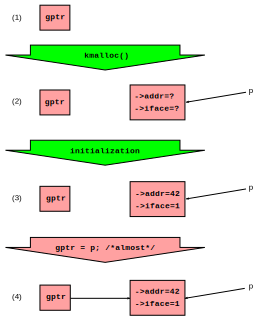
\includegraphics{defer/RCUListInsertClassic}}
\caption{Insertion With Concurrent Readers}
\label{fig:defer:Insertion With Concurrent Readers}
\end{figure}

To minimize implementability concerns, we focus on a minimal
data structure, which consists of a single global pointer that is either
\co{NULL} or references a single structure.
Minimal though it might be, this data structure is heavily used in
production~\cite{GeoffRomer2018C++DeferredReclamationP0561R4}.
A classic approach for insertion is shown in
Figure~\ref{fig:defer:Insertion With Concurrent Readers},
which shows four states with time advancing from top to bottom.
The first row shows the initial state, with \co{gptr} equal to \co{NULL}.
In the second row, we have allocated a structure which is uninitialized,
as indicated by the question marks.
In the third row, we have initialized the structure.
Finally, in the fourth and final row, we have updated \co{gptr} to
reference the newly allocated and initialized element.

We might hope that this assignment to \co{gptr} could use a simple
C-language assignment statement.
Unfortunately,
Section~\ref{sec:toolsoftrade:Shared-Variable Shenanigans}
dashes these hopes.
Therefore, the updater cannot use a simple C-language assignment, but
must instead use \co{smp_store_release()} as shown in the figure,
or, as will be seen, \co{rcu_assign_pointer()}.

Similarly, one might hope that readers could use a single C-language
assignment to fetch the value of \co{gptr}, and be guaranteed to either
get the old value of \co{NULL} or to get the newly installed pointer,
but either way see a valid result.
Unfortunately, Section~\ref{sec:toolsoftrade:Shared-Variable Shenanigans}
dashes these hopes as well.
To obtain this guarantee, readers must instead use \co{READ_ONCE()},
or, as will be seen, \co{rcu_dereference()}.
However, on most modern computer systems, each of these read-side primitives
can be implemented with a single load instruction, exactly the instruction
that would normally be used in single-threaded code.

Reviewing \cref{fig:defer:Insertion With Concurrent Readers}
from the viewpoint of readers, in the first three states all readers
see \co{gptr} having the value \co{NULL}.
Upon entering the fourth state, some readers might see \co{gptr} still
having the value \co{NULL} while others might see it referencing the
newly inserted element, but after some time, all readers will see this
new element.
At all times, all readers will see \co{gptr} as containing a valid pointer.
Therefore, it really is possible to add new data to linked data structures
while allowing concurrent readers to execute the same sequence of machine
instructions that is normally used in single-threaded code.
This no-cost approach to concurrent reading provides excellent performance
and scalability, and also is eminently suitable for real-time use.

\begin{figure}
\centering
\resizebox{3in}{!}{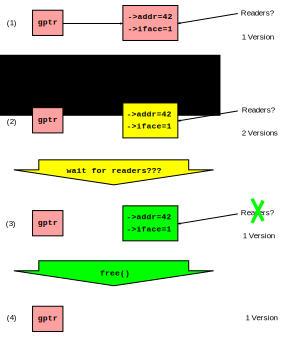
\includegraphics{defer/RCUListDeleteClassic}}
\caption{Deletion With Concurrent Readers}
\label{fig:defer:Deletion With Concurrent Readers}
\end{figure}

Insertion is of course quite useful, but sooner or later, it will also
be necessary to delete data.
As can be seen in
Figure~\ref{fig:defer:Deletion With Concurrent Readers},
the first step is easy.
Again taking the lessons from
Section~\ref{sec:toolsoftrade:Shared-Variable Shenanigans}
to heart, \co{smp_store_release()} is used to \co{NULL} the pointer,
thus moving from the first row to the second in the figure.
At this point, pre-existing readers see the old structure with
\co{->addr} of 42 and \co{->iface} of 1, but new readers will see
a \co{NULL} pointer, that is, concurrent readers can disagree on
the state, as indicated by the ``2 Versions'' in the figure.

\QuickQuizSeries{%
\QuickQuizB{
	Why does
	Figure~\ref{fig:defer:Deletion With Concurrent Readers}
	use \co{smp_store_release()} given that it is storing
	a \co{NULL} pointer?
	Wouldn't \co{WRITE_ONCE()} work just as well in this case,
	given that there is no structure initialization to order
	against the store of the \co{NULL} pointer?
}\QuickQuizAnswerB{
	Yes, it would.

	Because a \co{NULL} pointer is being assigned, there is nothing
	to order against, so there is no need for \co{smp_store_release()}.
	In contrast, when assigning a non-\co{NULL} pointer, it is
	necessary to use \co{smp_store_release()} in order to ensure
	that initialization of the pointed-to structure is carried
	out before assignment of the pointer.

	In short, \co{WRITE_ONCE()} would work, and would
	save a little bit of CPU time on some architectures.
	However, as we will see, software-engineering concerns
	will motivate use of a special \co{rcu_assign_pointer()}
	that is quite similar to \co{smp_store_release()}.
}\QuickQuizEndB
%
\QuickQuizE{
	Readers running concurrently each other and with the procedure
	outlined in
	Figure~\ref{fig:defer:Deletion With Concurrent Readers}
	can disagree on the value of \co{gptr}.
	Isn't that just a wee bit problematic???
}\QuickQuizAnswerE{
	Not necessarily.

	As hinted at in Sections~\ref{sec:cpu:Hardware Optimizations}
	and~\ref{sec:cpu:Hardware Free Lunch?},
	speed-of-light delays mean that a computer's data is always
	stale compared to whatever external reality that data is intended
	to model.

	Real-world algorithms therefore absolutely must tolerate
	inconsistancies between external reality and the in-computer
	data reflecting that reality.
	Many of those algorithms are also able to tolerate some degree
	of inconsistency within the in-computer data.
	Section~\ref{sec:datastruct:RCU-Protected Hash Table Discussion}
	discusses this point in more detail.

	Please note that this need to tolerate inconsistent and stale
	data is not limited to RCU\@.
	It also applies to reference counting, hazard pointers, sequence
	locks, and even to some locking use cases.
	For example, if you compute some quantity while holding a lock,
	but use that quantity after releasing that lock,
	you might well be using stale data.
	After all, the data that quantity is based on might change
	arbitrarily as soon as the lock is released.

	So yes, RCU readers can see stale and inconsistent data, but no,
	this is not necessarily problematic.
	And, when needed, there are RCU usage patterns that avoid both
	staleness and inconsistency~\cite{Arcangeli03}.
}\QuickQuizEndE
}

We get back to a single version simply by waiting for all the
pre-existing readers to complete, as shown in row~3.
At that point, all the pre-existing readers are done, and no later
reader has a path to the old data item, so there can no longer be
any readers referencing it.
It may therefore be safely freed, as shown on row~4.

Thus, given a way to wait for pre-existing readers to complete,
it is possible to both add data to and remove data from a linked
data structure, despite the readers executing the same sequence
of machine instructions that would be appropriate for single-threaded
execution.
So perhaps going all the way was not too far after all!

But how can we tell when all of the pre-existing readers have in
fact completed?
This question is the topic of the next section.

\subsubsection{Waiting for Readers}
\label{sec:defer:Waiting for Readers}

It is tempting to base reader waiting on reference counting, but
Figure~\ref{fig:count:Atomic Increment Scalability on x86}
in
Chapter~\ref{chp:Counting}
shows that concurrent reference counting results in extreme overhead,
as we already saw in
Section~\ref{sec:defer:Reference Counting}.
Hazard pointers profoundly reduce this overhead, but, as we saw in
Section~\ref{sec:defer:Hazard Pointers}, not to zero.
Nevertheless, many RCU implementations make very careful cache-local
use of counters.

A second approach observes that memory synchronization is expensive,
and therefore uses registers instead, namely each CPU's or thread's
program counter (PC), thus imposing no overhead on readers, at least
in the absence of concurrent updates.
The updater polls each relevant PC, and if that PC is not within read-side
code, then the corresponding CPU or thread is within a quiescent state,
in turn signaling the completion of any reader that might have access
to the newly removed data element.
Once all CPU's or thread's PCs have been observed to be outside of any
reader, the grace period has completed.
Please note that this approach poses some serious challenges, including
memory ordering, functions that are \emph{sometimes} invoked from readers,
and ever-exciting code-motion optimizations.
Nevertheless, this approach is said to be used in
production~\cite{MikeAsh2015Apple}.

A third approach is to simply wait for a fixed period of time that is
long enough to comfortably exceed the lifetime of any reasonable
reader~\cite{Jacobson93,AjuJohn95}.
This can work quite well in hard real-time systems~\cite{YuxinRen2018RTRCU},
but in less exotic
settings, Murphy says that it is critically important to be prepared
even for unreasonably long-lived readers.
To see this, consider the consequences of failing do so:
A data item will be freed while the unreasonable reader is still
referencing it, and that item might well be immediately reallocated,
possibly even as a data item of some other type.
The unreasonable reader and the unwitting reallocator would then
be attempting to use the same memory for two very different purposes.
The ensuing mess will at best be exceedingly difficult to debug.

A fourth approach is to wait forever, secure in the knowledge that
doing so will accommodate even the most unreasonable reader.
This approach is also called ``leaking memory'', and has a bad reputation
due to the fact that memory leaks often require untimely and
inconvenient reboots.
Nevertheless, this is a viable strategy when the update rate and the
uptime are both sharply bounded.
For example, this approach could work well in a high-availability
cluster where systems were periodically crashed in order to ensure
that cluster really remained highly available.\footnote{
	The program that forces the periodic crashing is sometimes
	known as a ``chaos monkey'':
	\url{https://netflix.github.io/chaosmonkey/}.
	However, it might also be a mistake to neglect chaos caused
	by systems running for too long.}
Leaking the memory is also a viable strategy in environments having
garbage collectors, in which case the garbage collector can be thought
of as plugging the leak~\cite{Kung80}.
However, if your environment lacks a garbage collector, read on!

A fifth approach avoids the period crashes in favor of periodically
``stopping the world'', as exemplified by the traditional stop-the-world
garbage collector.
This approach was also heavily used during the decades before
ubiquitous connectivity, when it was common practice to power systems
off at the end of each working day.
However, in today's always-connected always-on world, stopping the world
can gravely degrade response times, which has been one motivation for the
development of concurrent garbage collectors~\cite{DavidFBacon2003RTGC}.
Furthermore, although we need all pre-existing readers to complete, we do
not need them all to complete at the same time.

This observation leads to the sixth approach, which is stopping
one CPU or thread at a time.
This approach has the advantage of not degrading reader response times
at all, let alone gravely.
Furthermore, numerous applications already have states (termed
\emph{quiescent states}) that can be
reached only after all pre-existing readers are done.
In transaction-processing systems, the time between a pair of
successive transactions might be a quiescent state.
In reactive systems, the state between a pair of successive events
might be a quiescent state.
Within non-preemptive operating-systems kernels, a context switch can be
a quiescent state~\cite{McKenney98}.
Either way, once all CPUs and/or threads have passed through a quiescent
state, the system is said to have completed a \emph{grace period},
at which point all readers in existence at the start of that grace period
are guaranteed to have completed.
As a result, it is also guaranteed to be safe to free any removed data
items that were removed prior to the start of that grace period.\footnote{
	It is possible to do much more with RCU than simply defer
	reclamation of memory, but deferred reclamation is RCU's most
	common use case, and is therefore an excellent place to start.}

Within a non-preemptive operating-system kernel, for context switch to be
a valid quiescent state, readers must be prohibited from blocking while
referencing a given instance data structure obtained via the \co{gptr}
pointer shown in
Figures~\ref{fig:defer:Insertion With Concurrent Readers}
and~\ref{fig:defer:Deletion With Concurrent Readers}.
This no-blocking constraint is consistent with similar constraints
on pure spinlocks, where a CPU is forbidden from blocking while
holding a spinlock.
Without this constraint, all CPUs might be consumed by threads
spinning attempting to acquire a spinlock held by a blocked thread.
The spinning threads will not relinquish their CPUs until they acquire
the lock, but the thread holding the lock cannot possibly release it
until one of the spinning threads relinquishes a CPU\@.
This is a classic deadlock situation, and this deadlock is avoided
by forbidding blocking while holding a spinlock.

Again, this same constraint is imposed on reader threads dereferencing
\co{gptr}: such threads are not allowed to block until after
they are done using the pointed-to data item.
Returning to the second row of
Figure~\ref{fig:defer:Deletion With Concurrent Readers},
where the updater has just completed executing the \co{smp_store_release()},
imagine that CPU~0 executes a context switch.
Because readers are not permitted to block while traversing the linked
list, we are guaranteed that all prior readers that might have been running on
CPU~0 will have completed.
Extending this line of reasoning to the other CPUs, once each CPU has
been observed executing a context switch, we are guaranteed that all
prior readers have completed, and that there are no longer any reader
threads referencing the newly removed data element.
The updater can then safely free that data element, resulting in the
state shown at the bottom of
Figure~\ref{fig:defer:Deletion With Concurrent Readers}.

\begin{figure}
\centering
\resizebox{3in}{!}{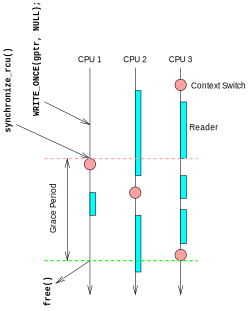
\includegraphics{defer/QSBRGracePeriod}}
\caption{QSBR: Waiting for Pre-Existing Readers}
\label{fig:defer:QSBR: Waiting for Pre-Existing Readers}
\end{figure}

This approach is termed \emph{quiescent state based reclamation}
(QSBR)~\cite{ThomasEHart2006a}.
A QSBR schematic is shown in
Figure~\ref{fig:defer:QSBR: Waiting for Pre-Existing Readers},
with time advancing from the top of the figure to the bottom.
CPU~1 does the \co{WRITE_ONCE()} that removes the current data
item (presumably having previously read the pointer value and
availed itself of appropriate synchronization), then waits
for readers.
This wait operation results in an immediate context switch, which is a
quiescent state (denoted by the pink circle), which in turn means that
all prior reads on CPU~1 have completed.
Next, CPU~2 does a context switch, so that all readers on CPUs~1 and~2
are now known to have completed.
Finally, CPU~3 does a context switch.
At this point, all readers throughout the entire system are known to
have completed, so the grace period ends, permitting CPU~1 to free
the old data item.

\QuickQuiz{
	In Figure~\ref{fig:defer:QSBR: Waiting for Pre-Existing Readers},
	the last of CPU~3's readers that could possibly have
	access to the old data item ended before the grace period
	even started!
	So why would anyone bother waiting until CPU~3's later context
	switch???
}\QuickQuizAnswer{
	Because that waiting is exactly what enables readers to use
	the same sequence of instructions that is appropriate for
	single-theaded situations.
	In other words, this additional ``redundant'' waiting enables
	excellent read-side performance, scalability, and real-time
	response.
}\QuickQuizEnd

\subsubsection{Toy Implementation}
\label{sec:defer:Toy Implementation}

Although production-quality QSBR implementations can be quite complex,
a toy non-preemptive Linux-kernel implementation is exceedingly simple:

\begin{VerbatimN}[samepage=true]
void synchronize_rcu(void)
{
	int cpu;

	for_each_online_cpu(cpu)
		sched_setaffinity(current->pid, cpumask_of(cpu));
}
\end{VerbatimN}

The \co{for_each_online_cpu()} primitive iterates over all CPUs, and
the \co{sched_setaffinity()} function causes the current thread to
execute on the specified CPU, which forces the destination CPU to execute
a context switch.
Therefore, once the \co{for_each_online_cpu()} has completed, each CPU
has executed a context switch, which in turn guarantees that
all pre-existing reader threads have completed.

\begin{listing}
\begin{fcvlabel}[ln:defer:Insertion and Deletion With Concurrent Readers]
\begin{VerbatimL}[commandchars=\\\[\]]
struct route *gptr;

int access_route(int (*f)(struct route *rp))
{
	int ret = -1;
	struct route *rp;

	rcu_read_lock();
	rp = rcu_dereference(gptr);
	if (rp)
		ret = f(rp);		\lnlbl[access_rp]
	rcu_read_unlock();
	return ret;
}

struct route *ins_route(struct route *rp)
{
	struct route *old_rp;

	spin_lock(&route_lock);
	old_rp = gptr;
	rcu_assign_pointer(gptr, rp);
	spin_unlock(&route_lock);
	return old_rp;
}

int del_route(void)
{
	struct route *old_rp;

	spin_lock(&route_lock);
	old_rp = gptr;
	RCU_INIT_POINTER(gptr, NULL);
	spin_unlock(&route_lock);
	synchronize_rcu();
	free(old_rp);
	return !!old_rp;
}
\end{VerbatimL}
\end{fcvlabel}
\caption{Insertion and Deletion With Concurrent Readers}
\label{lst:defer:Insertion and Deletion With Concurrent Readers}
\end{listing}

Please note that this approach is \emph{not} production quality.
Correct handling of a number of corner cases and the need for a number
of powerful optimizations mean that production-quality implementations
are quite complex.
In addition, RCU implementations for preemptible environments
require that readers actually do something, which in non-real-time
Linux-kernel environments can be as simple as defining
\co{rcu_read_lock()} and \co{rcu_read_unlock()} as \co{preempt_disable()}
and \co{preempt_enable()}, respectively.\footnote{
	Some toy RCU implementations that handle preempted
	read-side critical sections are shown in
	Appendix~\ref{chp:app:``Toy'' RCU Implementations}.}
However, this simple non-preemptible approach is conceptually complete,
and demonstrates that it really is possible to provide read-side
synchronization at zero cost, even in the face of concurrent updates.
In fact,
Listing~\ref{lst:defer:Insertion and Deletion With Concurrent Readers}
shows how reading (\co{access_route()}),
Figure~\ref{fig:defer:Insertion With Concurrent Readers}'s
insertion (\co{ins_route()}) and
Figure~\ref{fig:defer:Deletion With Concurrent Readers}'s
deletion (\co{del_route()}) can
be implemented.
(A slightly more capable routing table is shown in
Section~\ref{sec:defer:RCU for Pre-BSD Routing}.)

\QuickQuizSeries{%
\QuickQuizB{
	What is the point of \co{rcu_read_lock()} and \co{rcu_read_unlock()} in
	Listing~\ref{lst:defer:Insertion and Deletion With Concurrent Readers}?
	Why not just let the quiescent states speak for themselves?
}\QuickQuizAnswerB{
	Recall that readers are not permitted to pass through a quiescent
	state.
	For example, within the Linux kernel, RCU readers are not permitted
	to execute a context switch.
	Use of \co{rcu_read_lock()} and \co{rcu_read_unlock()} enables
	debug checks for improperly placed quiescent states, making it
	easy to find bugs that would otherwise be difficult to find,
	intermittent, and quite destructive.
}\QuickQuizEndB
%
\QuickQuizE{
	What is the point of \co{rcu_dereference()}, \co{rcu_assign_pointer()}
	and \co{RCU_INIT_POINTER()} in
	Listing~\ref{lst:defer:Insertion and Deletion With Concurrent Readers}?
	Why not just use \co{READ_ONCE()}, \co{smp_store_release()}, and
	\co{WRITE_ONCE()}, respectively?
}\QuickQuizAnswerE{
	The RCU-specific APIs do have similar semantics to the suggested
	replacements, but also enable static-analysis debugging checks
	that complain if an RCU-specific API is invoked on a non-RCU
	pointer and vice versa.
}\QuickQuizEndE
}

Referring back to
Listing~\ref{lst:defer:Insertion and Deletion With Concurrent Readers},
note that \co{route_lock} is used to synchronize between concurrent updaters
invoking \co{ins_route()} and \co{del_route()}.
However, this lock is not acquired by readers invoking \co{access_route()}:
Readers are instead protected by the QSBR techniques described in this section.

Note that \co{ins_route()} simply returns the old value of \co{gptr}, which
Figure~\ref{fig:defer:Insertion With Concurrent Readers} assumed would
always be \co{NULL}.
This means that it is the caller's responsibility to figure out what to
do with a non-\co{NULL} value, a task complicated by the fact that
readers might still be referencing it for an indeterminate period of time.
Callers might use one of the following approaches:

\begin{enumerate}
\item	Use \co{synchronize_rcu()} to safely free the pointed-to structure.
	Although this approach is correct from an RCU perspective, it
	arguably has software-engineering leaky-API problems.
\item	Trip an assertion if the returned pointer is non-\co{NULL}.
\item	Pass the returned pointer to a later invocation of
	\co{ins_route()} to restore the earlier value.
\end{enumerate}

In contrast, \co{del_route()} uses \co{synchronize_rcu()} and
\co{free()} to safely free the newly deleted data item.

\QuickQuiz{
	But what if the old structure needs to be freed, but the caller
	of \co{ins_route()} cannot block, perhaps due to performance
	considerations or perhaps because the caller is executing within
	an RCU read-side critical section?
}\QuickQuizAnswer{
	A \co{call_rcu()} function, which is described in
	Section~\ref{sec:defer:Wait For Pre-Existing RCU Readers},
	permits asynchronous grace-period waits.
}\QuickQuizEnd

This example shows one general approach to reading and updating
RCU-protected data structures, however, there is quite a variety
of use cases, several of which are covered in
Section~\ref{sec:defer:RCU Usage}.

In summary, it is in fact possible to create concurrent linked data
structures that can be traversed by readers executing the same sequence
of machine instructions that would be executed by single-threaded readers.
The next section summarizes RCU's high-level properties.

\subsubsection{RCU Properties}
\label{sec:defer:RCU Properties}

A key RCU property is that reads need not wait for updates.
This property enables RCU implementations to provide low-cost or even
no-cost readers, resulting in low overhead and excellent scalability.
This property also allows RCU readers and updaters to make useful
concurrent forward progress.
In contrast, conventional synchronization primitives must enforce strict
mutual exclusion using expensive instructions, thus increasing overhead
and degrading scalability, but also typically prohibiting readers and
updaters from making useful concurrent forward progress.

\QuickQuiz{
	Doesn't Section~\ref{sec:defer:Sequence Locks}'s seqlock
	also permit readers and updaters to make useful concurrent
	forward progress?
}\QuickQuizAnswer{
	Yes and no.
	Although seqlock readers can run concurrently with
	seqlock writers, whenever this happens, the \co{read_seqretry()}
	primitive will force the reader to retry.
	This means that any work done by a seqlock reader running concurrently
	with a seqlock updater will be discarded and the redone upon retry.
	So seqlock readers can \emph{run} concurrently with updaters,
	but they cannot actually get any work done in this case.

	In contrast, RCU readers can perform useful work even in presence
	of concurrent RCU updaters.

	However, both reference counters
	(Section~\ref{sec:defer:Reference Counting})
	and hazard pointers
	(Section~\ref{sec:defer:Hazard Pointers})
	really do permit useful concurrent forward progress for both
	updaters and readers, just at somewhat greater cost.
	Please see
	Section~\ref{sec:defer:Which to Choose?}
	for a comparison of these different solutions to the
	deferred-reclamation problem.
}\QuickQuizEnd

RCU delimits readers with \co{rcu_read_lock()} and \co{rcu_read_unlock()},
and ensures that each reader has a coherent view of each object
(see \cref{fig:defer:Deletion With Concurrent Readers}) by
maintaining multiple versions of objects and using update-side primitives
such as \co{synchronize_rcu()} to ensure that objects are not
freed until after the completion of all readers that might be using them.
RCU uses \co{rcu_assign_pointer()} and \co{rcu_dereference()} to provide
efficient and scalable mechanisms for publishing and reading new versions
of an object, respectively.
These mechanisms distribute the work among read and
update paths in such a way as to make read paths extremely fast, using
replication and weakening optimizations in a manner similar to
hazard pointers, but without the need for read-side retries.
In some cases, including \co{CONFIG_PREEMPT=n} Linux kernels,
RCU's read-side primitives have zero overhead.

But are these properties actually useful in practice?
This question is taken up by the next section.

\subsubsection{Practical Applicability}
\label{sec:defer:Practical Applicability}

\begin{figure}
\centering
\resizebox{3in}{!}{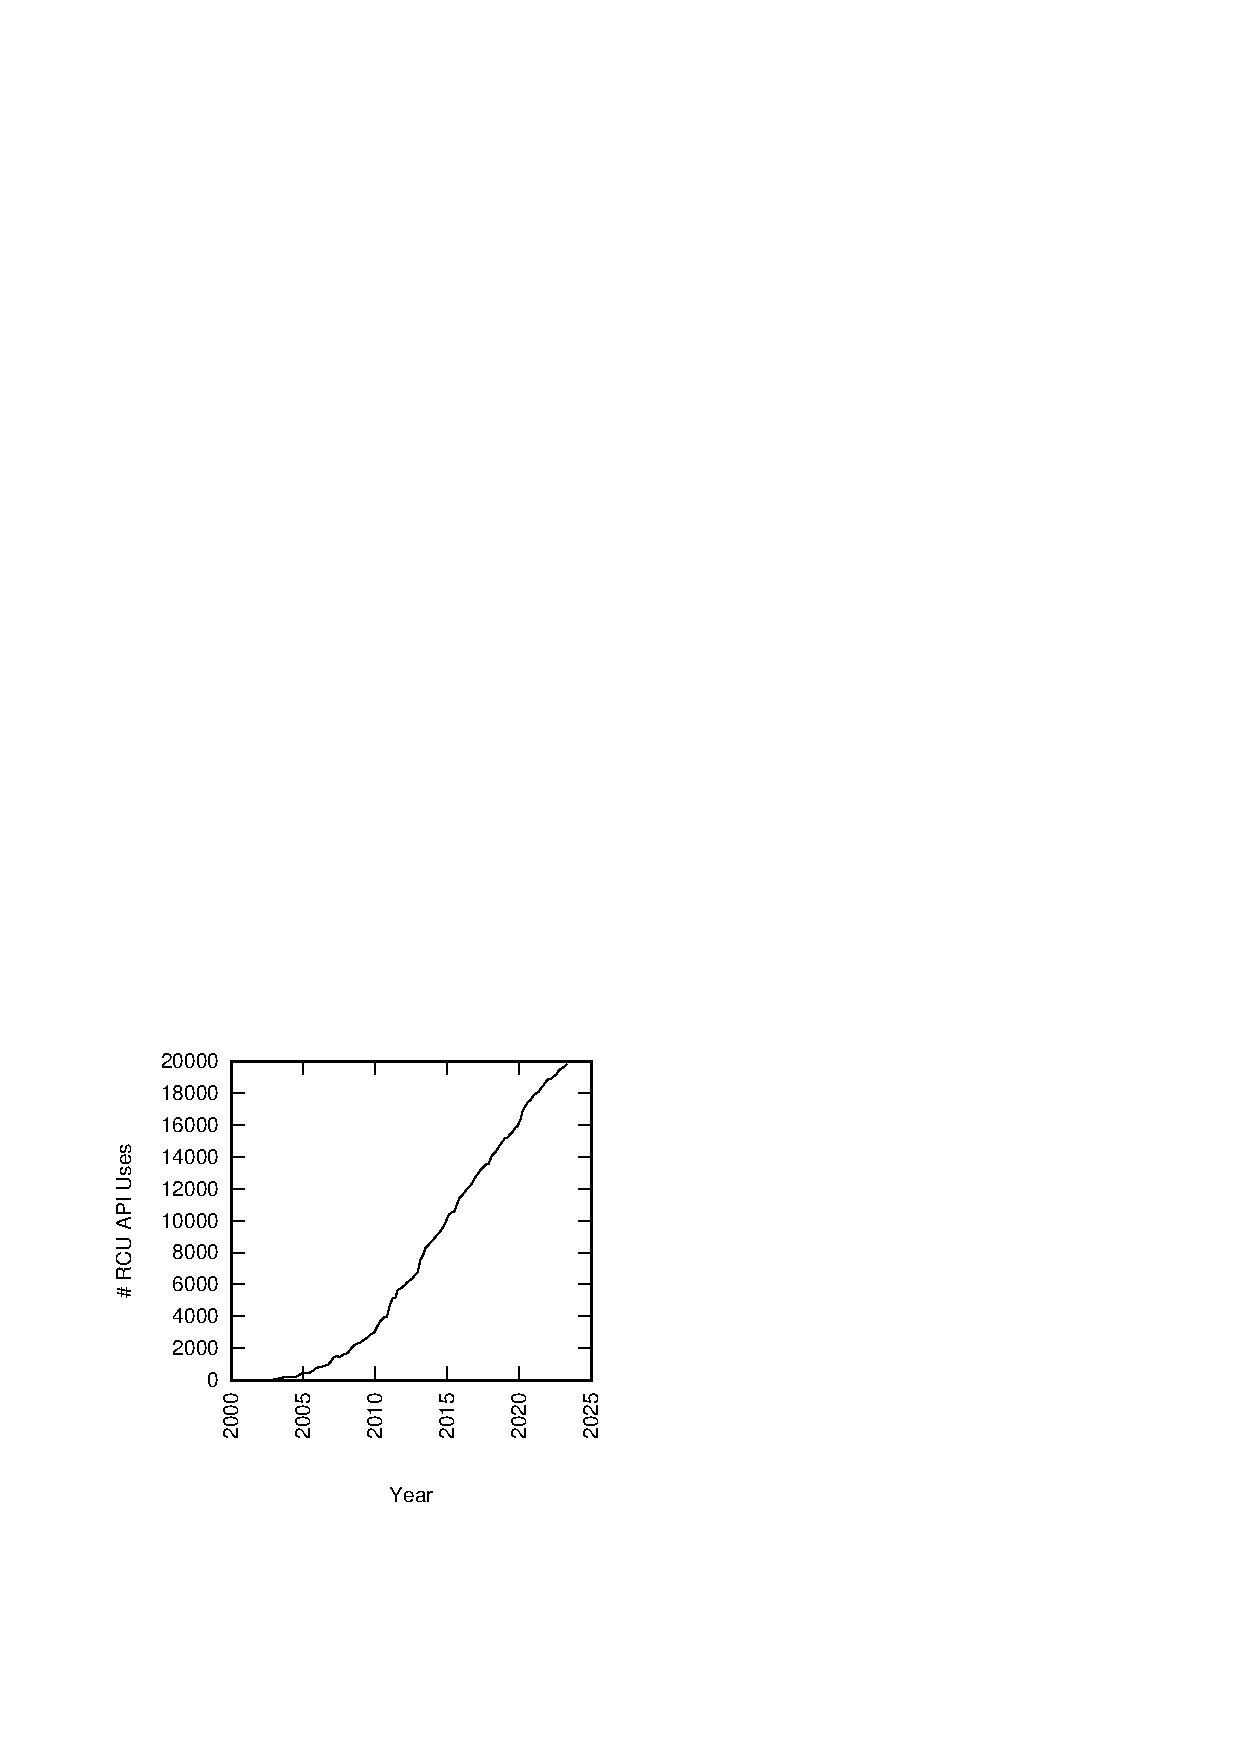
\includegraphics{defer/linux-RCU}}
\caption{RCU Usage in the Linux Kernel}
\label{fig:defer:RCU Usage in the Linux Kernel}
\end{figure}

RCU has been used in the Linux kernel since
October 2002~\cite{Torvalds2.5.43}.
Use of the RCU API has increased substantially since that time,
as can be seen in
Figure~\ref{fig:defer:RCU Usage in the Linux Kernel}.
In fact, code very similar to that in
Listing~\ref{lst:defer:Insertion and Deletion With Concurrent Readers}
is used in the Linux kernel.
RCU has enjoyed heavy use both prior to and since its acceptance
in the Linux kernel, as discussed in
\cref{sec:defer:RCU Related Work}.

It is therefore safe to say that RCU enjoys wide practical applicability.

The minimal example discussed in this section is a good introduction to RCU\@.
However, effective use of RCU often requires that you think differently
about your problem.
It is therefore useful to examine RCU's fundamentals, a task taken up
by the following section.

% defer/rcufundamental.tex
% mainfile: ../perfbook.tex
% SPDX-License-Identifier: CC-BY-SA-3.0

\subsection{RCU Fundamentals}
\label{sec:defer:RCU Fundamentals}
\OriginallyPublished{Section}{sec:defer:RCU Fundamentals}{RCU Fundamentals}{Linux Weekly News}{PaulEMcKenney2007WhatIsRCUFundamentally}

This section re-examines the ground covered in the previous section, but
independent of any particular example or use case.
People who prefer to live their lives very close to the actual code may
wish to skip the underlying fundamentals presented in this section.

RCU is made up of three fundamental mechanisms, the first being
used for insertion, the second being used for deletion, and the third
being used to allow readers to tolerate concurrent insertions and deletions.
Section~\ref{sec:defer:Publish-Subscribe Mechanism}
describes the publish-subscribe mechanism used for insertion,
Section~\ref{sec:defer:Wait For Pre-Existing RCU Readers}
describes how waiting for pre-existing RCU readers enabled deletion,
and
Section~\ref{sec:defer:Maintain Multiple Versions of Recently Updated Objects}
discusses how maintaining multiple versions of recently updated objects
permits concurrent insertions and deletions.
Finally,
Section~\ref{sec:defer:Summary of RCU Fundamentals}
summarizes RCU fundamentals.

\subsubsection{Publish-Subscribe Mechanism}
\label{sec:defer:Publish-Subscribe Mechanism}

Because RCU readers are not excluded by RCU updaters, an RCU-protected
data structure might change while a reader accesses it.
The accessed data item might be moved, removed, or replaced.
Because the data structure does not ``hold still'' for the reader,
each reader's access can be thought of as subscribing to the current
version of the RCU-protected data item.
For their part, updaters can be thought of as publishing new versions.

% @@@ Merge usage section into "Which to Choose?" and suggest choices.
% @@@ Should "RCU Exercises" move to "RCU Rescues"?

\begin{figure}[tbp]
\centering
\resizebox{3in}{!}{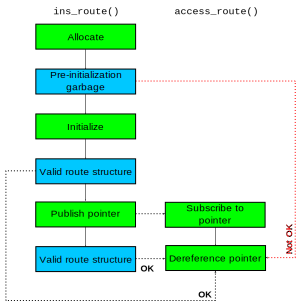
\includegraphics{defer/pubsub}}
\caption{Publication/Subscription Constraints}
\label{fig:defer:Publication/Subscription Constraints}
\end{figure}

Unfortunately, as laid out in
Section~\ref{sec:toolsoftrade:Shared-Variable Shenanigans}
and reiterated in
Section~\ref{sec:defer:Minimal Insertion and Deletion},
it is unwise to use plain accesses for these publication and subscription
operations.
It is instead necessary to inform both the compiler and the CPU
of the need for care, as can be seen from
Figure~\ref{fig:defer:Publication/Subscription Constraints},
which illustrates interactions between concurrent executions of
\co{ins_route()} (and its caller) and \co{read_gptr()} from
Listing~\ref{lst:defer:Insertion and Deletion With Concurrent Readers}.

The \co{ins_route()} column from
Figure~\ref{fig:defer:Publication/Subscription Constraints}
shows \co{ins_route()}'s caller allocating a new \co{route} structure,
which then contains pre-initialization garbage.
The caller then initializes the newly allocated structure, and then
invokes \co{ins_route()} to publish a pointer to the new \co{route}
structure.
Publication does not affect the contents of the structure, which
therefore remain valid after publication.

The \co{access_route()} column from this same figure shows
the pointer being subscribed to and dereferenced.
This dereference operation absolutely must see a valid \co{route}
structure rather than pre-initialization garbage because referencing
garbage could result in memory corruption, crashes, and hangs.
As noted earlier, avoiding such garbage means that the publish and
subscribe operations must inform both the compiler and the CPU of the
need to maintain the needed ordering.

Publication is carried out by \co{rcu_assign_pointer()}, which ensures that
\co{ins_route()}'s caller's initialization is ordered before the actual
publication operation's store of the pointer.
In addition, \co{rcu_assign_pointer()} must be atomic in the sense that 
concurrent readers see either the old value of the pointer or the new
value of the pointer, but not some mash-up of these two values.
These requirements are met by the C11 store-release operation, and in
fact in the Linux kernel, \co{rcu_assign_pointer()} is defined in terms
of \co{smp_store_release()}, which is similar to C11 store-release.

Note that if concurrent updates are required, some sort of synchronization
mechanism will be required to mediate among multiple concurrent
\co{rcu_assign_pointer()} calls on the same pointer.
In the Linux kernel, locking is the mechanism of choice, but pretty
much any synchronization mechanism may be used.
An example of a particularly lightweight synchronization mechanism is
Chapter~\ref{chp:Data Ownership}'s data ownership: If each pointer is
owned by a particular thread, then that thread may execute
\co{rcu_assign_pointer()} on that pointer with no additional
synchronization overhead.

\QuickQuiz{
	Wouldn't use of data ownership for RCU updaters mean that
	the updates could use exactly the same sequence of instructions
	as would the corresponding single-threaded code?
}\QuickQuizAnswer{
	Sometimes, for example, on TSO systems such as x86 or the IBM
	mainframe where a store-release operation emits a single store
	instruction.
	However, weakly ordered systems must also emit a memory barrier
	or perhaps a store-release instruction.
	In addition, removing data requires quite a bit of additional
	work because it is necessary to wait for pre-existing readers
	before freeing the removed data.
}\QuickQuizEnd

Subscription is carried out by \co{rcu_dereference()}, which orders
the subscription operation's load from the pointer is before the
dereference.
Similar to \co{rcu_assign_pointer()}, \co{rcu_dereference()} must be
atomic in the sense that the value loaded must be that from a single
store, for example, the compiler must not tear the load.\footnote{
	That is, the compiler must not break the load into multiple
	smaller loads, as described under ``load tearing'' in
	Section~\ref{sec:toolsoftrade:Shared-Variable Shenanigans}.}
Unfortunately, compiler support for \co{rcu_dereference()} is at best
a work in progress~\cite{PaulEMcKennneyConsumeP0190R4,PaulEMcKenney2017markconsumeP0462R1,JFBastien2018P0750R1consume}.
In the meantime, the Linux kernel relies on volatile loads, the details of
the various CPU architectures, coding
restrictions~\cite{PaulEMcKenney2014rcu-dereference},
and, on DEC Alpha~\cite{ALPHA2002}, a memory-barrier instruction.
However, on other architectures, \co{rcu_dereference()} typically
emits a single load instruction, just as would the equivalent single-threaded
code.
The coding restrictions are described in more detail in
Section~\ref{sec:memorder:Address- and Data-Dependency Difficulties},
however, the common case of field selection (\qtco{->}) works quite well.
Software that does not require the ultimate in read-side performance
can instead use C11 acquire loads, which provide the needed ordering and
more, albeit at a cost.
It is hoped that lighter-weight compiler support for \co{rcu_dereference()}
will appear in due course.

In short, use of \co{rcu_assign_pointer()} for publishing pointers and
use of \co{rcu_dereference()} for subscribing to them successfully avoids the
``Not OK'' garbage loads depicted in
Figure~\ref{fig:defer:Publication/Subscription Constraints}.
These two primitives can therefore be used to add new data to linked
structures without disrupting concurrent readers.

\QuickQuiz{
	But suppose that updaters are adding and removing multiple data
	items from a linked list while a reader is iterating over that
	same list.
	Specifically, suppose that a list initially contains elements
	A, B, and C, and that an updater removes element A and then
	adds a new element D at the end of the list.
	The reader might well see \{A, B, C, D\}, when that sequence of
	elements never actually ever existed!
	In what alternate universe would that qualify as ``not disrupting
	concurrent readers''???
}\QuickQuizAnswer{
	In the universe where an iterating reader is only required to
	traverse elements that were present throughout the full duration
	of the iteration.
	In the example, that would be elements B and C.
	Because elements A and D were each present for only part of the
	iteration, the reader is permitted to iterate over them, but not
	obliged to.
	Note that this supports the common case where the reader is simply
	looking up a single item, and does not know or care about the
	presence or absence of other items.

	If stronger consistency is required, then higher-cost
	synchronization mechanisms are required, for example, sequence
	locking or reader-writer locking.
	But if stronger consistency is \emph{not} required (and it very often
	is not), then why pay the higher cost?
}\QuickQuizEnd

Adding data to a linked structure without disrupting readers is a good thing,
as are the cases where this can be done with no added read-side cost compared
to single-threaded readers.
However, in most cases it is also necessary to remove data, and this is the
subject of the next section.

\subsubsection{Wait For Pre-Existing RCU Readers}
\label{sec:defer:Wait For Pre-Existing RCU Readers}

In its most basic form, RCU is a way of waiting for things to finish.
Of course, there are a great many other ways of waiting for things to
finish, including reference counts, reader-writer locks, events, and so on.
The great advantage of RCU is that it can wait for each of
(say) 20,000 different things without having to explicitly
track each and every one of them, and without having to worry about
the performance degradation, scalability limitations, complex deadlock
scenarios, and memory-leak hazards that are inherent in schemes
using explicit tracking.

In RCU's case, each of the things waited on is called an
\emph{RCU read-side critical section}.
As hinted at in
Section~\ref{sec:defer:Toy Implementation}, an RCU read-side critical
section starts with an \co{rcu_read_lock()} primitive, and ends with a
corresponding \co{rcu_read_unlock()} primitive.
RCU read-side critical sections can be nested, and may contain pretty
much any code, as long as that code does not contain a quiescent state,
for example, within the Linux kernel, it is illegal to sleep within
an RCU read-side critical section because a context switch is a quiescent
state.\footnote{
	However, a special form of RCU called SRCU~\cite{PaulEMcKenney2006c}
	does permit general sleeping in SRCU read-side critical sections.}
If you abide by these conventions, you can use RCU to wait for \emph{any}
pre-existing RCU read-side critical section to complete, and
\co{synchronize_rcu()} uses indirect means to do the actual
waiting~\cite{MathieuDesnoyers2012URCU,McKenney:2013:SDS:2483852.2483867}.

\begin{figure}[tbp]
\centering
\resizebox{3in}{!}{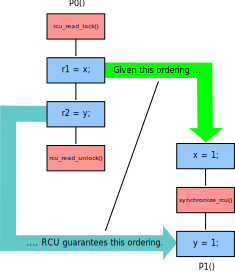
\includegraphics{defer/RCUGuaranteeFwd}}
\caption{RCU Reader and Later Grace Period}
\label{fig:defer:RCU Reader and Later Grace Period}
\end{figure}

The relationship between an RCU read-side critical section and a later
RCU grace period is an if-then relationship, as illustrated by
Figure~\ref{fig:defer:RCU Reader and Later Grace Period}.
If any portion of a given critical section precedes the beginning of
a given grace period, then RCU guarantees that all of that critical
section will precede the end of that grace period.
In the figure, \co{P0()}'s access to \co{x} precedes \co{P1()}'s access
to this same variable, and thus also precedes the grace period generated
by \co{P1()}'s call to \co{synchronize_rcu()}.
It is therefore guaranteed that \co{P0()}'s access to \co{y} will precede
\co{P1()}'s access.
In this case, if \co{r1}'s final value is 0, then \co{r2}'s final value
is guaranteed to also be 0.

\QuickQuiz{
	What other final values of \co{r1} and \co{r2} are possible in
	Figure~\ref{fig:defer:RCU Reader and Later Grace Period}?
}\QuickQuizAnswer{
	The \co{r1 == 0 && r2 == 0} possibility was called out in the text.
	Given that \co{r1 == 0} implies \co{r2 == 0}, we know that
	\co{r1 == 0 && r2 == 1} is forbidden.
	The following discussion will show that both
	\co{r1 == 1 && r2 == 1} and \co{r1 == 1 && r2 == 0} are possible.
}\QuickQuizEnd

\begin{figure}[tbp]
\centering
\resizebox{3in}{!}{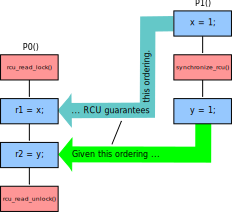
\includegraphics{defer/RCUGuaranteeRev}}
\caption{RCU Reader and Earlier Grace Period}
\label{fig:defer:RCU Reader and Earlier Grace Period}
\end{figure}

The relationship between an RCU read-side critical section and an earlier
RCU grace period is also an if-then relationship, as illustrated by
Figure~\ref{fig:defer:RCU Reader and Earlier Grace Period}.
If any portion of a given critical section follows the end of
a given grace period, then RCU guarantees that all of that critical
section will follow the beginning of that grace period.
In the figure, \co{P0()}'s access to \co{y} follows \co{P1()}'s access
to this same variable, and thus follows the grace period generated by
\co{P1()}'s call to \co{synchronize_rcu()}.
It is therefore guaranteed that \co{P0()}'s access to \co{x} will follow
\co{P1()}'s access.  In this case, if \co{r2}'s final value is 1, then
\co{r1}'s final value is guaranteed to also be 1.

\QuickQuiz{
	What would happen if the order of \co{P0()}'s two accesses was
	reversed in
	\cref{fig:defer:RCU Reader and Earlier Grace Period}?
}\QuickQuizAnswer{
	Absolutely nothing would change.
	The fact that \co{P0()}'s loads from \co{x} and \co{y} are
	in the same RCU read-side critical section suffices;
	their order is irrelevant.
}\QuickQuizEnd

\begin{figure}[tbp]
\centering
\resizebox{3in}{!}{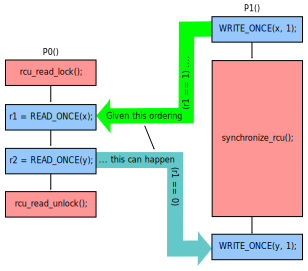
\includegraphics{defer/RCUGuaranteeMid}}
\caption{RCU Reader Within Grace Period}
\label{fig:defer:RCU Reader Within Grace Period}
\end{figure}

Finally, as shown in
Figure~\ref{fig:defer:RCU Reader Within Grace Period},
an RCU read-side critical section can be completely overlapped by
an RCU grace period.
In this case, \co{r1}'s final value is 1 and \co{r2}'s final value is 0.

However, it cannot be the case that \co{r1}'s final value is 0 and \co{r2}'s
final value is 1.
This would mean that an RCU read-side critical section had completely
overlapped a grace period, which is forbidden (or at the very least
constitutes a bug in RCU).
RCU's wait-for-readers guarantee therefore has two parts:
(1)~If any part of a given RCU read-side critical section precedes
the beginning of a given grace period, then the entirety of that
critical section precedes the end of that grace period.
(2)~If any part of a given RCU read-side critical section follows
the end of a given grace period, then the entirety of that
critical section follows the beginning of that grace period.
This definition is sufficient for almost all RCU-based algorithms, but
for those wanting more,
simple executable formal models of RCU are available
as part of Linux kernel v4.17 and later, as discussed in
Section~\ref{sec:formal:Axiomatic Approaches and RCU}.
In addition, RCU's ordering properties are examined in much
greater detail in Section~\ref{sec:memorder:RCU}.

\QuickQuiz{
	What would happen if \co{P0()}'s accesses in
	\crefrange{fig:defer:RCU Reader and Later Grace Period}{fig:defer:RCU Reader Within Grace Period}
	were stores?
}\QuickQuizAnswer{
	The exact same ordering rules would apply, that is,
	(1)~If any part of \co{P0()}'s RCU read-side critical section
	preceded the beginning of \co{P1()}'s grace period, all of
	\co{P0()}'s RCU read-side critical section would precede the
	end of \co{P1()}'s grace period, and
	(2)~If any part of \co{P0()}'s RCU read-side critical section
	followed the end of \co{P1()}'s grace period, all of \co{P0()}'s
	RCU read-side critical section would follow the beginning of
	\co{P1()}'s grace period.

	It might seem strange to have RCU read-side critical sections
	containing writes, but RCU is just fine with this.
	This capability is used frequently in the Linux kernel, for
	example, acquiring a lock on or reference to a data structure.
	Acquiring either a lock or a reference results in a write
	to memory, and it is OK to do these within an RCU read-side
	critical section.

	If having writes in RCU read-side critical sections still seems
	strange, please review
	\cref{sec:count:Applying Exact Limit Counters},
	which presented a use case for writes in reader-writer locking
	read-side critical sections.
}\QuickQuizEnd

Although RCU's wait-for-readers capability really is sometimes used to
order the assignment of values to variables as shown in
\crefrange{fig:defer:RCU Reader and Later Grace Period}
{fig:defer:RCU Reader Within Grace Period},
it is more frequently used to safely free data elements removed from
a linked structure, as was done in
Section~\ref{sec:defer:Introduction to RCU}.
The general process is illustrated by the following pseudocode:

\begin{enumerate}
\item	Make a change, for example, remove an element from a linked list.
\item	Wait for all pre-existing RCU read-side critical sections to
	completely finish (for example, by using
	\co{synchronize_rcu()}).
\item	Clean up, for example, free the element that was replaced above.
\end{enumerate}

\begin{figure}[tbp]
\centering
\resizebox{2.5in}{!}{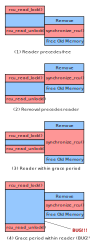
\includegraphics{defer/RCUGPorderingSummary}}
\caption{Summary of RCU Grace-Period Ordering Guarantees}
\label{fig:defer:Summary of RCU Grace-Period Ordering Guarantees}
\end{figure}

This more abstract procedure requires a more abstract diagram than
\crefrange{fig:defer:RCU Reader and Later Grace Period}
{fig:defer:RCU Reader Within Grace Period},
which are specific to a particular litmus test.
After all, and RCU implementation must work correctly regardless of
the form of the RCU updates and the RCU read-side critical sections.
Figure~\ref{fig:defer:Summary of RCU Grace-Period Ordering Guarantees}
fills this need, showing the four possible scenarios, with time
advancing from top to bottom within each scenario.
Within each scenario, an RCU reader is represented by the left-hand
stack of boxes and RCU updater by the right-hand stack.

In the first scenario, the reader starts execution before the
updater starts the removal, so it is possible that this reader
has a reference to the removed data element.
Therefore, the updater must not free this element until after the
reader completes.
In the second scenario, the reader does not start execution until
after the removal has completed.
The reader cannot possibly obtain a reference to the already-removed
data element, so this element may be freed before the reader completes.
The third scenario is like the second, but illustrates that when the
reader cannot possibly obtain a reference to element, it is still
permissible to defer the freeing of that element until after the
reader completes.
In the fourth and final scenario, the reader starts execution before
the updater starts removing the data element, but this element
is (incorrectly) freed before the reader completed.
A correct RCU implementation will not allow this fourth scenario to
occur.
This diagram thus illustrates RCU's wait-for-readers functionality:
Given a grace period, each reader ends before the end of that grace
period, starts after the beginning of that grace period, or both, in
which case it is wholly contained within that grace period.

Because RCU readers can make forward progress while updates
are in progress, different readers might disagree about the state
of the data structure, a topic taken up by the next section.

\subsubsection{Maintain Multiple Versions of Recently Updated Objects}
\label{sec:defer:Maintain Multiple Versions of Recently Updated Objects}

This section discusses how RCU accommodates synchronization-free readers
by maintaining multiple versions of data.
This discussion builds on the introduction of multiple versions by
Figure~\ref{fig:defer:Deletion With Concurrent Readers}
in
Section~\ref{sec:defer:Minimal Insertion and Deletion},
in which readers running concurrently with \co{del_route()}
(see Listing~\ref{lst:defer:Insertion and Deletion With Concurrent Readers})
might see the old \co{route} structure or an empty list, but either
way get a valid result.
Of course, a closer look at
Figure~\ref{fig:defer:Insertion With Concurrent Readers}
shows that calls to \co{ins_route()} can also result in concurrent
readers seeing different versions: Either the initial empty list
or the newly inserted \co{route} structure.
Note that both reference counting
(Section~\ref{sec:defer:Reference Counting})
and hazard pointers
(Section~\ref{sec:defer:Hazard Pointers})
can also cause concurrent readers to see different versions, but
RCU's lightweight readers make this more likely.

\begin{figure}[tbp]
\centering
\resizebox{3in}{!}{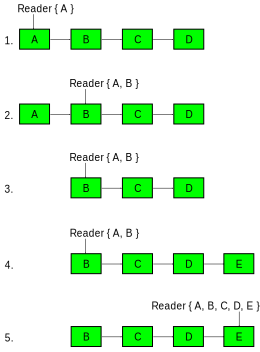
\includegraphics{defer/multver}}
\caption{Multiple RCU Data-Structure Versions}
\label{fig:defer:Multiple RCU Data-Structure Versions}
\end{figure}

However, maintaining multiple versions can be even more surprising.
For example, consider
Figure~\ref{fig:defer:Multiple RCU Data-Structure Versions},
in which a reader is traversing a linked list that is concurrently
updated.\footnote{
	RCU linked-list APIs may be found in
	Section~\ref{sec:defer:RCU Linux-Kernel API}.}
In the first row of the figure, the reader is referencing data item~A,
and in the second row, it advances to~B, having thus far seen A followed by~B.
In the third row, an updater removes element~A and in the fourth row
an updater adds element~E to the end of the list.
In the fifth and final row, the reader completes its traversal, having
seeing elements A through E.

Except that there was no time at which such a list existed.
This situation might be even more surprising than that shown in
Figure~\ref{fig:defer:Deletion With Concurrent Readers},
in which different concurrent readers see different versions.
In contrast, in
Figure~\ref{fig:defer:Multiple RCU Data-Structure Versions}
the reader sees a version that never actually existed!

One way to resolve this strange situation is via weaker semanitics.
A reader traversal must encounter any data item that was present
during the full traversal (B, C, and~D), and might or might not
encounter data items that were present for only part of the
traversal (A and~E).
Therefore, in this particular case, it is perfectly legitimate for
the reader traveral to encounter all five elements.
If this outcome is problematic, another way to resolve this situation is
through use of stronger synchronization mechanisms, such as reader-writer
locking or clever use of timestamps or versioning.
Of course, stronger mechanisms will be more expensive, but then again
the engineering life is all about choices and tradeoffs.

Strange though this situation might seem, it is entirely consistent with
the real world.
As we saw in
Section~\ref{sec:cpu:Overheads},
the finite speed of light cannot be ignored within a computer system,
and it most certainly cannot be ignored outside of this system.
This in turn means that any data within the system representing state
in the real world outside of the system is always and forever outdated,
and thus inconsistent with the real world.
As a result, algorithms operating on real-world data must account for
inconsistent data.
In many cases, these algorithms are also perfectly capable of dealing
with inconsistencies within the system.

The pre-BSD packet routing example laid out in
Section~\ref{sec:defer:Running Example}
is a case in point.
The contents of a routing list is set by routing protocols, and these
protocols feature significant delays (seconds or even minutes) to avoid
routing instabilities.
Therefore, once a routing update reaches a given system,
it might well have been sending packets the wrong way for quite some time.
Sending a few more packets the wrong way for the few microseconds during
which the update is in flight is clearly not a problem because the same
higher-level protocol actions that deal with delayed routing updates
will also deal with internal inconsistencies.

Nor is Internet routing the only situation tolerating inconsistencies.
To repeat, any algorithm in which data within a system tracks
outside-of-system state must tolerate inconsistencies, which includes
security policies (often set by committees of humans), storage configuration,
and WiFi access points, to say nothing of removable hardware such as
microphones, headsets, cameras, mice, printers, and much else besides.
Furthermore, the large number of Linux-kernel RCU API uses shown in
Figure~\ref{fig:defer:RCU Usage in the Linux Kernel},
combined with the Linux kernel's heavy use of reference counting
and with increasing use of hazard pointers in other projects, demonstrates
that tolerance for such inconsistencies is more common than one might
imagine.
This is especially the case given that single-item lookups are much more
common than traversals:  After all, (1)~concurrent updates are less likely
to affect a single-item lookup than they are a full traversal, and
(2)~an isolated single-item lookup cannot detect such inconsistencies.

From a more theoretical viewpoint, there are even some special cases where
RCU readers can be considered to be fully ordered with updaters, despite
the fact that these readers might be executing the exact same sequence of
machine instructions that would be executed by a single-threaded program.
For example, referring back to
Listing~\ref{lst:defer:Insertion and Deletion With Concurrent Readers}
on page~\pageref{lst:defer:Insertion and Deletion With Concurrent Readers},
suppose that each reader thread invokes \co{access_route()} exactly
once during its lifetime, and that there is no other communication among
reader and updater threads.
\begin{fcvref}[ln:defer:Insertion and Deletion With Concurrent Readers]
Then each invocation of \co{access_route()} can be ordered after the
\co{ins_route()} invocation that produced the \co{route} structure
accessed by \clnref{access_rp} of the listing in \co{access_route()}
and ordered before any subsequent
\co{ins_route()} or \co{del_route()} invocation.
\end{fcvref}

In summary, maintaining multiple versions is exactly what enables the
extremely low overheads of RCU readers, and as noted earlier, many
algorithms are unfazed by multiple versions.
However, there are algorithms that absolutely cannot handle multiple versions.
There are techniques for adapting such algorithms to
RCU~\cite{PaulEdwardMcKenneyPhD},
but these are beyond the scope of this section.

\paragraph{Exercises}
\label{sec:defer:Exercises}

These examples assumed that a mutex was held across the entire
update operation, which would mean that there could be at most two
versions of the list active at a given time.

\QuickQuizSeries{%
\QuickQuizB{
	How would you modify the deletion example to permit more than two
	versions of the list to be active?
}\QuickQuizAnswerB{
	One way of accomplishing this is as shown in
	Listing~\ref{lst:defer:Concurrent RCU Deletion}.

\begin{listing}[htbp]
\begin{VerbatimL}
spin_lock(&mylock);
p = search(head, key);
if (p == NULL)
	spin_unlock(&mylock);
else {
	list_del_rcu(&p->list);
	spin_unlock(&mylock);
	synchronize_rcu();
	kfree(p);
}
\end{VerbatimL}
\caption{Concurrent RCU Deletion}
\label{lst:defer:Concurrent RCU Deletion}
\end{listing}

	Note that this means that multiple concurrent deletions might be
	waiting in \co{synchronize_rcu()}.
}\QuickQuizEndB
%
\QuickQuizE{
	How many RCU versions of a given list can be
	active at any given time?
}\QuickQuizAnswerE{
	That depends on the synchronization design.
	If a semaphore protecting the update is held across the grace period,
	then there can be at most two versions, the old and the new.

	However, suppose that only the search, the update, and the
	\co{list_replace_rcu()} were protected by a lock, so that
	the \co{synchronize_rcu()} was outside of that lock, similar
	to the code shown in
	Listing~\ref{lst:defer:Concurrent RCU Deletion}.
	Suppose further that a large number of threads undertook an
	RCU replacement at about the same time, and that readers
	are also constantly traversing the data structure.

	Then the following sequence of events could occur, starting from
	the end state of
	Figure~\ref{fig:defer:Multiple RCU Data-Structure Versions}:

	\begin{enumerate}
	\item	Thread~A traverses the list, obtaining a reference to
		Element~C.
	\item	Thread~B replaces Element~C with a new
		Element~F, then waits for its \co{synchronize_rcu()}
		call to return.
	\item	Thread~C traverses the list, obtaining a reference to
		Element~F.
	\item	Thread~D replaces Element~F with a new
		Element~G, then waits for its \co{synchronize_rcu()}
		call to return.
	\item	Thread~E traverses the list, obtaining a reference to
		Element~G.
	\item	Thread~F replaces Element~G with a new
		Element~H, then waits for its \co{synchronize_rcu()}
		call to return.
	\item	Thread~G traverses the list, obtaining a reference to
		Element~H.
	\item	And the previous two steps repeat quickly with additional
		new elements, so that all of them happen before any of
		the \co{synchronize_rcu()} calls return.
	\end{enumerate}

	Thus, there can be an arbitrary number of versions active,
	limited only by memory and by how many updates could be completed
	within a grace period.
	But please note that data structures that are updated so frequently
	are not likely to be good candidates for RCU.
	Nevertheless, RCU can handle high update rates when necessary.
}\QuickQuizEndE
}

\subsubsection{Summary of RCU Fundamentals}
\label{sec:defer:Summary of RCU Fundamentals}

This section has described the three fundamental components of RCU-based
algorithms:

\begin{enumerate}
\item	a publish-subscribe mechanism for adding new data,

\item	a way of waiting for pre-existing RCU readers to finish
	(see Section~\ref{sec:memorder:RCU} for more detail),
	and

\item	a discipline of maintaining multiple versions to permit
	change without harming or unduly delaying concurrent RCU readers.
\end{enumerate}

\QuickQuiz{
	How can RCU updaters possibly delay RCU readers, given that
	neither \co{rcu_read_lock()} nor \co{rcu_read_unlock()}
	spin or block?
}\QuickQuizAnswer{
	The modifications undertaken by a given RCU updater will cause the
	corresponding CPU to invalidate cache lines containing the data,
	forcing the CPUs running concurrent RCU readers to incur expensive
	cache misses.
	(Can you design an algorithm that changes a data structure
	\emph{without}
	inflicting expensive cache misses on concurrent readers?
	On subsequent readers?)
}\QuickQuizEnd

These three RCU components allow data to be updated in face of concurrent
readers that might be executing the same sequence of machine instructions
that would be used by a reader in a single-threaded implementation.
These RCU components can be combined in different ways to implement a
surprising variety of different types of RCU-based algorithms.
However, it is usually better to work at higher levels of abstraction.
To this end, the next section describes the Linux-kernel API, which
includes simple data structures such as lists.

% defer/rcuusage.tex

\subsection{RCU Usage}
\label{sec:defer:RCU Usage}
\OriginallyPublished{Section}{sec:defer:RCU Usage}{RCU Usage}{Linux Weekly News}{PaulEMcKenney2008WhatIsRCUUsage}

\begin{table}[tb]
\centering
\scriptsize
\begin{tabular}{l|l}
Mechanism RCU Replaces & Section \\
\hline
\hline
Reader-writer locking &
	Section~\ref{sec:defer:RCU is a Reader-Writer Lock Replacement} \\
Restricted reference-counting mechanism &
	Section~\ref{sec:defer:RCU is a Restricted Reference-Counting Mechanism} \\
Bulk reference-counting mechanism &
	Section~\ref{sec:defer:RCU is a Bulk Reference-Counting Mechanism} \\
Poor man's garbage collector &
	Section~\ref{sec:defer:RCU is a Poor Man's Garbage Collector} \\
Existence Guarantees &
	Section~\ref{sec:defer:RCU is a Way of Providing Existence Guarantees} \\
Type-Safe Memory &
	Section~\ref{sec:defer:RCU is a Way of Providing Type-Safe Memory} \\
Wait for things to finish &
	Section~\ref{sec:defer:RCU is a Way of Waiting for Things to Finish} \\
\end{tabular}
\caption{RCU Usage}
\label{tab:defer:RCU Usage}
\end{table}

This section answers the question ``What is RCU?'' from the viewpoint
of the uses to which RCU can be put.
Because RCU is most frequently used to replace some existing mechanism,
we look at it primarily in terms of its relationship to such mechanisms,
as listed in Table~\ref{tab:defer:RCU Usage}.
Following the sections listed in this table,
Section~\ref{sec:defer:RCU Usage Summary} provides a summary.

\subsubsection{RCU for Pre-BSD Routing}
\label{sec:defer:RCU for Pre-BSD Routing}

\begin{figure}[tbp]
{ \scriptsize
\begin{verbbox}
 1 struct route_entry {
 2   struct rcu_head rh;
 3   struct cds_list_head re_next;
 4   unsigned long addr;
 5   unsigned long iface;
 6   int re_freed;
 7 };
 8 CDS_LIST_HEAD(route_list);
 9 DEFINE_SPINLOCK(routelock);
10
11 unsigned long route_lookup(unsigned long addr)
12 {
13   struct route_entry *rep;
14   unsigned long ret;
15
16   rcu_read_lock();
17   cds_list_for_each_entry_rcu(rep, &route_list,
18                               re_next) {
19     if (rep->addr == addr) {
20       ret = rep->iface;
21       if (READ_ONCE(rep->re_freed))
22         abort();
23       rcu_read_unlock();
24       return ret;
25     }
26   }
27   rcu_read_unlock();
28   return ULONG_MAX;
29 }
\end{verbbox}
}
\centering
\theverbbox
\caption{RCU Pre-BSD Routing Table Lookup}
\label{fig:defer:RCU Pre-BSD Routing Table Lookup}
\end{figure}

\begin{figure}[tbp]
{ \scriptsize
\begin{verbbox}
 1 int route_add(unsigned long addr,
 2               unsigned long interface)
 3 {
 4   struct route_entry *rep;
 5
 6   rep = malloc(sizeof(*rep));
 7   if (!rep)
 8     return -ENOMEM;
 9   rep->addr = addr;
10   rep->iface = interface;
11   rep->re_freed = 0;
12   spin_lock(&routelock);
13   cds_list_add_rcu(&rep->re_next, &route_list);
14   spin_unlock(&routelock);
15   return 0;
16 }
17
18 static void route_cb(struct rcu_head *rhp)
19 {
20   struct route_entry *rep;
21
22   rep = container_of(rhp, struct route_entry, rh);
23   WRITE_ONCE(rep->re_freed, 1);
24   free(rep);
25 }
26
27 int route_del(unsigned long addr)
28 {
29   struct route_entry *rep;
30
31   spin_lock(&routelock);
32   cds_list_for_each_entry(rep, &route_list,
33                           re_next) {
34     if (rep->addr == addr) {
35       cds_list_del_rcu(&rep->re_next);
36       spin_unlock(&routelock);
37       call_rcu(&rep->rh, route_cb);
38       return 0;
39     }
40   }
41   spin_unlock(&routelock);
42   return -ENOENT;
43 }
\end{verbbox}
}
\centering
\theverbbox
\caption{RCU Pre-BSD Routing Table Add/Delete}
\label{fig:defer:RCU Pre-BSD Routing Table Add/Delete}
\end{figure}

Figures~\ref{fig:defer:RCU Pre-BSD Routing Table Lookup}
and~\ref{fig:defer:RCU Pre-BSD Routing Table Add/Delete}
show code for an RCU-protected Pre-BSD routing table
(\path{route_rcu.c}).
The former shows data structures and \co{route_lookup()},
and the latter shows \co{route_add()} and \co{route_del()}.

In Figure~\ref{fig:defer:RCU Pre-BSD Routing Table Lookup},
line~2 adds the \co{->rh} field used by RCU reclamation,
line~6 adds the \co{->re_freed} use-after-free-check field,
lines~16, 17, 23, and~27 add RCU read-side protection,
and lines~21 and~22 add the use-after-free check.
In Figure~\ref{fig:defer:RCU Pre-BSD Routing Table Add/Delete},
lines~12, 14, 31, 36, and~41 add update-side locking,
lines~13 and~35 add RCU update-side protection,
line~37 causes \co{route_cb()} to be invoked after a grace period elapses,
and lines~18-25 define \co{route_cb()}.
This is minimal added code for a working concurrent implementation.

\begin{figure}[tb]
\centering
\resizebox{2.5in}{!}{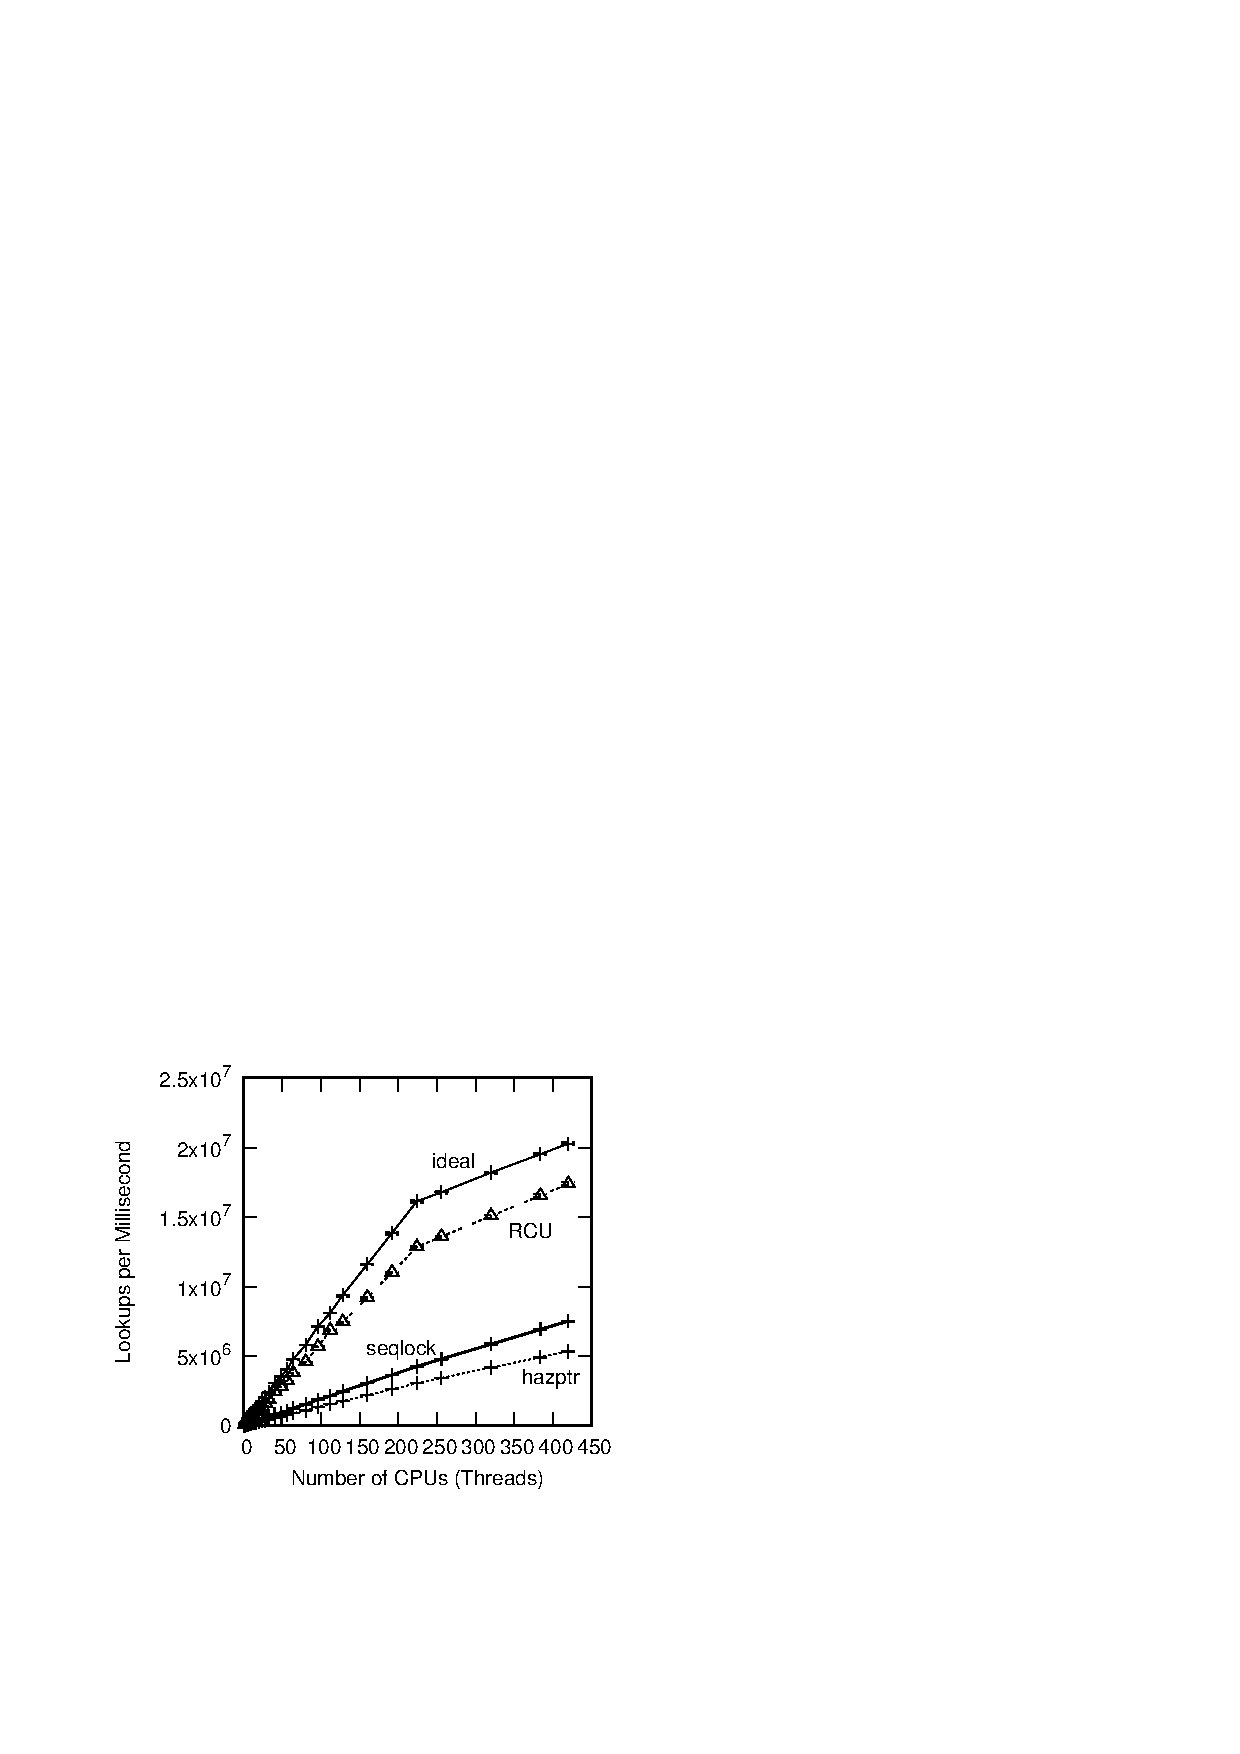
\includegraphics{CodeSamples/defer/perf-rcu}}
\caption{Pre-BSD Routing Table Protected by RCU}
\label{fig:defer:Pre-BSD Routing Table Protected by RCU}
\end{figure}

Figure~\ref{fig:defer:Pre-BSD Routing Table Protected by RCU}
shows the performance on the read-only workload.
RCU scales quite well, and offers nearly ideal performance.
However, this data was generated using the \co{RCU_SIGNAL}
flavor of userspace
RCU~\cite{MathieuDesnoyers2009URCU,PaulMcKenney2013LWNURCU},
for which \co{rcu_read_lock()} and \co{rcu_read_unlock()}
generate a small amount of code.
What happens for the QSBR flavor of RCU, which generates no code at all
for \co{rcu_read_lock()} and \co{rcu_read_unlock()}?
(See Section~\ref{sec:defer:Introduction to RCU},
and especially
Figure~\ref{fig:defer:RCU QSBR: Waiting for Pre-Existing Readers},
for a discussion of RCU QSBR.)

The answer to this shown in
Figure~\ref{fig:defer:Pre-BSD Routing Table Protected by RCU QSBR},
which shows the RCU QSBR results as the trace between the RCU and
the ideal traces.
RCU QSBR's performance and scalability is very nearly that of an
ideal synchronization-free workload, as desired.

\QuickQuiz{}
	Why doesn't RCU QSBR give \emph{exactly} ideal results?
\QuickQuizAnswer{
	The \co{rcu_dereference()} primitive does constrain the
	compiler's optimizations somewhat, which can result in
	slightly slower code.
	This effect would normally be insignificant, but
	each search is taking on average about 13~nanoseconds,
	which is short enough for small differences in code
	generation to make their presence felt.
	The difference ranges from about 1.5\% to about 11.1\%, which is
	quite small when you consider that the RCU QSBR code can handle
	concurrent updates and the ``ideal'' code cannot.

	It is hoped that C11 \co{memory_order_consume}
	loads~\cite{RichardSmith2015N4527}
	might someday allow \co{rcu_dereference()} provide the
	needed protection at lower cost.
} \QuickQuizEnd

\QuickQuiz{}
	Given RCU QSBR's read-side performance, why bother with any
	other flavor of userspace RCU?
\QuickQuizAnswer{
	Because RCU QSBR places constraints on the overall application
	that might not be tolerable,
	for example, requiring that each and every thread in the
	application regularly pass through a quiescent state.
	Among other things, this means that RCU QSBR is not helpful
	to library writers, who might be better served by other
	flavors of userspace RCU~\cite{PaulMcKenney2013LWNURCU}.
} \QuickQuizEnd

\begin{figure}[tb]
\centering
\resizebox{2.5in}{!}{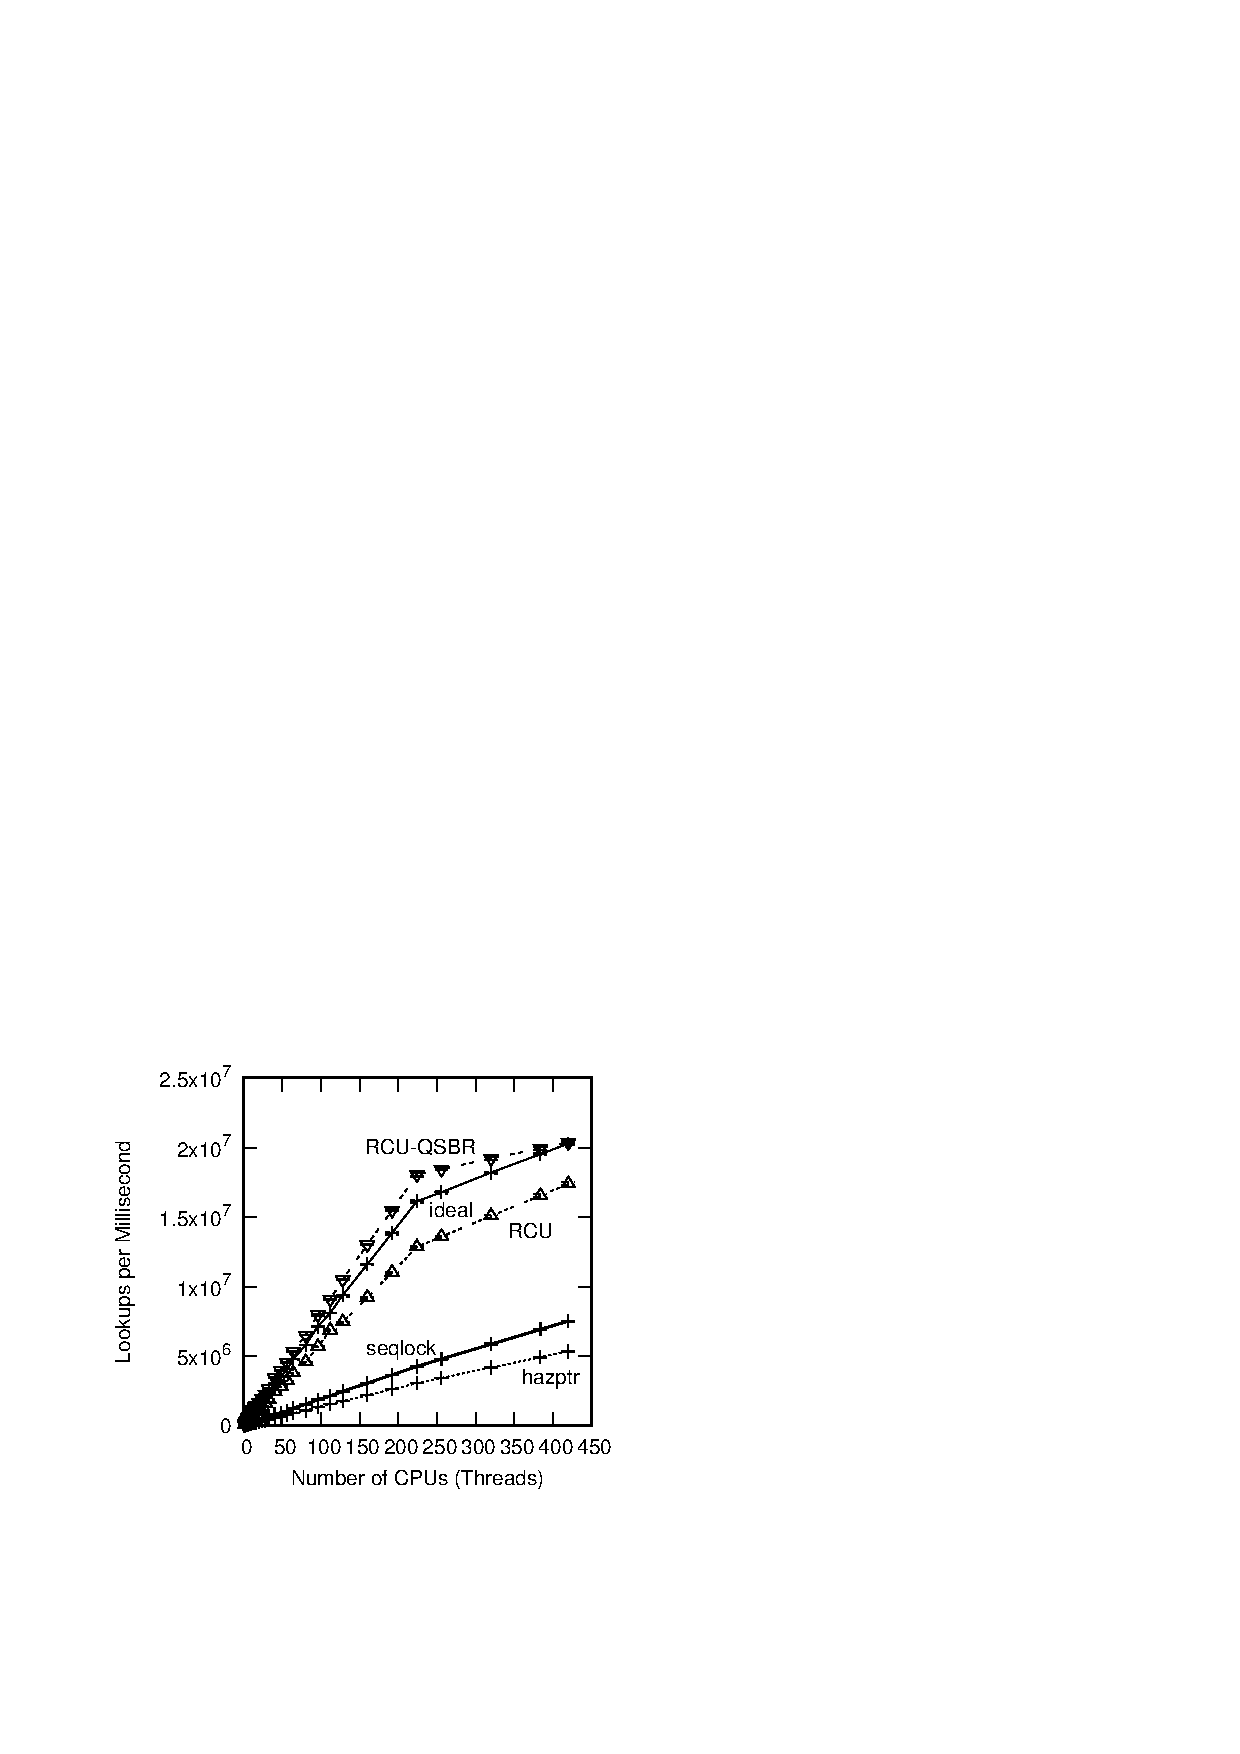
\includegraphics{CodeSamples/defer/perf-rcu-qsbr}}
\caption{Pre-BSD Routing Table Protected by RCU QSBR}
\label{fig:defer:Pre-BSD Routing Table Protected by RCU QSBR}
\end{figure}

\subsubsection{RCU is a Reader-Writer Lock Replacement}
\label{sec:defer:RCU is a Reader-Writer Lock Replacement}

Perhaps the most common use of RCU within the Linux kernel is as
a replacement for reader-writer locking in read-intensive situations.
Nevertheless, this use of RCU was not immediately apparent to me
at the outset, in fact, I chose to implement a lightweight reader-writer
lock~\cite{WilsonCHsieh92a}\footnote{
	Similar to \co{brlock} in the 2.4 Linux kernel and to
	\co{lglock} in more recent Linux kernels.}
before implementing a general-purpose RCU implementation
back in the early 1990s.
Each and every one of the uses I envisioned for the lightweight reader-writer
lock was instead implemented using RCU.
In fact, it was more than
three years before the lightweight reader-writer lock saw its first use.
Boy, did I feel foolish!

The key similarity between RCU and reader-writer locking is that
both have read-side critical sections that can execute in parallel.
In fact, in some cases, it is possible to mechanically substitute RCU API
members for the corresponding reader-writer lock API members.
But first, why bother?

Advantages of RCU include performance,
deadlock immunity, and realtime latency.
There are, of course, limitations to RCU, including the fact that
readers and updaters run concurrently, that low-priority RCU readers
can block high-priority threads waiting for a grace period to elapse,
and that grace-period latencies can extend for many milliseconds.
These advantages and limitations are discussed in the following sections.

\paragraph{Performance}

\begin{figure}[tb]
\centering
\resizebox{2.5in}{!}{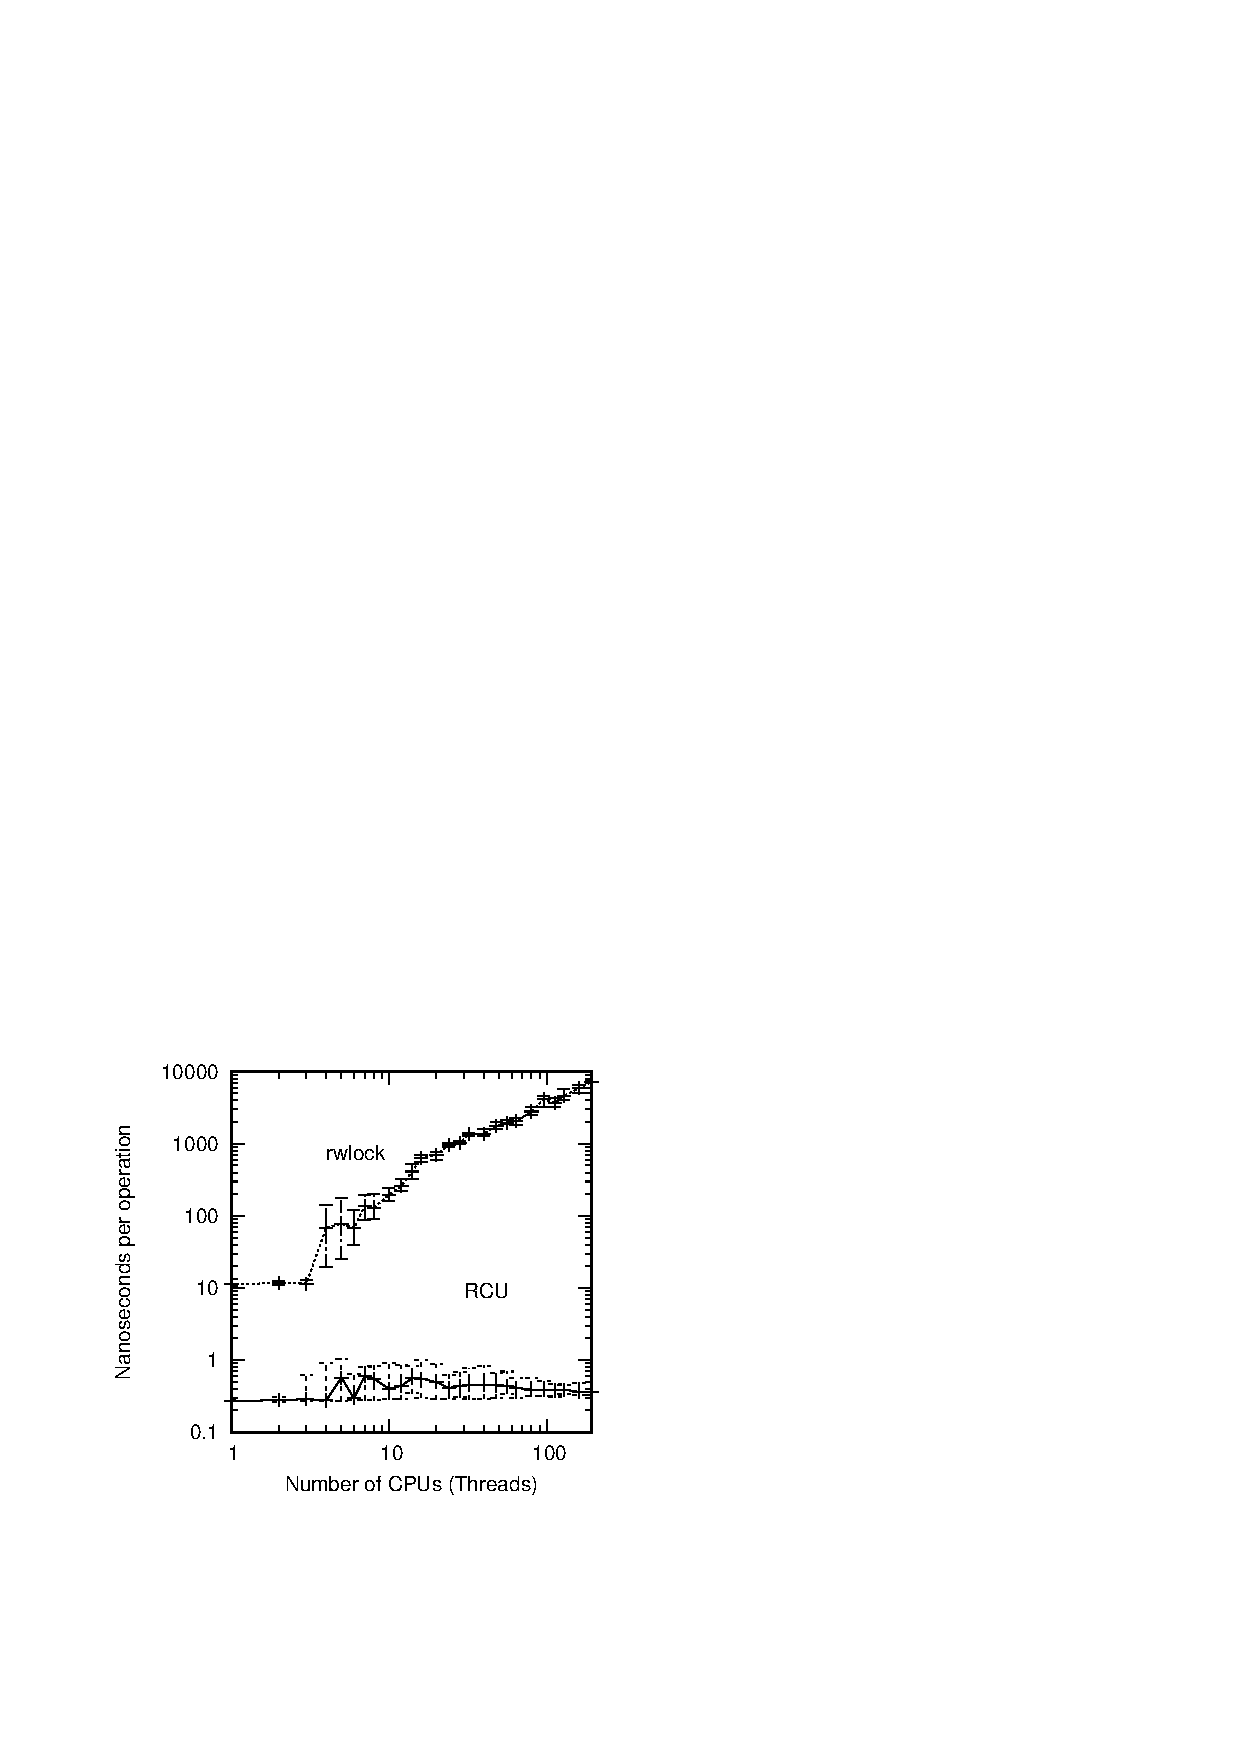
\includegraphics{defer/rwlockRCUperf}}
\caption{Performance Advantage of RCU Over Reader-Writer Locking}
\label{fig:defer:Performance Advantage of RCU Over Reader-Writer Locking}
\end{figure}

The read-side performance advantages of RCU over reader-writer locking
are shown in
Figure~\ref{fig:defer:Performance Advantage of RCU Over Reader-Writer Locking}.

\QuickQuiz{}
	WTF?
	How the heck do you expect me to believe that RCU has a
	100-femtosecond overhead when the clock period at 3\,GHz is more than
	300 \emph{picoseconds}?
\QuickQuizAnswer{
	First, consider that the inner loop used to
	take this measurement is as follows:

\vspace{5pt}
\begin{minipage}[t]{\columnwidth}
\scriptsize
\begin{verbatim}
  1 for (i = 0; i < CSCOUNT_SCALE; i++) {
  2   rcu_read_lock();
  3   rcu_read_unlock();
  4 }
\end{verbatim}
\end{minipage}
\vspace{5pt}

	Next, consider the effective definitions of \co{rcu_read_lock()}
	and \co{rcu_read_unlock()}:

\vspace{5pt}
\begin{minipage}[t]{\columnwidth}
\scriptsize
\begin{verbatim}
  1 #define rcu_read_lock()   do { } while (0)
  2 #define rcu_read_unlock() do { } while (0)
\end{verbatim}
\end{minipage}
\vspace{5pt}

	Consider also that the compiler does simple optimizations,
	allowing it to replace the loop with:

\vspace{5pt}
\begin{minipage}[t]{\columnwidth}
\scriptsize
\begin{verbatim}
i = CSCOUNT_SCALE;
\end{verbatim}
\end{minipage}
\vspace{5pt}

	So the ``measurement'' of 100 femtoseconds is simply the fixed
	overhead of the timing measurements divided by the number of
	passes through the inner loop containing the calls
	to \co{rcu_read_lock()} and \co{rcu_read_unlock()}.
	And therefore, this measurement really is in error, in fact,
	in error by an arbitrary number of orders of magnitude.
	As you can see by the definition of \co{rcu_read_lock()}
	and \co{rcu_read_unlock()} above, the actual overhead
	is precisely zero.

	It certainly is not every day that a timing measurement of
	100 femtoseconds turns out to be an overestimate!
} \QuickQuizEnd

Note that reader-writer locking is orders of magnitude slower than RCU
on a single CPU, and is almost two \emph{additional} orders of magnitude
slower on 16 CPUs.
In contrast, RCU scales quite well.
In both cases, the error bars span a single standard deviation in either
direction.

\begin{figure}[tb]
\centering
\resizebox{2.5in}{!}{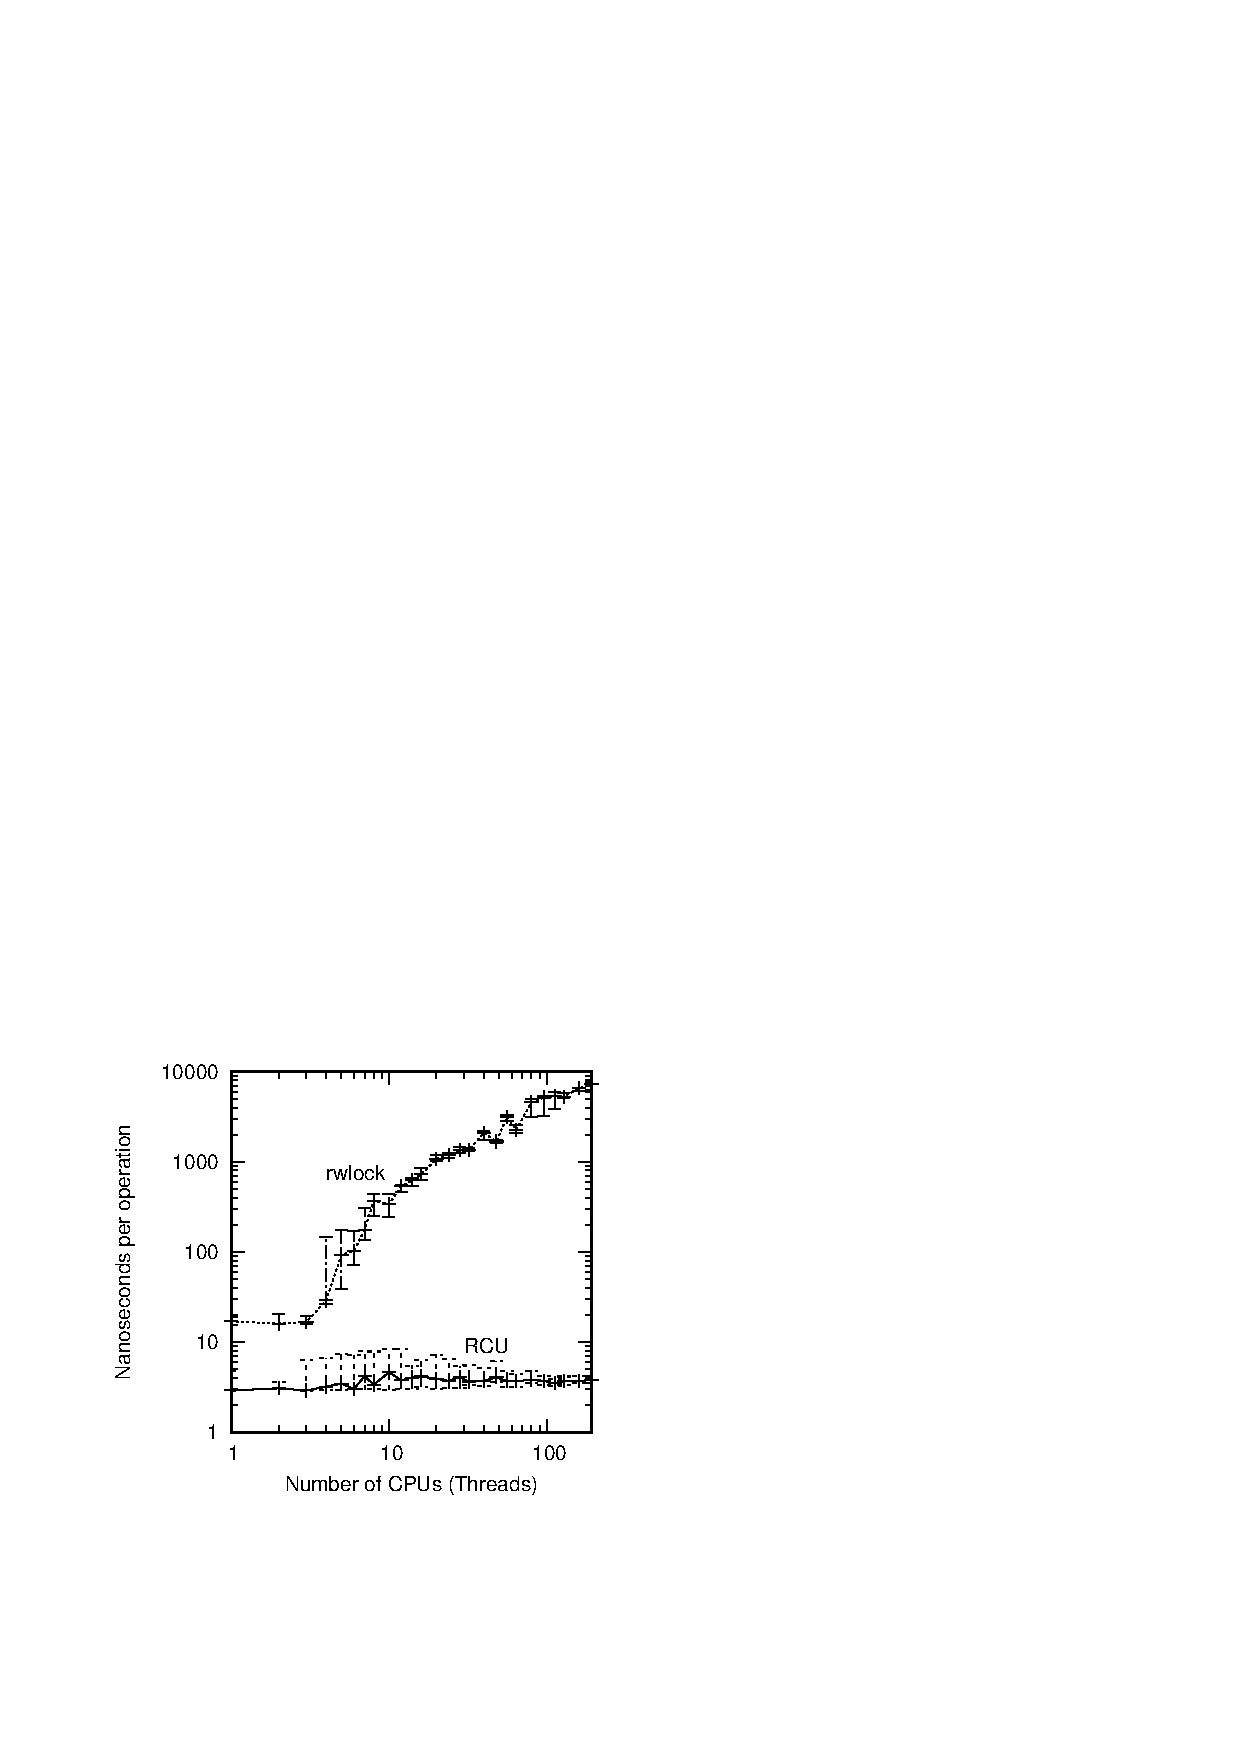
\includegraphics{defer/rwlockRCUperfPREEMPT}}
\caption{Performance Advantage of Preemptible RCU Over Reader-Writer Locking}
\label{fig:defer:Performance Advantage of Preemptible RCU Over Reader-Writer Locking}
\end{figure}

A more moderate view may be obtained from a \co{CONFIG_PREEMPT}
kernel, though RCU still beats reader-writer locking by between one and
three orders of magnitude, as shown in
Figure~\ref{fig:defer:Performance Advantage of Preemptible RCU Over Reader-Writer Locking}.
Note the high variability of reader-writer locking at larger numbers of CPUs.
The error bars span a single standard deviation in either direction.

\begin{figure}[tb]
\centering
\resizebox{2.5in}{!}{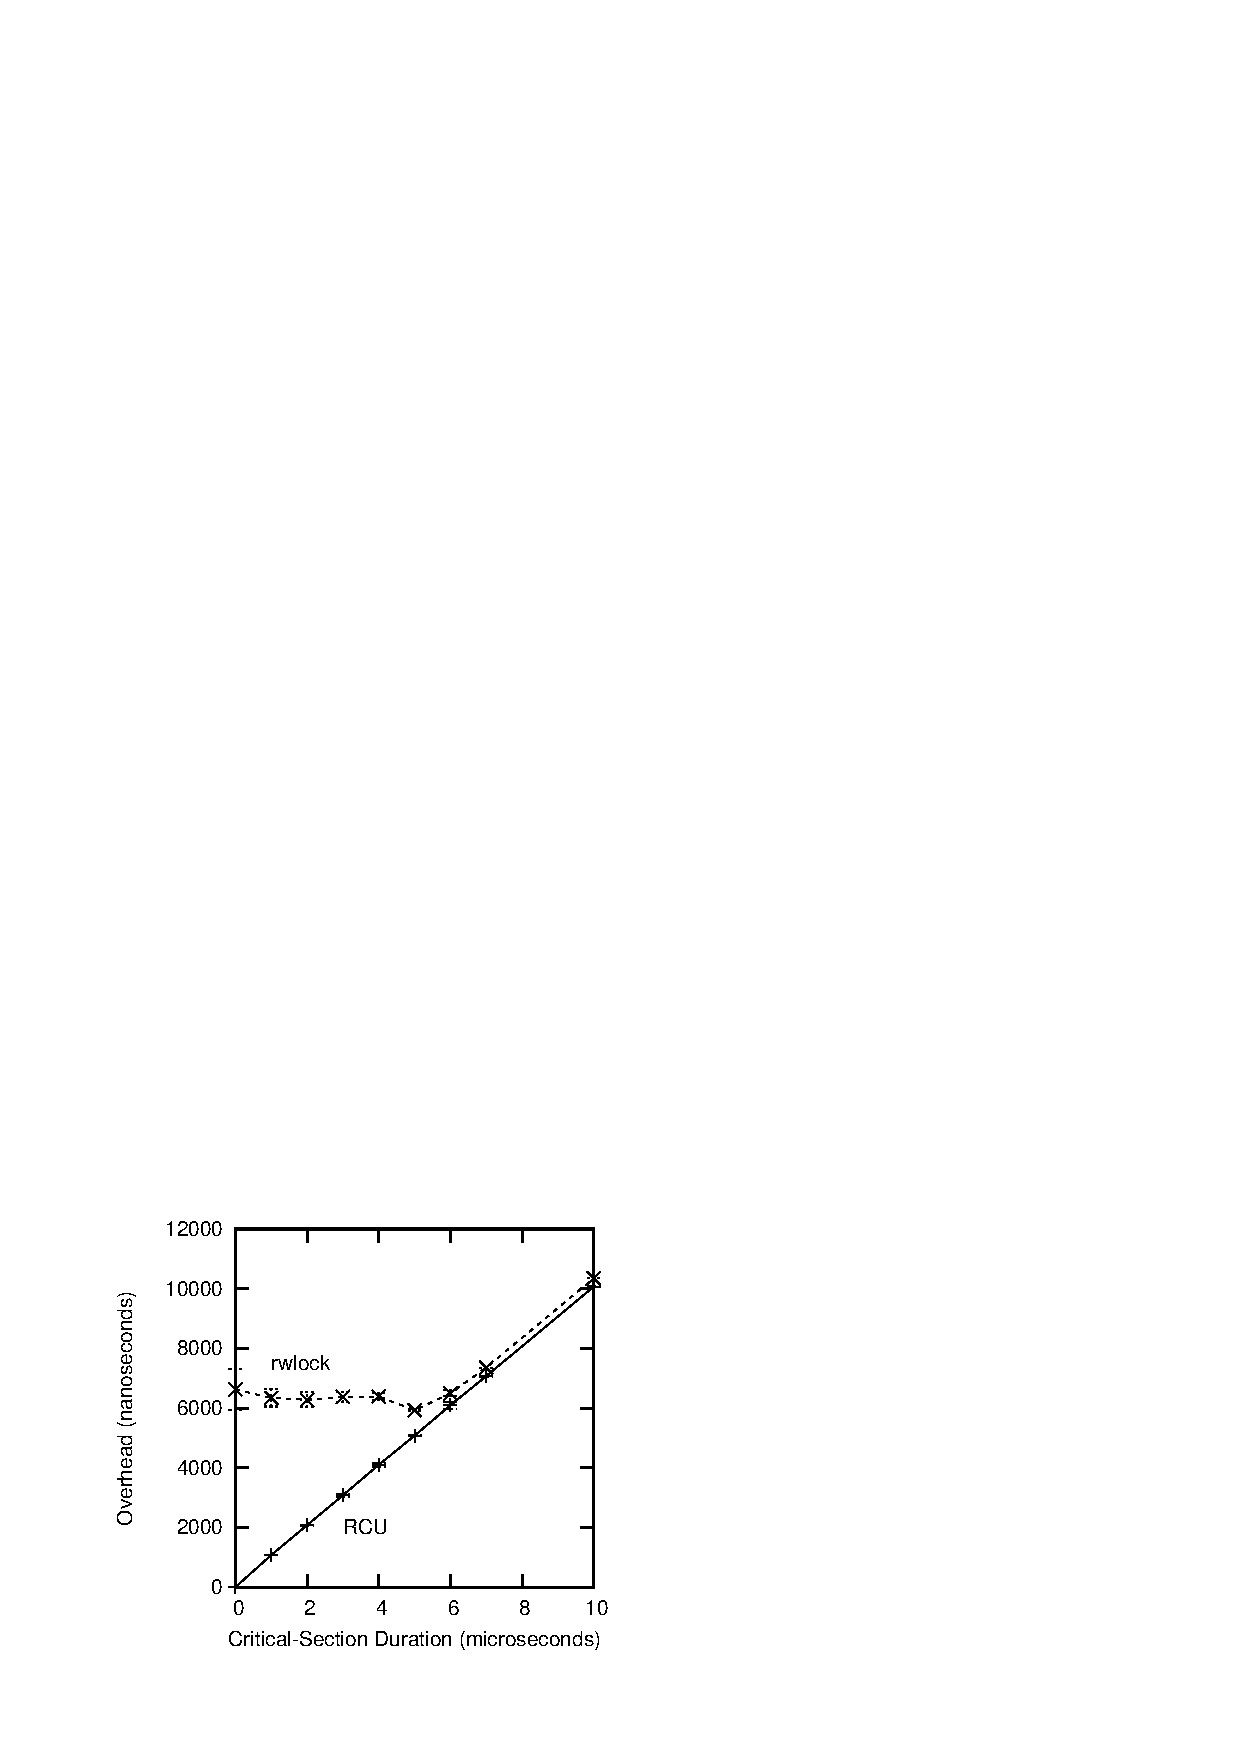
\includegraphics{defer/rwlockRCUperfwtPREEMPT}}
\caption{Comparison of RCU to Reader-Writer Locking as Function of Critical-Section Duration}
\label{fig:defer:Comparison of RCU to Reader-Writer Locking as Function of Critical-Section Duration}
\end{figure}

Of course, the low performance of reader-writer locking in
Figure~\ref{fig:defer:Performance Advantage of Preemptible RCU Over Reader-Writer Locking}
is exaggerated by the unrealistic zero-length critical sections.
The performance advantages of RCU become less significant as the overhead
of the critical section increases, as shown in
Figure~\ref{fig:defer:Comparison of RCU to Reader-Writer Locking as Function of Critical-Section Duration}
for a 16-CPU system,
in which the y-axis represents the sum of the overhead
of the read-side primitives and that of the critical section.

\QuickQuiz{}
	Why does both the variability and overhead of rwlock decrease as the
	critical-section overhead increases?
\QuickQuizAnswer{
	Because the contention on the underlying
	\co{rwlock_t} decreases as the critical-section overhead
	increases.
	However, the rwlock overhead will not quite drop to that on a single
	CPU because of cache-thrashing overhead.
} \QuickQuizEnd

However, this observation must be tempered by the fact that
a number of system calls (and thus any RCU read-side critical sections
that they contain) can complete within a few microseconds.

In addition, as is discussed in the next section,
RCU read-side primitives are almost entirely deadlock-immune.


\paragraph{Deadlock Immunity}

Although RCU offers significant performance advantages for
read-mostly workloads, one of the primary reasons for creating
RCU in the first place was in fact its immunity to read-side
deadlocks.
This immunity stems from the fact that
RCU read-side primitives do not block, spin, or even
do backwards branches, so that their execution time is deterministic.
It is therefore impossible for them to participate in a deadlock
cycle.

\QuickQuiz{}
	Is there an exception to this deadlock immunity, and if so,
	what sequence of events could lead to deadlock?
\QuickQuizAnswer{
	One way to cause a deadlock cycle involving
	RCU read-side primitives is via the following (illegal) sequence
	of statements:

\vspace{5pt}
\begin{minipage}[t]{\columnwidth}
\small
\begin{verbatim}
rcu_read_lock();
synchronize_rcu();
rcu_read_unlock();
\end{verbatim}
\end{minipage}
\vspace{5pt}

	The \co{synchronize_rcu()} cannot return until all
	pre-existing RCU read-side critical sections complete, but
	is enclosed in an RCU read-side critical section that cannot
	complete until the \co{synchronize_rcu()} returns.
	The result is a classic self-deadlock---you get the same
	effect when attempting to write-acquire a reader-writer lock
	while read-holding it.

	Note that this self-deadlock scenario does not apply to
	RCU QSBR, because the context switch performed by the
	\co{synchronize_rcu()} would act as a quiescent state
	for this CPU, allowing a grace period to complete.
	However, this is if anything even worse, because data used
	by the RCU read-side critical section might be freed as a
	result of the grace period completing.

	In short, do not invoke synchronous RCU update-side primitives
	from within an RCU read-side critical section.
} \QuickQuizEnd

An interesting consequence of RCU's read-side deadlock immunity is
that it is possible to unconditionally upgrade an RCU
reader to an RCU updater.
Attempting to do such an upgrade with reader-writer locking results
in deadlock.
A sample code fragment that does an RCU read-to-update upgrade follows:

\vspace{5pt}
\begin{minipage}[t]{\columnwidth}
\scriptsize
\begin{verbatim}
  1 rcu_read_lock();
  2 list_for_each_entry_rcu(p, &head, list_field) {
  3   do_something_with(p);
  4   if (need_update(p)) {
  5     spin_lock(my_lock);
  6     do_update(p);
  7     spin_unlock(&my_lock);
  8   }
  9 }
 10 rcu_read_unlock();
\end{verbatim}
\end{minipage}
\vspace{5pt}

Note that \co{do_update()} is executed under
the protection of the lock \emph{and} under RCU read-side protection.

Another interesting consequence of RCU's deadlock immunity is its
immunity to a large class of priority inversion problems.
For example, low-priority RCU readers cannot prevent a high-priority
RCU updater from acquiring the update-side lock.
Similarly, a low-priority RCU updater cannot prevent high-priority
RCU readers from entering an RCU read-side critical section.

\QuickQuiz{}
	Immunity to both deadlock and priority inversion???
	Sounds too good to be true.
	Why should I believe that this is even possible?
\QuickQuizAnswer{
	It really does work.
	After all, if it didn't work, the Linux kernel would not run.
} \QuickQuizEnd

\paragraph{Realtime Latency}

Because RCU read-side primitives neither spin nor block, they offer
excellent realtime latencies.
In addition, as noted earlier, this means that they are
immune to priority inversion
involving the RCU read-side primitives and locks.

However, RCU is susceptible to more subtle priority-inversion scenarios,
for example, a high-priority process blocked waiting for an RCU
grace period to elapse can be blocked by low-priority RCU readers
in -rt kernels.
This can be solved by using RCU priority
boosting~\cite{PaulEMcKenney2007BoostRCU,DinakarGuniguntala2008IBMSysJ}.

\paragraph{RCU Readers and Updaters Run Concurrently}

Because RCU readers never spin nor block, and because updaters are not
subject to any sort of rollback or abort semantics, RCU readers and
updaters must necessarily run concurrently.
This means that RCU readers might access stale data, and might even
see inconsistencies, either of which can render conversion from reader-writer
locking to RCU non-trivial.

\begin{figure}[tb]
\centering
\resizebox{3in}{!}{\includegraphics{defer/rwlockRCUupdate}}
\caption{Response Time of RCU vs. Reader-Writer Locking}
\label{fig:defer:Response Time of RCU vs. Reader-Writer Locking}
\end{figure}

However, in a surprisingly large number of situations, inconsistencies and
stale data are not problems.
The classic example is the networking routing table.
Because routing updates can take considerable time to reach a given
system (seconds or even minutes), the system will have been sending
packets the wrong way for quite some time when the update arrives.
It is usually not a problem to continue sending updates the wrong
way for a few additional milliseconds.
Furthermore, because RCU updaters can make changes without waiting for
RCU readers to finish,
the RCU readers might well see the change more quickly than would
batch-fair
reader-writer-locking readers, as shown in
Figure~\ref{fig:defer:Response Time of RCU vs. Reader-Writer Locking}.

Once the update is received, the rwlock writer cannot proceed until the
last reader completes, and subsequent readers cannot proceed until the
writer completes.
However, these subsequent readers are guaranteed to see the new value,
as indicated by the green shading of the rightmost boxes.
In contrast, RCU readers and updaters do not block each other, which permits
the RCU readers to see the updated values sooner.
Of course, because their execution overlaps that of the RCU updater,
\emph{all} of the RCU readers might well see updated values, including
the three readers that started before the update.
Nevertheless only the green-shaded rightmost RCU readers
are \emph{guaranteed} to see the updated values.

Reader-writer locking and RCU simply provide different guarantees.
With reader-writer locking, any reader that begins after the writer begins
is guaranteed to see new values, and any reader that attempts to
begin while the writer is spinning might or might not see new values,
depending on the reader/writer preference of the rwlock implementation in
question.
In contrast, with RCU, any reader that begins after the updater completes
is guaranteed to see new values, and any reader that completes after the
updater begins might or might not see new values, depending on timing.

The key point here is that, although reader-writer locking does
indeed guarantee consistency within the confines of the computer system,
there are situations where this consistency comes at the price of
increased \emph{inconsistency} with the outside world.
In other words, reader-writer locking obtains internal consistency at the
price of silently stale data with respect to the outside world.

Nevertheless, there are situations where inconsistency and stale
data within the confines of the system cannot be tolerated.
Fortunately,
there are a number of approaches that avoid inconsistency and stale
data~\cite{PaulEdwardMcKenneyPhD,Arcangeli03}, and some
methods based on reference counting are discussed in
Section~\ref{sec:defer:Reference Counting}.

\paragraph{Low-Priority RCU Readers Can Block High-Priority Reclaimers}

In Realtime RCU~\cite{DinakarGuniguntala2008IBMSysJ},
SRCU~\cite{PaulEMcKenney2006c}, or
QRCU~\cite{PaulEMcKenney2007QRCUspin} (see
Section~\ref{sec:formal:Promela Example: QRCU}),
a preempted reader will prevent
a grace period from completing, even if a high-priority task is
blocked waiting for that grace period to complete.
Realtime RCU can avoid this problem by substituting \co{call_rcu()}
for \co{synchronize_rcu()} or by using RCU priority
boosting~\cite{PaulEMcKenney2007BoostRCU,DinakarGuniguntala2008IBMSysJ},
which is still in experimental status as of early 2008.
It might become necessary to augment SRCU and QRCU with priority boosting,
but not before a clear real-world need is demonstrated.

\paragraph{RCU Grace Periods Extend for Many Milliseconds}

With the exception of QRCU and several of the ``toy'' RCU implementations
described in
Appendix~\ref{chp:app:``Toy'' RCU Implementations},
RCU grace periods extend for multiple milliseconds.
Although there are a number of techniques to render such long delays
harmless, including use of the asynchronous interfaces where available
(\co{call_rcu()} and \co{call_rcu_bh()}), this situation
is a major reason for the rule of thumb that RCU be used in read-mostly
situations.

\paragraph{Comparison of Reader-Writer Locking and RCU Code}

In the best case, the conversion from reader-writer locking to RCU
is quite simple, as shown in
Figures~\ref{fig:defer:Converting Reader-Writer Locking to RCU: Data},
\ref{fig:defer:Converting Reader-Writer Locking to RCU: Search},
and
\ref{fig:defer:Converting Reader-Writer Locking to RCU: Deletion},
all taken from
Wikipedia~\cite{WikipediaRCU}.

\begin{figure*}[htbp]
{ \scriptsize
\begin{verbbox}
 1 struct el {                           1 struct el {
 2   struct list_head lp;                2   struct list_head lp;
 3   long key;                           3   long key;
 4   spinlock_t mutex;                   4   spinlock_t mutex;
 5   int data;                           5   int data;
 6   /* Other data fields */             6   /* Other data fields */
 7 };                                    7 };
 8 DEFINE_RWLOCK(listmutex);             8 DEFINE_SPINLOCK(listmutex);
 9 LIST_HEAD(head);                      9 LIST_HEAD(head);
\end{verbbox}
}
\hspace*{0.9in}\OneColumnHSpace{-0.5in}
\theverbbox
\caption{Converting Reader-Writer Locking to RCU: Data}
\label{fig:defer:Converting Reader-Writer Locking to RCU: Data}
\end{figure*}

\begin{figure*}[htbp]
{ \scriptsize
\begin{verbbox}
 1 int search(long key, int *result)     1 int search(long key, int *result)
 2 {                                     2 {
 3   struct el *p;                       3   struct el *p;
 4                                       4
 5   read_lock(&listmutex);              5   rcu_read_lock();
 6   list_for_each_entry(p, &head, lp) { 6   list_for_each_entry_rcu(p, &head, lp) {
 7     if (p->key == key) {              7     if (p->key == key) {
 8       *result = p->data;              8       *result = p->data;
 9       read_unlock(&listmutex);        9       rcu_read_unlock();
10       return 1;                      10       return 1;
11     }                                11     }
12   }                                  12   }
13   read_unlock(&listmutex);           13   rcu_read_unlock();
14   return 0;                          14   return 0;
15 }                                    15 }
\end{verbbox}
}
\hspace*{0.9in}\OneColumnHSpace{-0.5in}
\theverbbox
\caption{Converting Reader-Writer Locking to RCU: Search}
\label{fig:defer:Converting Reader-Writer Locking to RCU: Search}
\end{figure*}

\begin{figure*}[htbp]
{ \scriptsize
\begin{verbbox}
 1 int delete(long key)                  1 int delete(long key)
 2 {                                     2 {
 3   struct el *p;                       3   struct el *p;
 4                                       4
 5   write_lock(&listmutex);             5   spin_lock(&listmutex);
 6   list_for_each_entry(p, &head, lp) { 6   list_for_each_entry(p, &head, lp) {
 7     if (p->key == key) {              7     if (p->key == key) {
 8       list_del(&p->lp);               8       list_del_rcu(&p->lp);
 9       write_unlock(&listmutex);       9       spin_unlock(&listmutex);
                                        10       synchronize_rcu();
10       kfree(p);                      11       kfree(p);
11       return 1;                      12       return 1;
12     }                                13     }
13   }                                  14   }
14   write_unlock(&listmutex);          15   spin_unlock(&listmutex);
15   return 0;                          16   return 0;
16 }                                    17 }
\end{verbbox}
}
\hspace*{0.9in}\OneColumnHSpace{-0.5in}
\theverbbox
\caption{Converting Reader-Writer Locking to RCU: Deletion}
\label{fig:defer:Converting Reader-Writer Locking to RCU: Deletion}
\end{figure*}

More-elaborate cases of replacing reader-writer locking with RCU
are beyond the scope of this document.

\subsubsection{RCU is a Restricted Reference-Counting Mechanism}
\label{sec:defer:RCU is a Restricted Reference-Counting Mechanism}

Because grace periods are not allowed to complete while
there is an RCU read-side critical section in progress,
the RCU read-side primitives may be used as a restricted
reference-counting mechanism.
For example, consider the following code fragment:

\vspace{5pt}
\begin{minipage}[t]{\columnwidth}
\scriptsize
\begin{verbatim}
  1 rcu_read_lock();  /* acquire reference. */
  2 p = rcu_dereference(head);
  3 /* do something with p. */
  4 rcu_read_unlock();  /* release reference. */
\end{verbatim}
\end{minipage}
\vspace{5pt}

The \co{rcu_read_lock()} primitive can be thought of as
acquiring a reference to \co{p}, because a grace period
starting after the \co{rcu_dereference()} assigns to \co{p}
cannot possibly end until after we reach the matching
\co{rcu_read_unlock()}.
This reference-counting scheme is restricted in that
we are not allowed to block in RCU read-side critical sections,
nor are we permitted to hand off an RCU read-side critical section
from one task to another.

Regardless of these restrictions,
the following code can safely delete \co{p}:

\vspace{5pt}
\begin{minipage}[t]{\columnwidth}
\scriptsize
\begin{verbatim}
  1 spin_lock(&mylock);
  2 p = head;
  3 rcu_assign_pointer(head, NULL);
  4 spin_unlock(&mylock);
  5 /* Wait for all references to be released. */
  6 synchronize_rcu();
  7 kfree(p);
\end{verbatim}
\end{minipage}
\vspace{5pt}

The assignment to \co{head} prevents any future references
to \co{p} from being acquired, and the \co{synchronize_rcu()}
waits for any previously acquired references to be released.

\QuickQuiz{}
	But wait!
	This is exactly the same code that might be used when thinking
	of RCU as a replacement for reader-writer locking!
	What gives?
\QuickQuizAnswer{
	This is an effect of the Law of Toy Examples:
	beyond a certain point, the code fragments look the same.
	The only difference is in how we think about the code.
	However, this difference can be extremely important.
	For but one example of the importance, consider that if we think
	of RCU as a restricted reference counting scheme, we would never
	be fooled into thinking that the updates would exclude the RCU
	read-side critical sections.

	It nevertheless is often useful to think of RCU as a replacement
	for reader-writer locking, for example, when you are replacing
	reader-writer locking with RCU.
} \QuickQuizEnd

Of course, RCU can also be combined with traditional reference counting,
as discussed in
Section~\ref{sec:together:Refurbish Reference Counting}.

\begin{figure}[tb]
\centering
\resizebox{2.5in}{!}{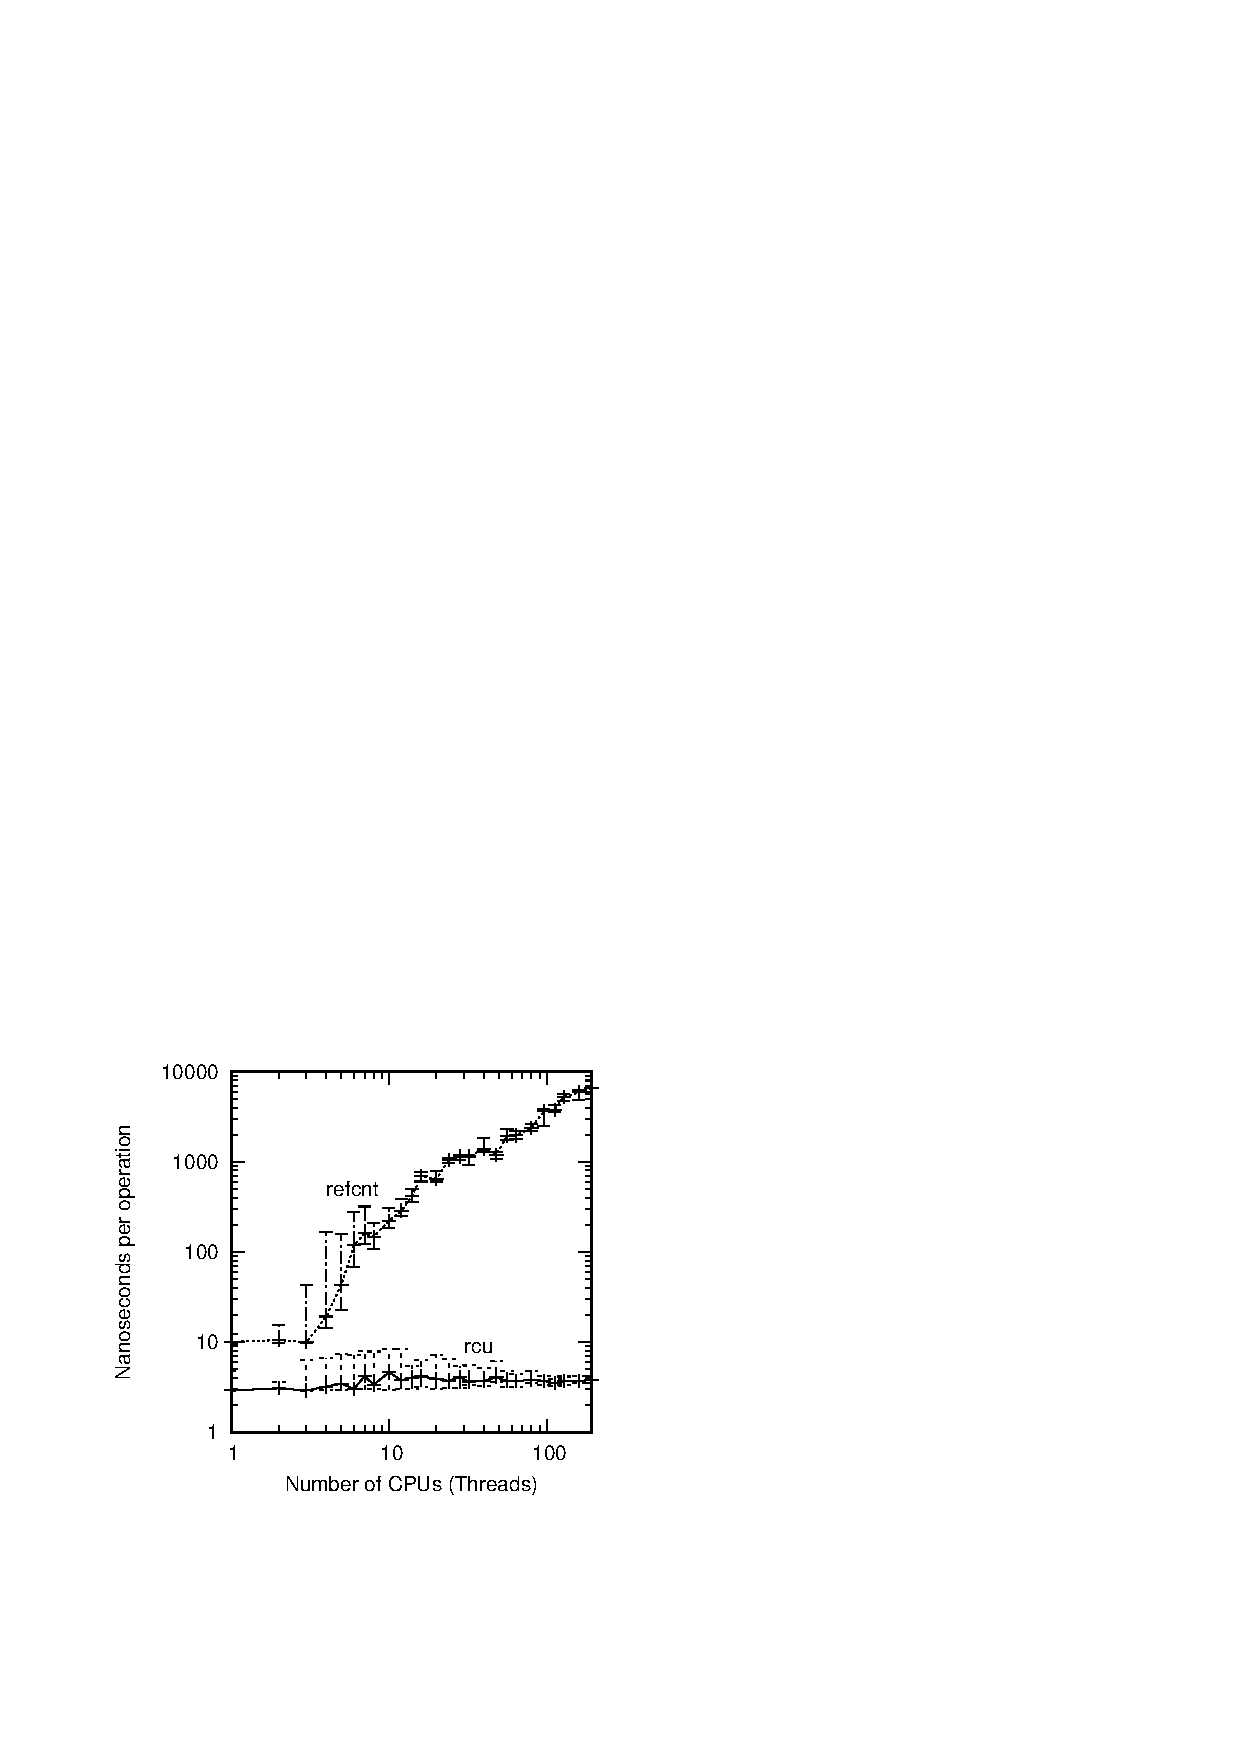
\includegraphics{defer/refRCUperfPREEMPT}}
\caption{Performance of RCU vs. Reference Counting}
\label{fig:defer:Performance of RCU vs. Reference Counting}
\end{figure}

But why bother?
Again, part of the answer is performance, as shown in
Figure~\ref{fig:defer:Performance of RCU vs. Reference Counting},
again showing data taken on a 16-CPU 3\,GHz Intel x86 system.

\QuickQuiz{}
	Why the dip in refcnt overhead near 6 CPUs?
\QuickQuizAnswer{
	Most likely NUMA effects.
	However, there is substantial variance in the values measured for the
	refcnt line, as can be seen by the error bars.
	In fact, standard deviations range in excess of 10\% of measured
	values in some cases.
	The dip in overhead therefore might well be a statistical aberration.
} \QuickQuizEnd

\begin{figure}[tb]
\centering
\resizebox{2.5in}{!}{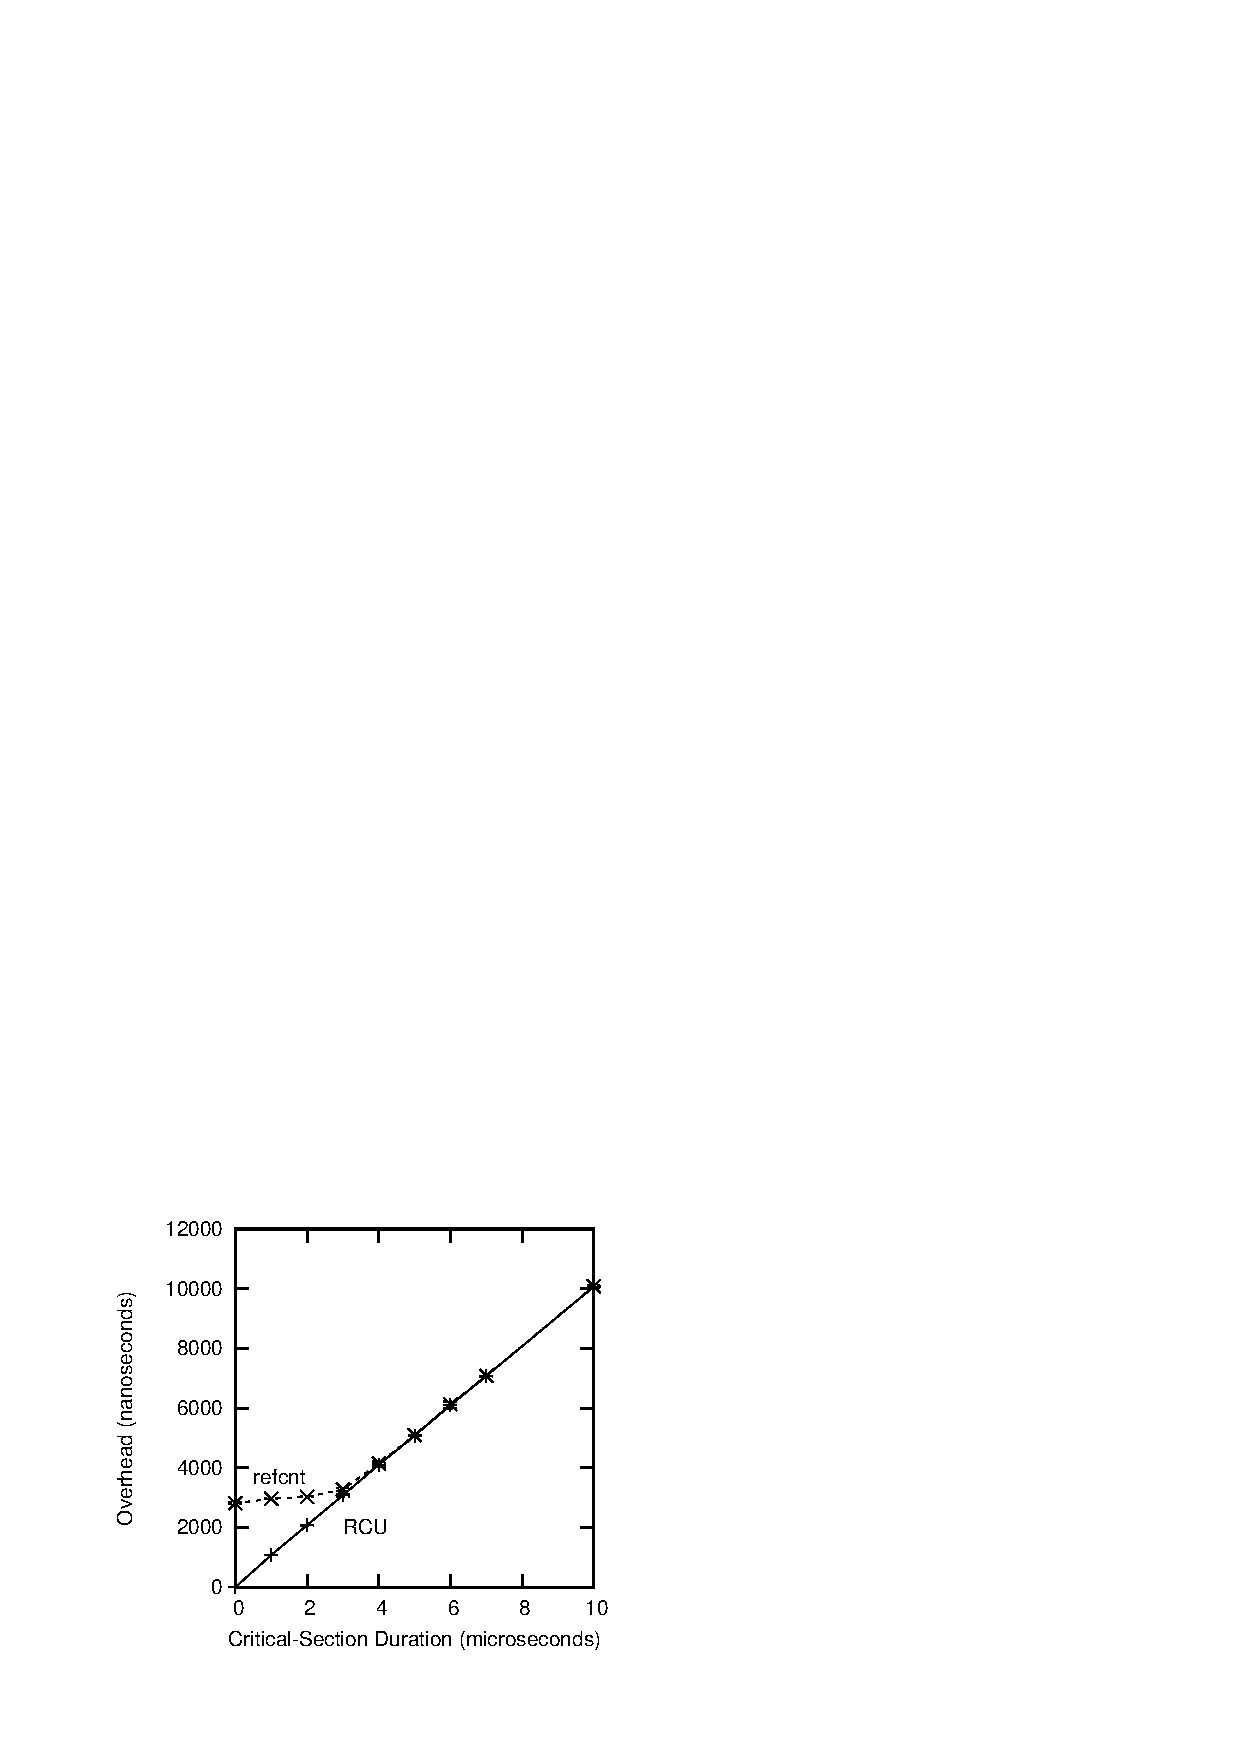
\includegraphics{defer/refRCUperfwtPREEMPT}}
\caption{Response Time of RCU vs. Reference Counting}
\label{fig:defer:Response Time of RCU vs. Reference Counting}
\end{figure}

And, as with reader-writer locking, the performance advantages
of RCU are most pronounced for short-duration critical sections, as shown
Figure~\ref{fig:defer:Response Time of RCU vs. Reference Counting}
for a 16-CPU system.
In addition, as with reader-writer locking, many system calls (and thus
any RCU read-side critical sections that they contain) complete in
a few microseconds.

However, the restrictions that go with RCU can be quite onerous.
For example, in many cases, the prohibition against sleeping while in an RCU
read-side critical section would defeat the entire purpose.
The next section looks at ways of addressing this problem, while also
reducing the complexity of traditional reference counting, at least in
some cases.

\subsubsection{RCU is a Bulk Reference-Counting Mechanism}
\label{sec:defer:RCU is a Bulk Reference-Counting Mechanism}

As noted in the preceding section,
traditional reference counters are usually associated with a specific
data structure, or perhaps a specific group of data structures.
However, maintaining a single global reference counter for a large
variety of data structures typically results in bouncing
the cache line containing the reference count.
Such cache-line bouncing can severely degrade performance.

In contrast, RCU's light-weight read-side primitives permit
extremely frequent read-side usage with negligible performance
degradation, permitting RCU to be used as a ``bulk reference-counting''
mechanism with little or no performance penalty.
Situations where a reference must be held by a single task across a
section of code that blocks may be accommodated with
Sleepable RCU (SRCU)~\cite{PaulEMcKenney2006c}.
This fails to cover the not-uncommon situation where a reference is ``passed''
from one task to another, for example, when a reference is acquired
when starting an I/O and released in the corresponding completion
interrupt handler.
(In principle, this could be handled by the SRCU implementation,
but in practice, it is not yet clear whether this is a good tradeoff.)

Of course, SRCU brings restrictions of its own, namely that the
return value from \co{srcu_read_lock()} be passed into the
corresponding \co{srcu_read_unlock()}, and that no SRCU primitives
be invoked from hardware interrupt handlers or from non-maskable interrupt
(NMI) handlers.
The jury is still out as to how much of a problem is presented by
these restrictions, and as to how they can best be handled.

\subsubsection{RCU is a Poor Man's Garbage Collector}
\label{sec:defer:RCU is a Poor Man's Garbage Collector}

A not-uncommon exclamation made by people first learning about
RCU is ``RCU is sort of like a garbage collector!''
This exclamation has a large grain of truth, but it can also be
misleading.

Perhaps the best way to think of the relationship between RCU
and automatic garbage collectors (GCs) is that RCU resembles
a GC in that the \emph{timing} of collection is automatically
determined, but that RCU differs from a GC in that: (1) the programmer
must manually indicate when a given data structure is eligible
to be collected, and (2) the programmer must manually mark the
RCU read-side critical sections where references might legitimately
be held.

Despite these differences, the resemblance does go quite deep,
and has appeared in at least one theoretical analysis of RCU.
Furthermore, the first RCU-like mechanism I am aware of used
a garbage collector to handle the grace periods.
Nevertheless, a better way of thinking of RCU is described in the
following section.

\subsubsection{RCU is a Way of Providing Existence Guarantees}
\label{sec:defer:RCU is a Way of Providing Existence Guarantees}

Gamsa et al.~\cite{Gamsa99}
discuss existence guarantees and describe how a mechanism
resembling RCU can be used to provide these existence guarantees
(see section~5 on page 7 of the PDF), and
Section~\ref{sec:locking:Lock-Based Existence Guarantees}
discusses how to guarantee existence via locking, along with the
ensuing disadvantages of doing so.
The effect is that if any RCU-protected data element is accessed
within an RCU read-side critical section, that data element is
guaranteed to remain in existence for the duration of that RCU
read-side critical section.

\begin{figure}[tbp]
{ \scriptsize
\begin{verbbox}
  1 int delete(int key)
  2 {
  3   struct element *p;
  4   int b;
  5 
  6   b = hashfunction(key);
  7   rcu_read_lock();
  8   p = rcu_dereference(hashtable[b]);
  9   if (p == NULL || p->key != key) {
 10     rcu_read_unlock();
 11     return 0;
 12   }
 13   spin_lock(&p->lock);
 14   if (hashtable[b] == p && p->key == key) {
 15     rcu_read_unlock();
 16     rcu_assign_pointer(hashtable[b], NULL);
 17     spin_unlock(&p->lock);
 18     synchronize_rcu();
 19     kfree(p);
 20     return 1;
 21   }
 22   spin_unlock(&p->lock);
 23   rcu_read_unlock();
 24   return 0;
 25 }
\end{verbbox}
}
\centering
\theverbbox
\caption{Existence Guarantees Enable Per-Element Locking}
\label{fig:defer:Existence Guarantees Enable Per-Element Locking}
\end{figure}

Figure~\ref{fig:defer:Existence Guarantees Enable Per-Element Locking}
demonstrates how RCU-based existence guarantees can enable
per-element locking via a function that deletes an element from
a hash table.
Line~6 computes a hash function, and line~7 enters an RCU
read-side critical section.
If line~9 finds that the corresponding bucket of the hash table is
empty or that the element present is not the one we wish to delete,
then line~10 exits the RCU read-side critical section and line~11
indicates failure.

\QuickQuiz{}
	What if the element we need to delete is not the first element
	of the list on line~9 of
	Figure~\ref{fig:defer:Existence Guarantees Enable Per-Element Locking}?
\QuickQuizAnswer{
	As with
	Figure~\ref{fig:locking:Per-Element Locking Without Existence Guarantees},
	this is a very simple hash table with no chaining, so the only
	element in a given bucket is the first element.
	The reader is again invited to adapt this example to a hash table with
	full chaining.
} \QuickQuizEnd

Otherwise, line~13 acquires the update-side spinlock, and
line~14 then checks that the element is still the one that we want.
If so, line~15 leaves the RCU read-side critical section,
line~16 removes it from the table, line~17 releases
the lock, line~18 waits for all pre-existing RCU read-side critical
sections to complete, line~19 frees the newly removed element,
and line~20 indicates success.
If the element is no longer the one we want, line~22 releases
the lock, line~23 leaves the RCU read-side critical section,
and line~24 indicates failure to delete the specified key.

\QuickQuiz{}
	Why is it OK to exit the RCU read-side critical section on
	line~15 of
	Figure~\ref{fig:defer:Existence Guarantees Enable Per-Element Locking}
	before releasing the lock on line~17?
\QuickQuizAnswer{
	First, please note that the second check on line~14 is
	necessary because some other
	CPU might have removed this element while we were waiting
	to acquire the lock.
	However, the fact that we were in an RCU read-side critical section
	while acquiring the lock guarantees that this element could not
	possibly have been re-allocated and re-inserted into this
	hash table.
	Furthermore, once we acquire the lock, the lock itself guarantees
	the element's existence, so we no longer need to be in an
	RCU read-side critical section.

	The question as to whether it is necessary to re-check the
	element's key is left as an exercise to the reader.
	% A re-check is necessary if the key can mutate or if it is
	% necessary to reject deleted entries (in cases where deletion
	% is recorded by mutating the key.
} \QuickQuizEnd

\QuickQuiz{}
	Why not exit the RCU read-side critical section on
	line~23 of
	Figure~\ref{fig:defer:Existence Guarantees Enable Per-Element Locking}
	before releasing the lock on line~22?
\QuickQuizAnswer{
	Suppose we reverse the order of these two lines.
	Then this code is vulnerable to the following sequence of
	events:
	\begin{enumerate}
	\item	CPU~0 invokes \co{delete()}, and finds the element
		to be deleted, executing through line~15.
		It has not yet actually deleted the element, but
		is about to do so.
	\item	CPU~1 concurrently invokes \co{delete()}, attempting
		to delete this same element.
		However, CPU~0 still holds the lock, so CPU~1 waits
		for it at line~13.
	\item	CPU~0 executes lines~16 and 17, and blocks at
		line~18 waiting for CPU~1 to exit its RCU read-side
		critical section.
	\item	CPU~1 now acquires the lock, but the test on line~14
		fails because CPU~0 has already removed the element.
		CPU~1 now executes line~22 (which we switched with line~23
		for the purposes of this Quick Quiz)
		and exits its RCU read-side critical section.
	\item	CPU~0 can now return from \co{synchronize_rcu()},
		and thus executes line~19, sending the element to
		the freelist.
	\item	CPU~1 now attempts to release a lock for an element
		that has been freed, and, worse yet, possibly
		reallocated as some other type of data structure.
		This is a fatal memory-corruption error.
	\end{enumerate}
} \QuickQuizEnd

Alert readers will recognize this as only a slight variation on
the original ``RCU is a way of waiting for things to finish'' theme,
which is addressed in
Section~\ref{sec:defer:RCU is a Way of Waiting for Things to Finish}.
They might also note the deadlock-immunity advantages over the lock-based
existence guarantees discussed in
Section~\ref{sec:locking:Lock-Based Existence Guarantees}.

\subsubsection{RCU is a Way of Providing Type-Safe Memory}
\label{sec:defer:RCU is a Way of Providing Type-Safe Memory}

A number of lockless algorithms do not require that a given data
element keep the same identity through a given RCU read-side critical
section referencing it---but only if that data element retains the
same type.
In other words, these lockless algorithms can tolerate a given data
element being freed and reallocated as the same type of structure
while they are referencing it, but must prohibit a change in type.
This guarantee, called ``type-safe memory'' in
academic literature~\cite{Cheriton96a},
is weaker than the existence guarantees in the
previous section, and is therefore quite a bit harder to work with.
Type-safe memory algorithms in the Linux kernel make use of slab caches,
specially marking these caches with \co{SLAB_DESTROY_BY_RCU}
so that RCU is used when returning a freed-up
slab to system memory.
This use of RCU guarantees that any in-use element of
such a slab will remain in that slab, thus retaining its type,
for the duration of any pre-existing RCU read-side critical sections.

\QuickQuiz{}
	But what if there is an arbitrarily long series of RCU
	read-side critical sections in multiple threads, so that at
	any point in time there is at least one thread in the system
	executing in an RCU read-side critical section?
	Wouldn't that prevent any data from a \co{SLAB_DESTROY_BY_RCU}
	slab ever being returned to the system, possibly resulting
	in OOM events?
\QuickQuizAnswer{
	There could certainly be an arbitrarily long period of time
	during which at least one thread is always in an RCU read-side
	critical section.
	However, the key words in the description in
	Section~\ref{sec:defer:RCU is a Way of Providing Type-Safe Memory}
	are ``in-use'' and ``pre-existing''.
	Keep in mind that a given RCU read-side critical section is
	conceptually only permitted to gain references to data elements
	that were in use at the beginning of that critical section.
	Furthermore, remember that a slab cannot be returned to the
	system until all of its data elements have been freed, in fact,
	the RCU grace period cannot start until after they have all been
	freed.

	Therefore, the slab cache need only wait for those RCU read-side
	critical sections that started before the freeing of the last element
	of the slab.
	This in turn means that any RCU grace period that begins after
	the freeing of the last element will do---the slab may be returned
	to the system after that grace period ends.
} \QuickQuizEnd

These algorithms typically use a validation step that checks to make
sure that the newly referenced data structure really is the one that
was requested~\cite[Section 2.5]{LaninShasha1986TSM}.
These validation checks require that portions of the data structure
remain untouched by the free-reallocate process.
Such validation checks are usually very hard to get right, and can
hide subtle and difficult bugs.

Therefore, although type-safety-based lockless algorithms can be extremely
helpful in a very few difficult situations, you should instead use existence
guarantees where possible.
Simpler is after all almost always better!

\subsubsection{RCU is a Way of Waiting for Things to Finish}
\label{sec:defer:RCU is a Way of Waiting for Things to Finish}

As noted in Section~\ref{sec:defer:RCU Fundamentals}
an important component
of RCU is a way of waiting for RCU readers to finish.
One of
RCU's great strengths is that it allows you to wait for each of
thousands of different things to finish without having to explicitly
track each and every one of them, and without having to worry about
the performance degradation, scalability limitations, complex deadlock
scenarios, and memory-leak hazards that are inherent in schemes that
use explicit tracking.

In this section, we will show how \co{synchronize_sched()}'s
read-side counterparts (which include anything that disables preemption,
along with hardware operations and
primitives that disable interrupts) permit you to implement interactions with
non-maskable interrupt
(NMI) handlers that would be quite difficult if using locking.
This approach has been called ``Pure RCU''~\cite{PaulEdwardMcKenneyPhD},
and it is used in a number of places in the Linux kernel.

The basic form of such ``Pure RCU'' designs is as follows:

\begin{enumerate}
\item	Make a change, for example, to the way that the OS reacts to an NMI.
\item	Wait for all pre-existing read-side critical sections to
	completely finish (for example, by using the
	\co{synchronize_sched()} primitive).
	The key observation here is that subsequent RCU read-side critical
	sections are guaranteed to see whatever change was made.
\item	Clean up, for example, return status indicating that the
	change was successfully made.
\end{enumerate}

The remainder of this section presents example code adapted from
the Linux kernel.
In this example, the \co{timer_stop} function uses
\co{synchronize_sched()} to ensure that all in-flight NMI
notifications have completed before freeing the associated resources.
A simplified version of this code is shown
Figure~\ref{fig:defer:Using RCU to Wait for NMIs to Finish}.

\begin{figure}[tbp]
{ \scriptsize
\begin{verbbox}
  1 struct profile_buffer {
  2   long size;
  3   atomic_t entry[0];
  4 };
  5 static struct profile_buffer *buf = NULL;
  6
  7 void nmi_profile(unsigned long pcvalue)
  8 {
  9   struct profile_buffer *p = rcu_dereference(buf);
 10
 11   if (p == NULL)
 12     return;
 13   if (pcvalue >= p->size)
 14     return;
 15   atomic_inc(&p->entry[pcvalue]);
 16 }
 17
 18 void nmi_stop(void)
 19 {
 20   struct profile_buffer *p = buf;
 21
 22   if (p == NULL)
 23     return;
 24   rcu_assign_pointer(buf, NULL);
 25   synchronize_sched();
 26   kfree(p);
 27 }
\end{verbbox}
}
\centering
\theverbbox
\caption{Using RCU to Wait for NMIs to Finish}
\label{fig:defer:Using RCU to Wait for NMIs to Finish}
\end{figure}

Lines~1-4 define a \co{profile_buffer} structure, containing a
size and an indefinite array of entries.
Line~5 defines a pointer to a profile buffer, which is
presumably initialized elsewhere to point to a dynamically allocated
region of memory.

Lines~7-16 define the \co{nmi_profile()} function,
which is called from within an NMI handler.
As such, it cannot be preempted, nor can it be interrupted by a normal
interrupts handler, however, it is still subject to delays due to cache misses,
ECC errors, and cycle stealing by other hardware threads within the same
core.
Line~9 gets a local pointer to the profile buffer using the
\co{rcu_dereference()} primitive to ensure memory ordering on
DEC Alpha, and
lines~11 and 12 exit from this function if there is no
profile buffer currently allocated, while lines~13 and 14
exit from this function if the \co{pcvalue} argument
is out of range.
Otherwise, line~15 increments the profile-buffer entry indexed
by the \co{pcvalue} argument.
Note that storing the size with the buffer guarantees that the
range check matches the buffer, even if a large buffer is suddenly
replaced by a smaller one.

Lines~18-27 define the \co{nmi_stop()} function,
where the caller is responsible for mutual exclusion (for example,
holding the correct lock).
Line~20 fetches a pointer to the profile buffer, and
lines~22 and 23 exit the function if there is no buffer.
Otherwise, line~24 \co{NULL}s out the profile-buffer pointer
(using the \co{rcu_assign_pointer()} primitive to maintain
memory ordering on weakly ordered machines),
and line~25 waits for an RCU Sched grace period to elapse,
in particular, waiting for all non-preemptible regions of code,
including NMI handlers, to complete.
Once execution continues at line~26, we are guaranteed that
any instance of \co{nmi_profile()} that obtained a
pointer to the old buffer has returned.
It is therefore safe to free the buffer, in this case using the
\co{kfree()} primitive.

\QuickQuiz{}
	Suppose that the \co{nmi_profile()} function was preemptible.
	What would need to change to make this example work correctly?
\QuickQuizAnswer{
	One approach would be to use
	\co{rcu_read_lock()} and \co{rcu_read_unlock()}
	in \co{nmi_profile()}, and to replace the
	\co{synchronize_sched()} with \co{synchronize_rcu()},
	perhaps as shown in
	Figure~\ref{fig:defer:Using RCU to Wait for Mythical Preemptible NMIs to Finish}.
%
\begin{figure}[tb]
{\scriptsize
\begin{verbbox}
  1 struct profile_buffer {
  2   long size;
  3   atomic_t entry[0];
  4 };
  5 static struct profile_buffer *buf = NULL;
  6
  7 void nmi_profile(unsigned long pcvalue)
  8 {
  9   struct profile_buffer *p;
 10
 11   rcu_read_lock();
 12   p = rcu_dereference(buf);
 13   if (p == NULL) {
 14     rcu_read_unlock();
 15     return;
 16   }
 17   if (pcvalue >= p->size) {
 18     rcu_read_unlock();
 19     return;
 20   }
 21   atomic_inc(&p->entry[pcvalue]);
 22   rcu_read_unlock();
 23 }
 24
 25 void nmi_stop(void)
 26 {
 27   struct profile_buffer *p = buf;
 28
 29   if (p == NULL)
 30     return;
 31   rcu_assign_pointer(buf, NULL);
 32   synchronize_rcu();
 33   kfree(p);
 34 }
\end{verbbox}
}
\centering
\theverbbox
\caption{Using RCU to Wait for Mythical Preemptible NMIs to Finish}
\label{fig:defer:Using RCU to Wait for Mythical Preemptible NMIs to Finish}
\end{figure}
%
} \QuickQuizEnd

In short, RCU makes it easy to dynamically switch among profile
buffers (you just \emph{try} doing this efficiently with atomic
operations, or at all with locking!).
However, RCU is normally used at a higher level of abstraction, as
was shown in the previous sections.

\subsubsection{RCU Usage Summary}
\label{sec:defer:RCU Usage Summary}

At its core, RCU is nothing more nor less than an API that provides:

\begin{enumerate}
\item	a publish-subscribe mechanism for adding new data,
\item	a way of waiting for pre-existing RCU readers to finish, and
\item	a discipline of maintaining multiple versions to permit change
	without harming or unduly delaying concurrent RCU readers.
\end{enumerate}

That said, it is possible to build higher-level constructs
on top of RCU, including the reader-writer-locking, reference-counting,
and existence-guarantee constructs listed in the earlier sections.
Furthermore, I have no doubt that the Linux community will continue to
find interesting new uses for RCU,
as well as for any of a number of other synchronization primitives.

\begin{figure}[tbh]
\centering
\resizebox{3in}{!}{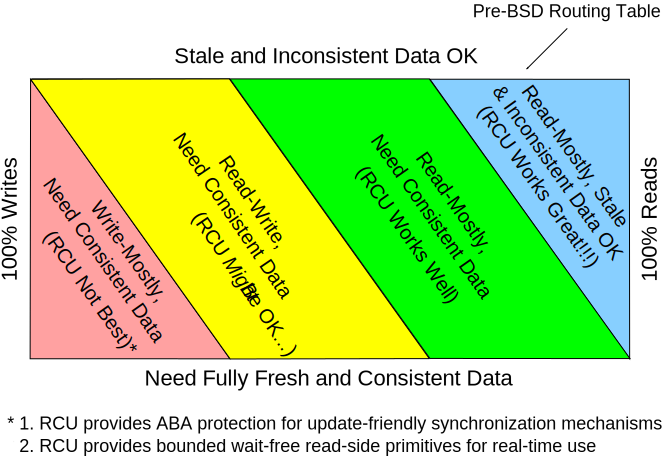
\includegraphics{defer/RCUApplicability}}
\caption{RCU Areas of Applicability}
\label{fig:defer:RCU Areas of Applicability}
\end{figure}

In the meantime,
Figure~\ref{fig:defer:RCU Areas of Applicability}
shows some rough rules of thumb on where RCU is most helpful.

As shown in the blue box at the top of the figure, RCU works best if
you have read-mostly data where stale and inconsistent
data is permissible (but see below for more information on stale and
inconsistent data).
The canonical example of this case in the Linux kernel is routing tables.
Because it may have taken many seconds or even minutes for the
routing updates to propagate across Internet, the system
has been sending packets the wrong way for quite some time.
Having some small probability of continuing to send some of them the wrong
way for a few more milliseconds is almost never a problem.

If you have a read-mostly workload where consistent data is required,
RCU works well, as shown by the green ``read-mostly, need consistent data''
box.
One example of this case is the Linux kernel's mapping from user-level
System-V semaphore IDs to the corresponding in-kernel data structures.
Semaphores tend to be used far more frequently than they are created
and destroyed, so this mapping is read-mostly.
However, it would be erroneous to perform a semaphore operation on
a semaphore that has already been deleted.
This need for consistency is handled by using the lock in the
in-kernel semaphore data structure, along with a ``deleted''
flag that is set when deleting a semaphore.
If a user ID maps to an in-kernel data structure with the
``deleted'' flag set, the data structure is ignored, so that
the user ID is flagged as invalid.

Although this requires that the readers acquire a lock for the
data structure representing the semaphore itself,
it allows them to dispense with locking for the
mapping data structure.
The readers therefore locklessly
traverse the tree used to map from ID to data structure,
which in turn greatly improves performance, scalability, and
real-time response.

As indicated by the yellow ``read-write'' box, RCU can also be useful
for read-write
workloads where consistent data is required, although usually in
conjunction with a number of other synchronization primitives.
For example, the directory-entry cache in recent Linux kernels uses RCU in
conjunction with sequence locks, per-CPU locks, and per-data-structure
locks to allow lockless traversal of pathnames in the common case.
Although RCU can be very beneficial in this read-write case, such
use is often more complex than that of the read-mostly cases.

Finally, as indicated by the red box at the bottom of the figure,
update-mostly workloads requiring
consistent data are rarely good places to use RCU, though there are some
exceptions~\cite{MathieuDesnoyers2012URCU}.
In addition, as noted in
Section~\ref{sec:defer:RCU is a Way of Providing Type-Safe Memory},
within the Linux kernel, the \co{SLAB_DESTROY_BY_RCU}
slab-allocator flag provides type-safe memory to RCU readers, which can
greatly simplify non-blocking synchronization and other lockless
algorithms.

In short, RCU is an API that includes a publish-subscribe mechanism for
adding new data, a way of waiting for pre-existing RCU readers to finish,
and a discipline of maintaining multiple versions to allow updates to
avoid harming or unduly delaying concurrent RCU readers.
This RCU API is best suited for read-mostly situations, especially if
stale and inconsistent data can be tolerated by the application.

% <h3>Acknowledgements</h3> @@@
%
% We are all indebted to Andy Whitcroft, Jon Walpole, and Gautham Shenoy,
% whose review of an early draft of this document greatly improved it.
% I owe thanks to the members of the Relativistic Programming project
% and to members of PNW TEC for many valuable discussions.
% I am grateful to Dan Frye for his support of this effort.

% defer/rcuAPI.tex

\subsection{RCU Linux-Kernel API}
\label{sec:defer:RCU Linux-Kernel API}
\OriginallyPublished{Section}{sec:defer:RCU Linux-Kernel API}{RCU Linux-Kernel API}{Linux Weekly News}{PaulEMcKenney2008WhatIsRCUAPI}

This section looks at RCU from the viewpoint of its Linux-kernel API.\footnote{
	Userspace RCU's API is documented
	elsewhere~\cite{PaulMcKenney2013LWNURCU}.}
Section~\ref{sec:defer:RCU has a Family of Wait-to-Finish APIs}
presents RCU's wait-to-finish APIs, and
Section~\ref{sec:defer:RCU has Publish-Subscribe and Version-Maintenance APIs}
presents RCU's publish-subscribe and version-maintenance APIs.
Finally,
Section~\ref{sec:defer:So, What is RCU Really?}
presents concluding remarks.

\subsubsection{RCU has a Family of Wait-to-Finish APIs}
\label{sec:defer:RCU has a Family of Wait-to-Finish APIs}

\begin{table*}[htbp]
\rowcolors{1}{}{lightgray}
\renewcommand*{\arraystretch}{1.3}
\centering
\caption{RCU Wait-to-Finish APIs}
\label{tab:defer:RCU Wait-to-Finish APIs}
\footnotesize
\begin{tabularx}{6.5in}{>{\raggedright\arraybackslash}p{1.08in}
    >{\raggedright\arraybackslash}X
    >{\raggedright\arraybackslash}X
    >{\raggedright\arraybackslash}p{1.3in}}
\toprule
Attribute &
    RCU &
	SRCU &
	    Tasks RCU \\
\midrule
Purpose &
    Original &
	Sleeping readers &
	    Free tracing trampolines \\
Read-side critical-section markers &
    \tco{rcu_read_lock()}~! \tco{rcu_read_unlock()}~!
    \tco{rcu_read_lock_bh()} \tco{rcu_read_unlock_bh()}
    \tco{rcu_read_lock_sched()} \tco{rcu_read_unlock_sched()}
    \tco{rcu_read_lock_sched_notrace()} \tco{rcu_read_unlock_sched_notrace()}
    (Plus anything disabing bottom halves, preemption, or interrupts.) &
	\tco{srcu_read_lock()} \tco{srcu_read_unlock()} &
	    Voluntary context switch \\
{ Update-side primitives (synchronous) } &
    { \tco{synchronize_rcu()} \tco{synchronize_rcu_expedited()}
      \tco{synchronize_net()} } &
	\tco{synchronize_srcu()} \tco{synchronize_srcu_expedited()} &
	    \tco{synchronize_rcu_tasks()} \\
{ Update-side primitives (asynchronous/callback) } &
    \tco{call_rcu()} ! &
	\tco{call_srcu()} &
	    \tco{call_rcu_tasks()} \\
{ Update-side primitives (wait for callbacks) } &
    \tco{rcu_barrier()} &
	\tco{srcu_barrier()} &
	    \tco{rcu_barrier_tasks()} \\
Type-safe memory &
    \tco{SLAB_DESTROY_BY_RCU} &
	&
	    \\
Read side constraints &
    No blocking (only preemption) &
	No \tco{synchronize_srcu()} with same \tco{srcu_struct} &
	    No voluntary context switch \\
Read side overhead &
    CPU-local accesses (free on \tco{PREEMPT=n}) &
	Simple instructions, memory barriers &
	    Free \\
Asynchronous update-side overhead &
    sub-microsecond &
	sub-microsecond &
	    sub-microsecond \\
Grace-period latency &
    10s of milliseconds &
        Milliseconds &
	    seconds \\
Expedited grace-period latency &
    10s of microseconds &
        Microseconds &
	    N/A \\
\bottomrule
\end{tabularx}
\end{table*}

The most straightforward answer to ``what is RCU'' is that RCU is
an API used in the Linux kernel, as summarized by
Table~\ref{tab:defer:RCU Wait-to-Finish APIs},
which shows the wait-for-readers portions of the RCU, ``sleepable'' RCU
(SRCU), Tasks RCU, and generic APIs, respectively,
and by
Table~\ref{tab:defer:RCU Publish-Subscribe and Version Maintenance APIs},
which shows the publish-subscribe portions of the API.
% @@@ Should the generic "Validation" APIs go elsewhere, thus allowing
% @@@ the "Generic" column to be removed?

% @@@ SRCU and Tasks RCU counterparts of "RCU API Usage Constraints" diagram?

% @@@ There are no special srcu list APIs.  Should there be?  Abstract somehow?

If you are new to RCU, you might consider focusing on just one
of the columns in
Table~\ref{tab:defer:RCU Wait-to-Finish APIs},
each of which summarizes one member of the Linux kernel's RCU API family.
For example, if you are primarily interested in understanding how RCU
is used in the Linux kernel, ``RCU Classic'' would be the place to start,
as it is used most frequently.
On the other hand, if you want to understand RCU for its own sake,
``SRCU'' has the simplest API.
You can always come back for the other columns later.

If you are already familiar with RCU, these tables can
serve as a useful reference.

\QuickQuiz{}
	Why do some of the cells in
	Table~\ref{tab:defer:RCU Wait-to-Finish APIs}
	have exclamation marks (``!'')?
\QuickQuizAnswer{
	The API members with exclamation marks (\co{rcu_read_lock()},
	\co{rcu_read_unlock()}, and \co{call_rcu()}) were the
	only members of the Linux RCU API that Paul E. McKenney was aware
	of back in the mid-90s.
	During this timeframe, he was under the mistaken impression that
	he knew all that there is to know about RCU.
} \QuickQuizEnd

The ``RCU Classic'' column corresponds to the original RCU implementation,
in which RCU read-side critical sections are delimited by
\co{rcu_read_lock()} and \co{rcu_read_unlock()}, which
may be nested.
The corresponding synchronous update-side primitives,
\co{synchronize_rcu()}, along with its synonym
\co{synchronize_net()}, wait for any currently executing
RCU read-side critical sections to complete.
The length of this wait is known as a ``grace period''.
The asynchronous update-side primitive, \co{call_rcu()},
invokes a specified function with a specified argument after a
subsequent grace period.
For example, \co{call_rcu(p,f);} will result in
the ``RCU callback'' \co{f(p)}
being invoked after a subsequent grace period.
There are situations,
such as when unloading a Linux-kernel module that uses \co{call_rcu()},
when it is necessary to wait for all
outstanding RCU callbacks to complete~\cite{PaulEMcKenney2007rcubarrier}.
The \co{rcu_barrier()} primitive does this job.
Note that the more recent hierarchical
RCU~\cite{PaulEMcKenney2008HierarchicalRCU}
implementation also adheres to ``RCU Classic'' semantics.

Finally, RCU may be used to provide
type-safe memory~\cite{Cheriton96a}, as described in
Section~\ref{sec:defer:RCU is a Way of Providing Type-Safe Memory}.
In the context of RCU, type-safe memory guarantees that a given
data element will not change type during any RCU read-side critical section
that accesses it.
To make use of RCU-based type-safe memory, pass
\co{SLAB_DESTROY_BY_RCU} to
\co{kmem_cache_create()}.
It is important to note that \co{SLAB_DESTROY_BY_RCU} will
\emph{in no way}
prevent \co{kmem_cache_alloc()} from immediately reallocating
memory that was just now freed via \co{kmem_cache_free()}!
In fact, the \co{SLAB_DESTROY_BY_RCU}-protected data structure
just returned by \co{rcu_dereference} might be freed and reallocated
an arbitrarily large number of times, even when under the protection
of \co{rcu_read_lock()}.
Instead, \co{SLAB_DESTROY_BY_RCU} operates by preventing
\co{kmem_cache_free()}
from returning a completely freed-up slab of data structures
to the system until after an RCU grace period elapses.
In short, although the data element might be freed and reallocated arbitrarily
often, at least its type will remain the same.

\QuickQuiz{}
	How do you prevent a huge number of RCU read-side critical
	sections from indefinitely blocking a \co{synchronize_rcu()}
	invocation?
\QuickQuizAnswer{
	There is no need to do anything to prevent RCU read-side
	critical sections from indefinitely blocking a
	\co{synchronize_rcu()} invocation, because the
	\co{synchronize_rcu()} invocation need wait only for
	\emph{pre-existing} RCU read-side critical sections.
	So as long as each RCU read-side critical section is
	of finite duration, there should be no problem.
} \QuickQuizEnd

\QuickQuiz{}
	The \co{synchronize_rcu()} API waits for all pre-existing
	interrupt handlers to complete, right?
\QuickQuizAnswer{
	Absolutely not!
	And especially not when using preemptible RCU!
	You instead want \co{synchronize_irq()}.
	Alternatively, you can place calls to \co{rcu_read_lock()}
	and \co{rcu_read_unlock()} in the specific interrupt handlers that
	you want \co{synchronize_rcu()} to wait for.
} \QuickQuizEnd

In the ``RCU BH'' column, \co{rcu_read_lock_bh()} and
\co{rcu_read_unlock_bh()} delimit RCU read-side critical
sections, \co{synchronize_rcu_bh()} waits for a grace period,
and \co{call_rcu_bh()} invokes the specified
function and argument after a later grace period.

\QuickQuiz{}
	What happens if you mix and match?
	For example, suppose you use \co{rcu_read_lock()} and
	\co{rcu_read_unlock()} to delimit RCU read-side critical
	sections, but then use \co{call_rcu_bh()} to post an
	RCU callback?
\QuickQuizAnswer{
	If there happened to be no RCU read-side critical
	sections delimited by \co{rcu_read_lock_bh()} and
	\co{rcu_read_unlock_bh()} at the time \co{call_rcu_bh()}
	was invoked, RCU would be within its rights to invoke the callback
	immediately, possibly freeing a data structure still being used by
	the RCU read-side critical section!
	This is not merely a theoretical possibility: a long-running RCU
	read-side critical section delimited by \co{rcu_read_lock()}
	and \co{rcu_read_unlock()} is vulnerable to this failure mode.

	However, the \co{rcu_dereference()} family of functions apply
	to all flavors of RCU.
	(There was an attempt to have per-flavor variants of
	\co{rcu_dereference()}, but it was just too messy.)
} \QuickQuizEnd

\QuickQuiz{}
	Hardware interrupt handlers can be thought of as being
	under the protection of an implicit \co{rcu_read_lock_bh()},
	right?
\QuickQuizAnswer{
	Absolutely not!
	And especially not when using preemptible RCU!
	If you need to access ``rcu\_bh''-protected data structures
	in an interrupt handler, you need to provide explicit calls to
	\co{rcu_read_lock_bh()} and \co{rcu_read_unlock_bh()}.
} \QuickQuizEnd

In the ``RCU Sched'' column, anything that disables preemption
acts as an RCU read-side critical section, and \co{synchronize_sched()}
waits for the corresponding RCU grace period.
This RCU API family was added in the 2.6.12 kernel, which split the
old \co{synchronize_kernel()} API into the current
\co{synchronize_rcu()} (for RCU Classic) and
\co{synchronize_sched()} (for RCU Sched).
Note that RCU Sched did not originally have an asynchronous
\co{call_rcu_sched()} interface, but one was added in 2.6.26.
In accordance with the quasi-minimalist philosophy of the Linux
community, APIs are added on an as-needed basis.

\QuickQuiz{}
	What happens if you mix and match RCU Classic and RCU Sched?
\QuickQuizAnswer{
	In a non-\co{PREEMPT} or a \co{PREEMPT} kernel, mixing these
	two works ``by accident'' because in those kernel builds, RCU Classic
	and RCU Sched map to the same implementation.
	However, this mixture is fatal in \co{PREEMPT_RT} builds using the -rt
	patchset, due to the fact that Realtime RCU's read-side critical
	sections can be preempted, which would permit
	\co{synchronize_sched()} to return before the
	RCU read-side critical section reached its \co{rcu_read_unlock()}
	call.
	This could in turn result in a data structure being freed before the
	read-side critical section was finished with it,
	which could in turn greatly increase the actuarial risk experienced
	by your kernel.

	In fact, the split between RCU Classic and RCU Sched was inspired
	by the need for preemptible RCU read-side critical sections.
} \QuickQuizEnd

\QuickQuiz{}
	In general, you cannot rely on \co{synchronize_sched()} to
	wait for all pre-existing interrupt handlers,
	right?
\QuickQuizAnswer{
	That is correct!
	Because -rt Linux uses threaded interrupt handlers, there can
	be context switches in the middle of an interrupt handler.
	Because \co{synchronize_sched()} waits only until each
	CPU has passed through a context switch, it can return
	before a given interrupt handler completes.

	If you need to wait for a given interrupt handler to complete,
	you should instead use \co{synchronize_irq()} or place
	explicit RCU read-side critical sections in the interrupt
	handlers that you wish to wait on.
} \QuickQuizEnd

The ``Realtime RCU'' column has the same API as does
RCU Classic, the only difference being that RCU read-side critical
sections may be preempted and may block while acquiring spinlocks.
The design of Realtime RCU is described
elsewhere~\cite{PaulEMcKenney2007PreemptibleRCU}.

The ``SRCU'' column in
Table~\ref{tab:defer:RCU Wait-to-Finish APIs}
displays a specialized RCU API that permits
general sleeping in RCU read-side critical
sections~\cite{PaulEMcKenney2006c}.
Of course,
use of \co{synchronize_srcu()} in an SRCU read-side
critical section can result in
self-deadlock, so should be avoided.
SRCU differs from earlier RCU implementations in that the caller
allocates an \co{srcu_struct} for each distinct SRCU
usage.
This approach prevents SRCU read-side critical sections from blocking
unrelated \co{synchronize_srcu()} invocations.
In addition, in this variant of RCU, \co{srcu_read_lock()}
returns a value that must be passed into the corresponding
\co{srcu_read_unlock()}.

\QuickQuiz{}
	Why should you be careful with \co{call_srcu()}?
\QuickQuizAnswer{
	A single task could register SRCU callbacks very quickly.
	Given that SRCU allows readers to block for arbitrary periods of
	time, this could consume an arbitrarily large quantity of memory.
	In contrast, given the synchronous \co{synchronize_srcu()}
	interface, a given task must finish waiting for a given grace period
	before it can start waiting for the next one.
} \QuickQuizEnd

\QuickQuiz{}
	Under what conditions can \co{synchronize_srcu()} be safely
	used within an SRCU read-side critical section?
\QuickQuizAnswer{
	In principle, you can use
	\co{synchronize_srcu()} with a given \co{srcu_struct}
	within an SRCU read-side critical section that uses some other
	\co{srcu_struct}.
	In practice, however, doing this is almost certainly a bad idea.
	In particular, the code shown in
	Listing~\ref{lst:defer:Multistage SRCU Deadlocks}
	could still result in deadlock.

\begin{listing}[htbp]
\begin{VerbatimL}
idx = srcu_read_lock(&ssa);
synchronize_srcu(&ssb);
srcu_read_unlock(&ssa, idx);

/* . . . */

idx = srcu_read_lock(&ssb);
synchronize_srcu(&ssa);
srcu_read_unlock(&ssb, idx);
\end{VerbatimL}
\caption{Multistage SRCU Deadlocks}
\label{lst:defer:Multistage SRCU Deadlocks}
\end{listing}
} \QuickQuizEnd

The Linux kernel currently has a surprising number of RCU APIs and
implementations.
There is some hope of reducing this number, evidenced by the fact
that a given build of the Linux kernel currently has at most
four implementations behind three APIs (given that RCU Classic
and Realtime RCU share the same API).
However, careful inspection and analysis will be required, just as
would be required in order to eliminate one of the many locking APIs.

The various RCU APIs are distinguished by the forward-progress
guarantees that their RCU read-side critical sections must provide,
and also by their scope, as follows:

\begin{enumerate}
\item	RCU BH: read-side critical sections
	must guarantee forward progress against everything except for
	NMI and interrupt handlers, but not including software-interrupt
	(\co{softirq}) handlers.
	RCU BH is global in scope.
\item	RCU Sched: read-side critical sections must guarantee forward
	progress against everything except for NMI and \IRQ\ handlers,
	including \co{softirq} handlers.
	RCU Sched is global in scope.
\item	RCU (both classic and real-time): read-side critical sections
	must guarantee forward progress against everything except for
	NMI handlers, \IRQ\ handlers, \co{softirq} handlers, and (in the
	real-time case) higher-priority real-time tasks.
	RCU is global in scope.
\item	SRCU: read-side critical sections need not guarantee
	forward progress unless some other task is waiting for the
	corresponding grace period to complete, in which case these
	read-side critical sections should complete in no more than
	a few seconds (and preferably much more quickly).\footnote{
		Thanks to James Bottomley for urging me to this
		formulation, as opposed to simply saying that
		there are no forward-progress guarantees.}
	SRCU's scope is defined by the use of the corresponding
	\co{srcu_struct}.
\end{enumerate}

In other words, SRCU compensate for their extremely weak
forward-progress guarantees by permitting the developer to restrict
their scope.

\subsubsection{RCU has Publish-Subscribe and Version-Maintenance APIs}
\label{sec:defer:RCU has Publish-Subscribe and Version-Maintenance APIs}

Fortunately, the RCU publish-subscribe and version-maintenance
primitives shown in
Table~\ref{tab:defer:RCU Publish-Subscribe and Version Maintenance APIs}
apply to all of the variants of RCU discussed above.
This commonality can in some cases allow more code to be shared,
which certainly reduces the API proliferation that would otherwise
occur.
The original purpose of the RCU publish-subscribe APIs was to
bury memory barriers into these APIs, so that Linux kernel
programmers could use RCU without needing to become expert on
the memory-ordering models of each of the 20+ CPU families
that Linux supports~\cite{Spraul01}.

\begin{table*}[tb]
\renewcommand*{\arraystretch}{1.15}
\footnotesize
\centering
\begin{tabular}{lllp{1.2in}}
\toprule
Category &
	Primitives &
		Availability &
			Overhead \\
\midrule
List traversal &
	\tco{list_for_each_entry_rcu()} &
		2.5.59 &
			Simple instructions (memory barrier on Alpha) \\
\midrule
List update &
	\tco{list_add_rcu()} &
		2.5.44 &
			Memory barrier \\
&
	\tco{list_add_tail_rcu()} &
		2.5.44 &
			Memory barrier \\
&
	\tco{list_del_rcu()} &
		2.5.44 &
			Simple instructions \\
&
	\tco{list_replace_rcu()} &
		2.6.9 &
			Memory barrier \\
&
	\tco{list_splice_init_rcu()} &
		2.6.21 &
			Grace-period latency \\
\midrule
Hlist traversal &
	\tco{hlist_for_each_entry_rcu()} &
		2.6.8 &
			Simple instructions (memory barrier on Alpha) \\
\midrule
Hlist update &
	\tco{hlist_add_behind_rcu()} &
		2.6.14 &
			Memory barrier \\
&	\multicolumn{2}{l}{(Renamed from \tco{hlist_add_after_rcu()} in 3.17)} &
			\\ \addlinespace[2pt]
&
	\tco{hlist_add_before_rcu()} &
		2.6.14 &
			Memory barrier \\
&
	\tco{hlist_add_head_rcu()} &
		2.5.64 &
			Memory barrier \\
&
	\tco{hlist_del_rcu()} &
		2.5.64 &
			Simple instructions \\
&
	\tco{hlist_replace_rcu()} &
		2.6.15 &
			Memory barrier \\
\midrule
Pointer traversal &
	\tco{rcu_dereference()} &
		2.6.9 &
			Simple instructions (memory barrier on Alpha) \\
\midrule
Pointer update &
	\tco{rcu_assign_pointer()} &
		2.6.10 &
			Memory barrier \\
\bottomrule
\end{tabular}
\caption{RCU Publish-Subscribe and Version Maintenance APIs}
\label{tab:defer:RCU Publish-Subscribe and Version Maintenance APIs}
\end{table*}

The first pair of categories operate on Linux
\co{struct list_head} lists, which are circular, doubly-linked
lists.
The \co{list_for_each_entry_rcu()} primitive traverses an
RCU-protected list in a type-safe manner, while also enforcing
memory ordering for situations where a new list element is inserted
into the list concurrently with traversal.
On non-Alpha platforms, this primitive incurs little or no performance
penalty compared to \co{list_for_each_entry()}.
The \co{list_add_rcu()}, \co{list_add_tail_rcu()},
and \co{list_replace_rcu()} primitives are analogous to
their non-RCU counterparts, but incur the overhead of an additional
memory barrier on weakly-ordered machines.
The \co{list_del_rcu()} primitive is also analogous to its
non-RCU counterpart, but oddly enough is very slightly faster due to the
fact that it poisons only the \co{prev} pointer rather than
both the \co{prev} and \co{next} pointers as
\co{list_del()} must do.
Finally, the \co{list_splice_init_rcu()} primitive is similar
to its non-RCU counterpart, but incurs a full grace-period latency.
The purpose of this grace period is to allow RCU readers to finish
their traversal of the source list before completely disconnecting
it from the list header---failure to do this could prevent such
readers from ever terminating their traversal.

\QuickQuiz{}
	Why doesn't \co{list_del_rcu()} poison both the \co{next}
	and \co{prev} pointers?
\QuickQuizAnswer{
	Poisoning the \co{next} pointer would interfere
	with concurrent RCU readers, who must use this pointer.
	However, RCU readers are forbidden from using the \co{prev}
	pointer, so it may safely be poisoned.
} \QuickQuizEnd

The second pair of categories operate on Linux's
\co{struct hlist_head}, which is a linear linked list.
One advantage of \co{struct hlist_head} over
\co{struct list_head} is that the former requires only
a single-pointer list header, which can save significant memory in
large hash tables.
The \co{struct hlist_head} primitives in the table
relate to their non-RCU counterparts in much the same way as do the
\co{struct list_head} primitives.

The final pair of categories operate directly on pointers, and
are useful for creating RCU-protected non-list data structures,
such as RCU-protected arrays and trees.
The \co{rcu_assign_pointer()} primitive ensures that any
prior initialization remains ordered before the assignment to the
pointer on weakly ordered machines.
Similarly, the \co{rcu_dereference()} primitive ensures that subsequent
code dereferencing the pointer will see the effects of initialization code
prior to the corresponding \co{rcu_assign_pointer()} on
Alpha CPUs.
On non-Alpha CPUs, \co{rcu_dereference()} documents which pointer
dereferences are protected by RCU.

\QuickQuiz{}
	Normally, any pointer subject to \co{rcu_dereference()} \emph{must}
	always be updated using \co{rcu_assign_pointer()}.
	What is an exception to this rule?
\QuickQuizAnswer{
	One such exception is when a multi-element linked
	data structure is initialized as a unit while inaccessible to other
	CPUs, and then a single \co{rcu_assign_pointer()} is used
	to plant a global pointer to this data structure.
	The initialization-time pointer assignments need not use
	\co{rcu_assign_pointer()}, though any such assignments that
	happen after the structure is globally visible \emph{must} use
	\co{rcu_assign_pointer()}.

	However, unless this initialization code is on an impressively hot
	code-path, it is probably wise to use \co{rcu_assign_pointer()}
	anyway, even though it is in theory unnecessary.
	It is all too easy for a ``minor'' change to invalidate your cherished
	assumptions about the initialization happening privately.
} \QuickQuizEnd

\QuickQuiz{}
	Are there any downsides to the fact that these traversal and update
	primitives can be used with any of the RCU API family members?
\QuickQuizAnswer{
	It can sometimes be difficult for automated
	code checkers such as ``sparse'' (or indeed for human beings) to
	work out which type of RCU read-side critical section a given
	RCU traversal primitive corresponds to.
	For example, consider the code shown in
	Listing~\ref{lst:defer:Diverse RCU Read-Side Nesting}.

\begin{listing}[htbp]
\begin{VerbatimL}
rcu_read_lock();
preempt_disable();
p = rcu_dereference(global_pointer);

/* . . . */

preempt_enable();
rcu_read_unlock();
\end{VerbatimL}
\caption{Diverse RCU Read-Side Nesting}
\label{lst:defer:Diverse RCU Read-Side Nesting}
\end{listing}

	Is the \co{rcu_dereference()} primitive in an RCU Classic
	or an RCU Sched critical section?
	What would you have to do to figure this out?
} \QuickQuizEnd

\subsubsection{RCU Has Diagnostic APIs}
\label{sec:defer:RCU Has Diagnostic APIs}

\begin{table}[tb]
\renewcommand*{\arraystretch}{1.15}
\footnotesize
\centering
\begin{tabular}{ll}
\toprule
Category &
	Primitives \\
\midrule
Mark RCU pointer &
	\tco{__rcu} \\
\midrule
Debug-object support &
	\tco{init_rcu_head()} \\
&	\tco{destroy_rcu_head()} \\
&	\tco{init_rcu_head_on_stack()} \\
&	\tco{destroy_rcu_head_on_stack()} \\
\midrule
Stall-warning control &
	\tco{rcu_cpu_stall_reset()} \\
\midrule
Callback checking &
	\tco{rcu_head_init()} \\
&	\tco{rcu_head_after_call_rcu()} \\
\midrule
lockdep support &
	\tco{rcu_read_lock_held()} \\
&	\tco{rcu_read_lock_bh_held()} \\
&	\tco{rcu_read_lock_sched_held()} \\
&	\tco{srcu_read_lock_held()} \\
&	\tco{rcu_is_watching()} \\
&	\tco{RCU_LOCKDEP_WARN()} \\
&	\tco{RCU_NONIDLE()} \\
&	\tco{rcu_sleep_check()} \\
\bottomrule
\end{tabular}
\caption{RCU Diagnostic APIs}
\label{tab:defer:RCU Diagnostic APIs}
\end{table}

Table~\ref{tab:defer:RCU Diagnostic APIs}
shows RCU's diagnostic APIs.

The \co{__rcu} marks an RCU-protected pointer, for example,
\qco{struct foo __rcu *p;}.
Pointers that might be passed to \co{rcu_dereference()} can be marked,
but pointers holding values returned from \co{rcu_dereference()}
should not be.
Providing these markings on variables, structure fields, function
parameters, and return values allows the Linux kernel's \co{sparse}
tool to detect situtations where RCU-protected pointers are
incorrectly accessed using plain C-language loads and stores.

Debug-object support is automatic for any \co{rcu_head} structures
that are part of a structure obtained from the Linux kernel's
memory allocators, but those building their own special-purpose
memory allocators can use \co{init_rcu_head()} and \co{destroy_rcu_head()}
at allocation and free time, respectively.
Those using \co{rcu_head} structures allocated on the function-call
stack (it happens!) may use \co{init_rcu_head_on_stack()}
before first use and \co{destroy_rcu_head_on_stack()} after last use,
but before returning from the function.
Debug-object support allows detection of bugs involving passing the
same \co{rcu_head} structure to \co{call_rcu()} and friends in
quick succession, which is the \co{call_rcu()} counterpart to the
infamous double-free class of bugs.

Stall-warning control is provided by \co{rcu_cpu_stall_reset()}, which
allows the caller to suppress RCU CPU stall warnings for the remainder
of the current grace period.
RCU CPU stall warnings help pinpoint situations where an RCU read-side
critical section runs for an excessive length of time, and it is useful
for things like kernel debuggers to be able to suppress them, for example,
when encountering a breakpoint.

Callback checking is provided by \co{rcu_head_init()} and
\co{rcu_head_after_call_rcu()}.
The former is invoked on an \co{rcu_head} structure before it is passed
to \co{call_rcu()}, and then \co{rcu_head_after_call_rcu()} will
check to see if the callback is has been invoked with the specified
function.

Support for lockdep~\cite{JonathanCorbet2006lockdep} includes
\co{rcu_read_lock_held()},
\co{rcu_read_lock_bh_held()},
\co{rcu_read_lock_sched_held()}, and
\co{srcu_read_lock_held()},
each of which returns \co{true} if invoked within the corresponding
type of RCU read-side critical section.

\QuickQuiz{}
	Why isn't there a \co{rcu_read_lock_tasks()} for Tasks RCU?
\QuickQuizAnswer{
	Because Tasks RCU does not have read-side markers.
	Instead, Tasks RCU read-side critical sections are
	bounded by voluntary context switches.
} \QuickQuizEnd

Because \co{rcu_read_lock()} cannot be used from the idle loop,
and because energy-efficiency concerns have caused the idle loop
to become quite ornate, \co{rcu_is_watching()} returns true if
invoked in a context where use of \co{rcu_read_lock()} is legal.
Note again that \co{srcu_read_lock()} may be used from idle and
even offline CPUs, which means that \co{rcu_is_watching()} does not
apply to SRCU.

\co{RCU_LOCKDEP_WARN()} emits a warning if lockdep is enabled and if
its argument evaluated to \co{true}.
For example, \co{RCU_LOCKDEP_WARN(!rcu_read_lock_held())} would emit a
warning if invoked outside of an RCU read-side critical section.

\co{RCU_NONIDLE()} may be used to force RCU to watch when executing
the statement that is passed in as the sole argument.
For example, \co{RCU_NONIDLE(WARN_ON(!rcu_is_watching()))}
would never emit a warning.

Finally,  \co{rcu_sleep_check()} emits a warning if invoked within
an RCU, RCU-bh, or RCU-sched read-side critical section.

\subsubsection{Where Can RCU's APIs Be Used?}
\label{sec:defer:Where Can RCU's APIs Be Used?}

\begin{figure}[tb]
\centering
\resizebox{3in}{!}{\includegraphics{defer/RCUenvAPI}}
\caption{RCU API Usage Constraints}
\label{fig:defer:RCU API Usage Constraints}
\end{figure}

Figure~\ref{fig:defer:RCU API Usage Constraints}
shows which APIs may be used in which in-kernel environments.
The RCU read-side primitives may be used in any environment, including NMI,
the RCU mutation and asynchronous grace-period primitives may be used in any
environment other than NMI, and, finally, the RCU synchronous grace-period
primitives may be used only in process context.
The RCU list-traversal primitives include \co{list_for_each_entry_rcu()},
\co{hlist_for_each_entry_rcu()}, etc.
Similarly, the RCU list-mutation primitives include
\co{list_add_rcu()}, \co{hlist_del_rcu()}, etc.

Note that primitives from other families of RCU may be substituted,
for example, \co{srcu_read_lock()} may be used in any context
in which \co{rcu_read_lock()} may be used.

\subsubsection{So, What \emph{is} RCU Really?}
\label{sec:defer:So, What is RCU Really?}

At its core, RCU is nothing more nor less than an API that supports
publication and subscription for insertions, waiting for all RCU readers
to complete, and maintenance of multiple versions.
That said, it is possible to build higher-level constructs
on top of RCU, including the reader-writer-locking, reference-counting,
and existence-guarantee constructs listed in
Section~\ref{sec:defer:RCU Usage}.
Furthermore, I have no doubt that the Linux community will continue to
find interesting new uses for RCU,
just as they do for any of a number of synchronization
primitives throughout the kernel.

Of course, a more-complete view of RCU would also include
all of the things you can do with these APIs.

However, for many people, a complete view of RCU must include sample
RCU implementations.
Appendix~\ref{chp:app:``Toy'' RCU Implementations} therefore presents a series
of ``toy'' RCU implementations of increasing complexity and capability,
though others might prefer the classic
``User-Level Implementations of Read-Copy
Update''~\cite{MathieuDesnoyers2012URCU}.
For everyone else, the next section gives an overview of some RCU use cases.

% % defer/toyrcu.tex

\subsection{``Toy'' RCU Implementations}
\label{sec:defer:``Toy'' RCU Implementations}

The toy RCU implementations in this section are designed not for
high performance, practicality, or any kind of production use,\footnote{
	However, production-quality user-level RCU implementations
	are available~\cite{MathieuDesnoyers2009URCU}.}
but rather for clarity.
Nevertheless, you will need a thorough understanding of
Chapters~\ref{chp:Introduction},
\ref{chp:Hardware and its Habits},
\ref{chp:Tools of the Trade}, and
\ref{cha:Partitioning and Synchronization Design},
as well as the previous portions of
Chapter~\ref{chp:Deferred Processing}
for even these toy RCU implementations to be easily understandable.

This section provides a series of RCU implementations in order of
increasing sophistication, from the viewpoint of solving the
existence-guarantee problem.
Section~\ref{defer:Lock-Based RCU} presents a rudimentary
RCU implementation based on simple locking, while
Sections~\ref{defer:Per-Thread Lock-Based RCU} through
\ref{defer:RCU Based on Quiescent States}
present a series of
simple RCU implementations based on locking, reference counters,
and free-running counters.
Finally, Section~\ref{defer:Summary of Toy RCU Implementations}
provides a summary and a list of desirable RCU properties.

\subsubsection{Lock-Based RCU}
\label{defer:Lock-Based RCU}

\begin{figure}[bp]
{ \scriptsize
\begin{verbbox}
  1 static void rcu_read_lock(void)
  2 {
  3   spin_lock(&rcu_gp_lock);
  4 }
  5
  6 static void rcu_read_unlock(void)
  7 {
  8   spin_unlock(&rcu_gp_lock);
  9 }
 10
 11 void synchronize_rcu(void)
 12 {
 13   spin_lock(&rcu_gp_lock);
 14   spin_unlock(&rcu_gp_lock);
 15 }
\end{verbbox}
}
\centering
\theverbbox
\caption{Lock-Based RCU Implementation}
\label{fig:defer:Lock-Based RCU Implementation}
\end{figure}

Perhaps the simplest RCU implementation leverages locking, as
shown in
Figure~\ref{fig:defer:Lock-Based RCU Implementation}
(\path{rcu_lock.h} and \path{rcu_lock.c}).
In this implementation, \co{rcu_read_lock()} acquires a global
spinlock, \co{rcu_read_unlock()} releases it, and
\co{synchronize_rcu()} acquires it then immediately releases it.

Because \co{synchronize_rcu()} does not return until it has acquired
(and released) the lock, it cannot return until all prior RCU read-side
critical sections have completed, thus faithfully implementing
RCU semantics.
Of course, only one RCU reader may be in its read-side critical section
at a time, which almost entirely defeats the purpose of RCU.
In addition, the lock operations in \co{rcu_read_lock()} and
\co{rcu_read_unlock()} are extremely heavyweight,
with read-side overhead ranging from about 100~nanoseconds on a single Power5
CPU up to more than 17~\emph{microseconds} on a 64-CPU system.
Worse yet,
these same lock operations permit \co{rcu_read_lock()}
to participate in deadlock cycles.
Furthermore, in absence of recursive locks,
RCU read-side critical sections cannot be nested, and, finally,
although concurrent RCU updates could in principle be satisfied by
a common grace period, this implementation serializes grace periods,
preventing grace-period sharing.

\QuickQuiz{}
	Why wouldn't any deadlock in the RCU implementation in
	Figure~\ref{fig:defer:Lock-Based RCU Implementation}
	also be a deadlock in any other RCU implementation?
\QuickQuizAnswer{
%
\begin{figure}[tbp]
{ \scriptsize
\begin{verbbox}
  1 void foo(void)
  2 {
  3   spin_lock(&my_lock);
  4   rcu_read_lock();
  5   do_something();
  6   rcu_read_unlock();
  7   do_something_else();
  8   spin_unlock(&my_lock);
  9 }
 10
 11 void bar(void)
 12 {
 13   rcu_read_lock();
 14   spin_lock(&my_lock);
 15   do_some_other_thing();
 16   spin_unlock(&my_lock);
 17   do_whatever();
 18   rcu_read_unlock();
 19 }
\end{verbbox}
}
\centering
\theverbbox
\caption{Deadlock in Lock-Based RCU Implementation}
\label{fig:defer:Deadlock in Lock-Based RCU Implementation}
\end{figure}
%
	Suppose the functions \co{foo()} and \co{bar()} in
	Figure~\ref{fig:defer:Deadlock in Lock-Based RCU Implementation}
	are invoked concurrently from different CPUs.
	Then \co{foo()} will acquire \co{my_lock()} on line~3,
	while \co{bar()} will acquire \co{rcu_gp_lock} on
	line~13.
	When \co{foo()} advances to line~4, it will attempt to
	acquire \co{rcu_gp_lock}, which is held by \co{bar()}.
	Then when \co{bar()} advances to line~14, it will attempt
	to acquire \co{my_lock}, which is held by \co{foo()}.

	Each function is then waiting for a lock that the other
	holds, a classic deadlock.

	Other RCU implementations neither spin nor block in
	\co{rcu_read_lock()}, hence avoiding deadlocks.
} \QuickQuizEnd

\QuickQuiz{}
	Why not simply use reader-writer locks in the RCU implementation
	in
	Figure~\ref{fig:defer:Lock-Based RCU Implementation}
	in order to allow RCU readers to proceed in parallel?
\QuickQuizAnswer{
	One could in fact use reader-writer locks in this manner.
	However, textbook reader-writer locks suffer from memory
	contention, so that the RCU read-side critical sections would
	need to be quite long to actually permit parallel
	execution~\cite{McKenney03a}.

	On the other hand, use of a reader-writer lock that is
	read-acquired in \co{rcu_read_lock()} would avoid the
	deadlock condition noted above.
} \QuickQuizEnd

It is hard to imagine this implementation being useful
in a production setting, though it does have the virtue
of being implementable in almost any user-level application.
Furthermore, similar implementations having one lock per CPU
or using reader-writer locks have been used in production
in the 2.4 Linux kernel.

A modified version of this one-lock-per-CPU approach, but instead using
one lock per thread, is described
in the next section.

\subsubsection{Per-Thread Lock-Based RCU}
\label{defer:Per-Thread Lock-Based RCU}

\begin{figure}[tbp]
{ \scriptsize
\begin{verbbox}
  1 static void rcu_read_lock(void)
  2 {
  3   spin_lock(&__get_thread_var(rcu_gp_lock));
  4 }
  5
  6 static void rcu_read_unlock(void)
  7 {
  8   spin_unlock(&__get_thread_var(rcu_gp_lock));
  9 }
 10
 11 void synchronize_rcu(void)
 12 {
 13   int t;
 14
 15   for_each_running_thread(t) {
 16     spin_lock(&per_thread(rcu_gp_lock, t));
 17     spin_unlock(&per_thread(rcu_gp_lock, t));
 18   }
 19 }
\end{verbbox}
}
\centering
\theverbbox
\caption{Per-Thread Lock-Based RCU Implementation}
\label{fig:defer:Per-Thread Lock-Based RCU Implementation}
\end{figure}

Figure~\ref{fig:defer:Per-Thread Lock-Based RCU Implementation}
(\path{rcu_lock_percpu.h} and \path{rcu_lock_percpu.c})
shows an implementation based on one lock per thread.
The \co{rcu_read_lock()} and \co{rcu_read_unlock()} functions
acquire and release, respectively, the current thread's lock.
The \co{synchronize_rcu()} function acquires and releases each thread's
lock in turn.
Therefore, all RCU read-side critical sections running
when \co{synchronize_rcu()} starts must have completed before
\co{synchronize_rcu()} can return.

This implementation does have the virtue of permitting concurrent
RCU readers, and does avoid the deadlock condition that can arise
with a single global lock.
Furthermore, the read-side overhead, though high at roughly 140 nanoseconds,
remains at about 140 nanoseconds regardless of the number of CPUs.
However, the update-side overhead ranges from about 600 nanoseconds
on a single Power5 CPU
up to more than 100 \emph{microseconds} on 64 CPUs.

\QuickQuiz{}
	Wouldn't it be cleaner to acquire all the locks, and then
	release them all in the loop from lines~15-18 of
	Figure~\ref{fig:defer:Per-Thread Lock-Based RCU Implementation}?
	After all, with this change, there would be a point in time
	when there were no readers, simplifying things greatly.
\QuickQuizAnswer{
	Making this change would re-introduce the deadlock, so
	no, it would not be cleaner.
} \QuickQuizEnd

\QuickQuiz{}
	Is the implementation shown in
	Figure~\ref{fig:defer:Per-Thread Lock-Based RCU Implementation}
	free from deadlocks?
	Why or why not?
\QuickQuizAnswer{
	One deadlock is where a lock is
	held across \co{synchronize_rcu()}, and that same lock is
	acquired within an RCU read-side critical section.
	However, this situation could deadlock any correctly designed
	RCU implementation.
	After all, the \co{synchronize_rcu()} primitive must wait for all
	pre-existing RCU read-side critical sections to complete,
	but if one of those critical sections is spinning on a lock
	held by the thread executing the \co{synchronize_rcu()},
	we have a deadlock inherent in the definition of RCU.

	Another deadlock happens when attempting to nest RCU read-side
	critical sections.
	This deadlock is peculiar to this implementation, and might
	be avoided by using recursive locks, or by using reader-writer
	locks that are read-acquired by \co{rcu_read_lock()} and
	write-acquired by \co{synchronize_rcu()}.

	However, if we exclude the above two cases,
	this implementation of RCU does not introduce any deadlock
	situations.
	This is because only time some other thread's lock is acquired is when
	executing \co{synchronize_rcu()}, and in that case, the lock
	is immediately released, prohibiting a deadlock cycle that
	does not involve a lock held across the \co{synchronize_rcu()}
	which is the first case above.
} \QuickQuizEnd

\QuickQuiz{}
	Isn't one advantage of the RCU algorithm shown in
	Figure~\ref{fig:defer:Per-Thread Lock-Based RCU Implementation}
	that it uses only primitives that are widely available,
	for example, in POSIX pthreads?
\QuickQuizAnswer{
	This is indeed an advantage, but do not forget that
	\co{rcu_dereference()} and \co{rcu_assign_pointer()}
	are still required, which means \co{volatile} manipulation
	for \co{rcu_dereference()} and memory barriers for
	\co{rcu_assign_pointer()}.
	Of course, many Alpha CPUs require memory barriers for both
	primitives.
} \QuickQuizEnd

This approach could be useful in some situations, given that a similar
approach was used in the
Linux 2.4 kernel~\cite{Molnar00a}.

The counter-based RCU implementation described next overcomes some of
the shortcomings of the lock-based implementation.

\subsubsection{Simple Counter-Based RCU}
\label{defer:Simple Counter-Based RCU}

\begin{figure}[tbp]
{ \scriptsize
\begin{verbbox}
  1 atomic_t rcu_refcnt;
  2
  3 static void rcu_read_lock(void)
  4 {
  5   atomic_inc(&rcu_refcnt);
  6   smp_mb();
  7 }
  8
  9 static void rcu_read_unlock(void)
 10 {
 11   smp_mb();
 12   atomic_dec(&rcu_refcnt);
 13 }
 14
 15 void synchronize_rcu(void)
 16 {
 17   smp_mb();
 18   while (atomic_read(&rcu_refcnt) != 0) {
 19     poll(NULL, 0, 10);
 20   }
 21   smp_mb();
 22 }
\end{verbbox}
}
\centering
\theverbbox
\caption{RCU Implementation Using Single Global Reference Counter}
\label{fig:defer:RCU Implementation Using Single Global Reference Counter}
\end{figure}

A slightly more sophisticated RCU implementation is shown in
Figure~\ref{fig:defer:RCU Implementation Using Single Global Reference Counter}
(\path{rcu_rcg.h} and \path{rcu_rcg.c}).
This implementation makes use of a global reference counter
\co{rcu_refcnt} defined on line~1.
The \co{rcu_read_lock()} primitive atomically increments this
counter, then executes a memory barrier to ensure that the
RCU read-side critical section is ordered after the atomic
increment.
Similarly, \co{rcu_read_unlock()} executes a memory barrier to
confine the RCU read-side critical section, then atomically
decrements the counter.
The \co{synchronize_rcu()} primitive spins waiting for the reference
counter to reach zero, surrounded by memory barriers.
The \co{poll()} on line~19 merely provides pure delay, and from
a pure RCU-semantics point of view could be omitted.
Again, once \co{synchronize_rcu()} returns, all prior
RCU read-side critical sections are guaranteed to have completed.

In happy contrast to the lock-based implementation shown in
Section~\ref{defer:Lock-Based RCU}, this implementation
allows parallel execution of RCU read-side critical sections.
In happy contrast to the per-thread lock-based implementation shown in
Section~\ref{defer:Per-Thread Lock-Based RCU},
it also allows them to be nested.
In addition, the \co{rcu_read_lock()} primitive cannot possibly
participate in deadlock cycles, as it never spins nor blocks.

\QuickQuiz{}
	But what if you hold a lock across a call to
	\co{synchronize_rcu()}, and then acquire that same lock within
	an RCU read-side critical section?
\QuickQuizAnswer{
	Indeed, this would deadlock any legal RCU implementation.
	But is \co{rcu_read_lock()} \emph{really} participating in
	the deadlock cycle?
	If you believe that it is, then please
	ask yourself this same question when looking at the
	RCU implementation in
	Section~\ref{defer:RCU Based on Quiescent States}.
} \QuickQuizEnd

However, this implementations still has some serious shortcomings.
First, the atomic operations in \co{rcu_read_lock()} and
\co{rcu_read_unlock()} are still quite  heavyweight,
with read-side overhead ranging from about 100~nanoseconds on
a single Power5 CPU up to almost 40~\emph{microseconds}
on a 64-CPU system.
This means that the RCU read-side critical sections
have to be extremely long in order to get any real
read-side parallelism.
On the other hand, in the absence of readers, grace periods elapse
in about 40~\emph{nanoseconds}, many orders of magnitude faster
than production-quality implementations in the Linux kernel.

\QuickQuiz{}
	How can the grace period possibly elapse in 40 nanoseconds when
	\co{synchronize_rcu()} contains a 10-millisecond delay?
\QuickQuizAnswer{
	The update-side test was run in absence of readers, so the
	\co{poll()} system call was never invoked.
	In addition, the actual code has this \co{poll()}
	system call commented out, the better to evaluate the
	true overhead of the update-side code.
	Any production uses of this code would be better served by
	using the \co{poll()} system call, but then again,
	production uses would be even better served by other implementations
	shown later in this section.
} \QuickQuizEnd

Second, if there are many concurrent \co{rcu_read_lock()}
and \co{rcu_read_unlock()} operations, there will
be extreme memory contention on \co{rcu_refcnt},
resulting in expensive cache misses.
Both of these first two shortcomings largely defeat a major purpose of
RCU, namely to provide low-overhead read-side synchronization primitives.

Finally, a large number of RCU readers with long read-side
critical sections could prevent \co{synchronize_rcu()}
from ever completing, as the global counter might
never reach zero.
This could result in starvation of RCU updates, which
is of course unacceptable in production settings.

\QuickQuiz{}
	Why not simply make \co{rcu_read_lock()} wait when a concurrent
	\co{synchronize_rcu()} has been waiting too long in
	the RCU implementation in
	Figure~\ref{fig:defer:RCU Implementation Using Single Global Reference Counter}?
	Wouldn't that prevent \co{synchronize_rcu()} from starving?
\QuickQuizAnswer{
	Although this would in fact eliminate the starvation, it would
	also mean that \co{rcu_read_lock()} would spin or block waiting
	for the writer, which is in turn waiting on readers.
	If one of these readers is attempting to acquire a lock that
	the spinning/blocking \co{rcu_read_lock()} holds, we again
	have deadlock.

	In short, the cure is worse than the disease.
	See Section~\ref{defer:Starvation-Free Counter-Based RCU}
	for a proper cure.
} \QuickQuizEnd

Therefore, it is still hard to imagine this implementation being useful
in a production setting, though it has a bit more potential
than the lock-based mechanism, for example, as an RCU implementation
suitable for a high-stress debugging environment.
The next section describes a variation on the reference-counting
scheme that is more favorable to writers.

\subsubsection{Starvation-Free Counter-Based RCU}
\label{defer:Starvation-Free Counter-Based RCU}

\begin{figure}[tbp]
{ \scriptsize
\begin{verbbox}
  1 DEFINE_SPINLOCK(rcu_gp_lock);
  2 atomic_t rcu_refcnt[2];
  3 atomic_t rcu_idx;
  4 DEFINE_PER_THREAD(int, rcu_nesting);
  5 DEFINE_PER_THREAD(int, rcu_read_idx);
\end{verbbox}
}
\centering
\theverbbox
\caption{RCU Global Reference-Count Pair Data}
\label{fig:defer:RCU Global Reference-Count Pair Data}
\end{figure}

\begin{figure}[tbp]
{ \scriptsize
\begin{verbbox}
  1 static void rcu_read_lock(void)
  2 {
  3   int i;
  4   int n;
  5
  6   n = __get_thread_var(rcu_nesting);
  7   if (n == 0) {
  8     i = atomic_read(&rcu_idx);
  9     __get_thread_var(rcu_read_idx) = i;
 10     atomic_inc(&rcu_refcnt[i]);
 11   }
 12   __get_thread_var(rcu_nesting) = n + 1;
 13   smp_mb();
 14 }
 15
 16 static void rcu_read_unlock(void)
 17 {
 18   int i;
 19   int n;
 20
 21   smp_mb();
 22   n = __get_thread_var(rcu_nesting);
 23   if (n == 1) {
 24      i = __get_thread_var(rcu_read_idx);
 25      atomic_dec(&rcu_refcnt[i]);
 26   }
 27   __get_thread_var(rcu_nesting) = n - 1;
 28 }
\end{verbbox}
}
\centering
\theverbbox
\caption{RCU Read-Side Using Global Reference-Count Pair}
\label{fig:defer:RCU Read-Side Using Global Reference-Count Pair}
\end{figure}

Figure~\ref{fig:defer:RCU Read-Side Using Global Reference-Count Pair}
(\path{rcu_rcgp.h})
shows the read-side primitives of an RCU implementation that uses a pair
of reference counters (\co{rcu_refcnt[]}),
along with a global index that
selects one counter out of the pair (\co{rcu_idx}),
a per-thread nesting counter \co{rcu_nesting},
a per-thread snapshot of the global index (\co{rcu_read_idx}),
and a global lock (\co{rcu_gp_lock}),
which are themselves shown in
Figure~\ref{fig:defer:RCU Global Reference-Count Pair Data}.

\paragraph{Design}

It is the two-element \co{rcu_refcnt[]} array that provides the freedom
from starvation.
The key point is that \co{synchronize_rcu()} is only required to wait
for pre-existing readers.
If a new reader starts after a given instance of \co{synchronize_rcu()}
has already begun execution, then that instance of \co{synchronize_rcu()}
need not wait on that new reader.
At any given time, when a given reader enters its RCU read-side critical
section via \co{rcu_read_lock()},
it increments the element of the \co{rcu_refcnt[]} array indicated by
the \co{rcu_idx} variable.
When that same reader exits its RCU read-side critical section via
\co{rcu_read_unlock()}, it decrements whichever element it incremented,
ignoring any possible subsequent changes to the \co{rcu_idx} value.

This arrangement means that \co{synchronize_rcu()} can avoid starvation
by complementing the value of \co{rcu_idx}, as in \co{rcu_idx = !rcu_idx}.
Suppose that the old value of \co{rcu_idx} was zero, so that the new
value is one.
New readers that arrive after the complement operation will increment
\co{rcu_idx[1]}, while the old readers that previously incremented
\co{rcu_idx[0]} will decrement \co{rcu_idx[0]} when they exit their
RCU read-side critical sections.
This means that the value of \co{rcu_idx[0]} will no longer be incremented,
and thus will be monotonically decreasing.\footnote{
	There is a race condition that this ``monotonically decreasing''
	statement ignores.
	This race condition will be dealt with by the code for
	\co{synchronize_rcu()}.
	In the meantime, I suggest suspending disbelief.}
This means that all that \co{synchronize_rcu()} need do is wait for the
value of \co{rcu_refcnt[0]} to reach zero.

With the background, we are ready to look at the implementation of the
actual primitives.

\paragraph{Implementation}

The \co{rcu_read_lock()} primitive atomically increments the member of the
\co{rcu_refcnt[]} pair indexed by \co{rcu_idx}, and keeps a
snapshot of this index in the per-thread variable \co{rcu_read_idx}.
The \co{rcu_read_unlock()} primitive then atomically decrements
whichever counter of the pair that the corresponding \co{rcu_read_lock()}
incremented.
However, because only one value of \co{rcu_idx} is remembered per thread,
additional measures must be taken to permit nesting.
These additional measures use the per-thread \co{rcu_nesting} variable
to track nesting.

To make all this work, line~6 of \co{rcu_read_lock()} in
Figure~\ref{fig:defer:RCU Read-Side Using Global Reference-Count Pair}
picks up the
current thread's instance of \co{rcu_nesting}, and if line~7 finds
that this is the outermost \co{rcu_read_lock()},
then lines~8-10 pick up the current value of
\co{rcu_idx}, save it in this thread's instance of \co{rcu_read_idx},
and atomically increment the selected element of \co{rcu_refcnt}.
Regardless of the value of \co{rcu_nesting}, line~12 increments it.
Line~13 executes a memory barrier to ensure that the RCU read-side
critical section does not bleed out before the \co{rcu_read_lock()} code.

Similarly, the \co{rcu_read_unlock()} function executes a memory barrier
at line~21
to ensure that the RCU read-side critical section does not bleed out
after the \co{rcu_read_unlock()} code.
Line~22 picks up this thread's instance of \co{rcu_nesting}, and if
line~23 finds that this is the outermost \co{rcu_read_unlock()},
then lines~24 and 25 pick up this thread's instance of \co{rcu_read_idx}
(saved by the outermost \co{rcu_read_lock()}) and atomically decrements
the selected element of \co{rcu_refcnt}.
Regardless of the nesting level, line~27 decrements this thread's
instance of \co{rcu_nesting}.

\begin{figure}[tbp]
{ \scriptsize
\begin{verbbox}
  1 void synchronize_rcu(void)
  2 {
  3   int i;
  4
  5   smp_mb();
  6   spin_lock(&rcu_gp_lock);
  7   i = atomic_read(&rcu_idx);
  8   atomic_set(&rcu_idx, !i);
  9   smp_mb();
 10   while (atomic_read(&rcu_refcnt[i]) != 0) {
 11     poll(NULL, 0, 10);
 12   }
 13   smp_mb();
 14   atomic_set(&rcu_idx, i);
 15   smp_mb();
 16   while (atomic_read(&rcu_refcnt[!i]) != 0) {
 17     poll(NULL, 0, 10);
 18   }
 19   spin_unlock(&rcu_gp_lock);
 20   smp_mb();
 21 }
\end{verbbox}
}
\centering
\theverbbox
\caption{RCU Update Using Global Reference-Count Pair}
\label{fig:defer:RCU Update Using Global Reference-Count Pair}
\end{figure}

Figure~\ref{fig:defer:RCU Update Using Global Reference-Count Pair}
(\path{rcu_rcpg.c})
shows the corresponding \co{synchronize_rcu()} implementation.
Lines~6 and 19 acquire and release \co{rcu_gp_lock} in order to
prevent more than one concurrent instance of \co{synchronize_rcu()}.
Lines~7-8 pick up the value of \co{rcu_idx} and complement it,
respectively, so that subsequent instances of \co{rcu_read_lock()}
will use a different element of \co{rcu_idx} that did preceding
instances.
Lines~10-12 then wait for the prior element of \co{rcu_idx} to
reach zero, with the memory barrier on line~9 ensuring that the check
of \co{rcu_idx} is not reordered to precede the complementing of
\co{rcu_idx}.
Lines~13-18 repeat this process, and line~20 ensures that any
subsequent reclamation operations are not reordered to precede the
checking of \co{rcu_refcnt}.

\QuickQuiz{}
	Why the memory barrier on line~5 of \co{synchronize_rcu()} in
	Figure~\ref{fig:defer:RCU Update Using Global Reference-Count Pair}
	given that there is a spin-lock acquisition immediately after?
\QuickQuizAnswer{
	The spin-lock acquisition only guarantees that the spin-lock's
	critical section will not ``bleed out'' to precede the
	acquisition.
	It in no way guarantees that code preceding the spin-lock
	acquisition won't be reordered into the critical section.
	Such reordering could cause a removal from an RCU-protected
	list to be reordered to follow the complementing of
	\co{rcu_idx}, which could allow a newly starting RCU
	read-side critical section to see the recently removed
	data element.

	Exercise for the reader: use a tool such as Promela/spin
	to determine which (if any) of the memory barriers in
	Figure~\ref{fig:defer:RCU Update Using Global Reference-Count Pair}
	are really needed.
	See Chapter~\ref{chp:Formal Verification}
	for information on using these tools.
	The first correct and complete response will be credited.
} \QuickQuizEnd

\QuickQuiz{}
	Why is the counter flipped twice in
	Figure~\ref{fig:defer:RCU Update Using Global Reference-Count Pair}?
	Shouldn't a single flip-and-wait cycle be sufficient?
\QuickQuizAnswer{
	Both flips are absolutely required.
	To see this, consider the following sequence of events:
	\begin{enumerate}
	\item	Line~8 of \co{rcu_read_lock()} in
		Figure~\ref{fig:defer:RCU Read-Side Using Global Reference-Count Pair}
		picks up \co{rcu_idx}, finding its value to be zero.
	\item	Line~8 of \co{synchronize_rcu()} in
		Figure~\ref{fig:defer:RCU Update Using Global Reference-Count Pair}
		complements the value of \co{rcu_idx}, setting its
		value to one.
	\item	Lines~10-13 of \co{synchronize_rcu()} find that the
		value of \co{rcu_refcnt[0]} is zero, and thus
		returns.
		(Recall that the question is asking what happens if
		lines~14-20 are omitted.)
	\item	Lines~9 and 10 of \co{rcu_read_lock()} store the
		value zero to this thread's instance of \co{rcu_read_idx}
		and increments \co{rcu_refcnt[0]}, respectively.
		Execution then proceeds into the RCU read-side critical
		section.
		\label{defer:rcu_rcgp:RCU Read Side Start}
	\item	Another instance of \co{synchronize_rcu()} again complements
		\co{rcu_idx}, this time setting its value to zero.
		Because \co{rcu_refcnt[1]} is zero, \co{synchronize_rcu()}
		returns immediately.
		(Recall that \co{rcu_read_lock()} incremented
		\co{rcu_refcnt[0]}, not \co{rcu_refcnt[1]}!)
		\label{defer:rcu_rcgp:RCU Grace Period Start}
	\item	The grace period that started in
		step~\ref{defer:rcu_rcgp:RCU Grace Period Start}
		has been allowed to end, despite
		the fact that the RCU read-side critical section
		that started beforehand in
		step~\ref{defer:rcu_rcgp:RCU Read Side Start}
		has not completed.
		This violates RCU semantics, and could allow the update
		to free a data element that the RCU read-side critical
		section was still referencing.
	\end{enumerate}

	Exercise for the reader: What happens if \co{rcu_read_lock()}
	is preempted for a very long time (hours!) just after
	line~8?
	Does this implementation operate correctly in that case?
	Why or why not?
	The first correct and complete response will be credited.
} \QuickQuizEnd

This implementation avoids the update-starvation issues that could
occur in the single-counter implementation shown in
Figure~\ref{fig:defer:RCU Implementation Using Single Global Reference Counter}.

\paragraph{Discussion}

There are still some serious shortcomings.
First, the atomic operations in \co{rcu_read_lock()}
and \co{rcu_read_unlock()}
are still quite heavyweight.
In fact, they are more complex than those
of the single-counter variant shown in
Figure~\ref{fig:defer:RCU Implementation Using Single Global Reference Counter},
with the read-side primitives consuming about 150~nanoseconds on a single
Power5 CPU and almost 40~\emph{microseconds} on a 64-CPU system.
The update-side \co{synchronize_rcu()} primitive is more costly as
well, ranging from about 200~nanoseconds on a single Power5 CPU to
more than 40~\emph{microseconds} on a 64-CPU system.
This means that the RCU read-side critical sections
have to be extremely long in order to get any real
read-side parallelism.

Second, if there are many concurrent \co{rcu_read_lock()}
and \co{rcu_read_unlock()} operations, there will
be extreme memory contention on the \co{rcu_refcnt}
elements, resulting in expensive cache misses.
This further extends the RCU read-side critical-section
duration required to provide parallel read-side access.
These first two shortcomings defeat the purpose of RCU in most
situations.

Third, the need to flip \co{rcu_idx} twice imposes substantial
overhead on updates, especially if there are large
numbers of threads.

Finally, despite the fact that concurrent RCU updates could in principle be
satisfied by a common grace period, this implementation
serializes grace periods, preventing grace-period
sharing.

\QuickQuiz{}
	Given that atomic increment and decrement are so expensive,
	why not just use non-atomic increment on line~10 and a
	non-atomic decrement on line~25 of
	Figure~\ref{fig:defer:RCU Read-Side Using Global Reference-Count Pair}?
\QuickQuizAnswer{
	Using non-atomic operations would cause increments and decrements
	to be lost, in turn causing the implementation to fail.
	See Section~\ref{defer:Scalable Counter-Based RCU}
	for a safe way to use non-atomic operations in
	\co{rcu_read_lock()} and \co{rcu_read_unlock()}.
} \QuickQuizEnd

Despite these shortcomings, one could imagine this variant
of RCU being used on small tightly coupled multiprocessors,
perhaps as a memory-conserving implementation that maintains
API compatibility with more complex implementations.
However, it would not likely scale well beyond a few CPUs.

The next section describes yet another variation on the reference-counting
scheme that provides greatly improved read-side performance and scalability.

\subsubsection{Scalable Counter-Based RCU}
\label{defer:Scalable Counter-Based RCU}

\begin{figure}[tb]
{ \scriptsize
\begin{verbbox}
  1 DEFINE_SPINLOCK(rcu_gp_lock);
  2 DEFINE_PER_THREAD(int [2], rcu_refcnt);
  3 atomic_t rcu_idx;
  4 DEFINE_PER_THREAD(int, rcu_nesting);
  5 DEFINE_PER_THREAD(int, rcu_read_idx);
\end{verbbox}
}
\centering
\theverbbox
\caption{RCU Per-Thread Reference-Count Pair Data}
\label{fig:defer:RCU Per-Thread Reference-Count Pair Data}
\end{figure}

\begin{figure}[tb]
{ \scriptsize
\begin{verbbox}
  1 static void rcu_read_lock(void)
  2 {
  3   int i;
  4   int n;
  5
  6   n = __get_thread_var(rcu_nesting);
  7   if (n == 0) {
  8     i = atomic_read(&rcu_idx);
  9     __get_thread_var(rcu_read_idx) = i;
 10     __get_thread_var(rcu_refcnt)[i]++;
 11   }
 12   __get_thread_var(rcu_nesting) = n + 1;
 13   smp_mb();
 14 }
 15
 16 static void rcu_read_unlock(void)
 17 {
 18   int i;
 19   int n;
 20
 21   smp_mb();
 22   n = __get_thread_var(rcu_nesting);
 23   if (n == 1) {
 24      i = __get_thread_var(rcu_read_idx);
 25      __get_thread_var(rcu_refcnt)[i]--;
 26   }
 27   __get_thread_var(rcu_nesting) = n - 1;
 28 }
\end{verbbox}
}
\centering
\theverbbox
\caption{RCU Read-Side Using Per-Thread Reference-Count Pair}
\label{fig:defer:RCU Read-Side Using Per-Thread Reference-Count Pair}
\end{figure}

Figure~\ref{fig:defer:RCU Read-Side Using Per-Thread Reference-Count Pair}
(\path{rcu_rcpl.h})
shows the read-side primitives of an RCU implementation that uses per-thread
pairs of reference counters.
This implementation is quite similar to that shown in
Figure~\ref{fig:defer:RCU Read-Side Using Global Reference-Count Pair},
the only difference being that \co{rcu_refcnt} is now a per-thread
array (as shown in
Figure~\ref{fig:defer:RCU Per-Thread Reference-Count Pair Data}).
As with the algorithm in the previous section, use of this two-element
array prevents readers from starving updaters.
One benefit of per-thread \co{rcu_refcnt[]} array is that the
\co{rcu_read_lock()} and \co{rcu_read_unlock()} primitives no longer
perform atomic operations.

\QuickQuiz{}
	Come off it!
	We can see the \co{atomic_read()} primitive in
	\co{rcu_read_lock()}!!!
	So why are you trying to pretend that \co{rcu_read_lock()}
	contains no atomic operations???
\QuickQuizAnswer{
	The \co{atomic_read()} primitives does not actually execute
	atomic machine instructions, but rather does a normal load
	from an \co{atomic_t}.
	Its sole purpose is to keep the compiler's type-checking happy.
	If the Linux kernel ran on 8-bit CPUs, it would also need to
	prevent ``store tearing'', which could happen due to the need
	to store a 16-bit pointer with two eight-bit accesses on some
	8-bit systems.
	But thankfully, it seems that no one runs Linux on 8-bit systems.
} \QuickQuizEnd

\begin{figure}[tbp]
{ \scriptsize
\begin{verbbox}
  1 static void flip_counter_and_wait(int i)
  2 {
  3   int t;
  4
  5   atomic_set(&rcu_idx, !i);
  6   smp_mb();
  7   for_each_thread(t) {
  8     while (per_thread(rcu_refcnt, t)[i] != 0) {
  9       poll(NULL, 0, 10);
 10     }
 11   }
 12   smp_mb();
 13 }
 14
 15 void synchronize_rcu(void)
 16 {
 17   int i;
 18
 19   smp_mb();
 20   spin_lock(&rcu_gp_lock);
 21   i = atomic_read(&rcu_idx);
 22   flip_counter_and_wait(i);
 23   flip_counter_and_wait(!i);
 24   spin_unlock(&rcu_gp_lock);
 25   smp_mb();
 26 }
\end{verbbox}
}
\centering
\theverbbox
\caption{RCU Update Using Per-Thread Reference-Count Pair}
\label{fig:defer:RCU Update Using Per-Thread Reference-Count Pair}
\end{figure}

Figure~\ref{fig:defer:RCU Update Using Per-Thread Reference-Count Pair}
(\path{rcu_rcpl.c})
shows the implementation of \co{synchronize_rcu()}, along with a helper
function named \co{flip_counter_and_wait()}.
The \co{synchronize_rcu()} function resembles that shown in
Figure~\ref{fig:defer:RCU Update Using Global Reference-Count Pair},
except that the repeated counter flip is replaced by a pair of calls
on lines~22 and 23 to the new helper function.

The new \co{flip_counter_and_wait()} function updates the
\co{rcu_idx} variable on line~5, executes a memory barrier on line~6,
then lines~7-11 spin on each thread's prior \co{rcu_refcnt} element,
waiting for it to go to zero.
Once all such elements have gone to zero,
it executes another memory barrier on line~12 and returns.

This RCU implementation imposes important new requirements on its
software environment, namely, (1) that it be possible to declare
per-thread variables, (2) that these per-thread variables be accessible
from other threads, and (3) that it is possible to enumerate all threads.
These requirements can be met in almost all software environments,
but often result in fixed upper bounds on the number of threads.
More-complex implementations might avoid such bounds, for example, by using
expandable hash tables.
Such implementations might dynamically track threads, for example, by
adding them on their first call to \co{rcu_read_lock()}.

\QuickQuiz{}
	Great, if we have $N$ threads, we can have $2N$ ten-millisecond
	waits (one set per \co{flip_counter_and_wait()} invocation,
	and even that assumes that we wait only once for each thread.
	Don't we need the grace period to complete \emph{much} more quickly?
\QuickQuizAnswer{
	Keep in mind that we only wait for a given thread if that thread
	is still in a pre-existing RCU read-side critical section,
	and that waiting for one hold-out thread gives all the other
	threads a chance to complete any pre-existing RCU read-side
	critical sections that they might still be executing.
	So the only way that we would wait for $2N$ intervals
	would be if the last thread still remained in a pre-existing
	RCU read-side critical section despite all the waiting for
	all the prior threads.
	In short, this implementation will not wait unnecessarily.

	However, if you are stress-testing code that uses RCU, you
	might want to comment out the \co{poll()} statement in
	order to better catch bugs that incorrectly retain a reference
	to an RCU-protected data element outside of an RCU
	read-side critical section.
} \QuickQuizEnd

This implementation still has several shortcomings.
First, the need to flip \co{rcu_idx} twice imposes substantial overhead
on updates, especially if there are large numbers of threads.

Second, \co{synchronize_rcu()} must now examine a number of variables
that increases linearly with the number of threads, imposing substantial
overhead on applications with large numbers of threads.

Third, as before, although concurrent RCU updates could in principle
be satisfied by a common grace period, this implementation serializes
grace periods, preventing grace-period sharing.

Finally, as noted in the text, the need for per-thread variables
and for enumerating threads may be problematic in some software
environments.

That said, the read-side primitives scale very nicely, requiring about
115~nanoseconds regardless of whether running on a single-CPU or a 64-CPU
Power5 system.
As noted above, the \co{synchronize_rcu()} primitive does not scale,
ranging in overhead from almost a microsecond on a single Power5 CPU
up to almost 200~microseconds on a 64-CPU system.
This implementation could conceivably form the basis for a
production-quality user-level RCU implementation.

The next section describes an algorithm permitting more efficient
concurrent RCU updates.

\subsubsection{Scalable Counter-Based RCU With Shared Grace Periods}
\label{defer:Scalable Counter-Based RCU With Shared Grace Periods}

\begin{figure}[tbp]
{ \scriptsize
\begin{verbbox}
  1 DEFINE_SPINLOCK(rcu_gp_lock);
  2 DEFINE_PER_THREAD(int [2], rcu_refcnt);
  3 long rcu_idx;
  4 DEFINE_PER_THREAD(int, rcu_nesting);
  5 DEFINE_PER_THREAD(int, rcu_read_idx);
\end{verbbox}
}
\centering
\theverbbox
\caption{RCU Read-Side Using Per-Thread Reference-Count Pair and Shared Update Data}
\label{fig:defer:RCU Read-Side Using Per-Thread Reference-Count Pair and Shared Update Data}
\end{figure}

\begin{figure}[tbp]
{ \scriptsize
\begin{verbbox}
  1 static void rcu_read_lock(void)
  2 {
  3   int i;
  4   int n;
  5
  6   n = __get_thread_var(rcu_nesting);
  7   if (n == 0) {
  8     i = ACCESS_ONCE(rcu_idx) & 0x1;
  9     __get_thread_var(rcu_read_idx) = i;
 10     __get_thread_var(rcu_refcnt)[i]++;
 11   }
 12   __get_thread_var(rcu_nesting) = n + 1;
 13   smp_mb();
 14 }
 15
 16 static void rcu_read_unlock(void)
 17 {
 18   int i;
 19   int n;
 20
 21   smp_mb();
 22   n = __get_thread_var(rcu_nesting);
 23   if (n == 1) {
 24      i = __get_thread_var(rcu_read_idx);
 25      __get_thread_var(rcu_refcnt)[i]--;
 26   }
 27   __get_thread_var(rcu_nesting) = n - 1;
 28 }
\end{verbbox}
}
\centering
\theverbbox
\caption{RCU Read-Side Using Per-Thread Reference-Count Pair and Shared Update}
\label{fig:defer:RCU Read-Side Using Per-Thread Reference-Count Pair and Shared Update}
\end{figure}

Figure~\ref{fig:defer:RCU Read-Side Using Per-Thread Reference-Count Pair and Shared Update}
(\path{rcu_rcpls.h})
shows the read-side primitives for an RCU implementation using per-thread
reference count pairs, as before, but permitting updates to share
grace periods.
The main difference from the earlier implementation shown in
Figure~\ref{fig:defer:RCU Read-Side Using Per-Thread Reference-Count Pair}
is that \co{rcu_idx} is now a \co{long} that counts freely,
so that line~8 of
Figure~\ref{fig:defer:RCU Read-Side Using Per-Thread Reference-Count Pair and Shared Update}
must mask off the low-order bit.
We also switched from using \co{atomic_read()} and \co{atomic_set()}
to using \co{ACCESS_ONCE()}.
The data is also quite similar, as shown in
Figure~\ref{fig:defer:RCU Read-Side Using Per-Thread Reference-Count Pair and Shared Update Data},
with \co{rcu_idx} now being a \co{long} instead of an
\co{atomic_t}.

\begin{figure}[tbp]
{ \scriptsize
\begin{verbbox}
  1 static void flip_counter_and_wait(int ctr)
  2 {
  3   int i;
  4   int t;
  5
  6   ACCESS_ONCE(rcu_idx) = ctr + 1;
  7   i = ctr & 0x1;
  8   smp_mb();
  9   for_each_thread(t) {
 10     while (per_thread(rcu_refcnt, t)[i] != 0) {
 11       poll(NULL, 0, 10);
 12     }
 13   }
 14   smp_mb();
 15 }
 16
 17 void synchronize_rcu(void)
 18 {
 19   int ctr;
 20   int oldctr;
 21
 22   smp_mb();
 23   oldctr = ACCESS_ONCE(rcu_idx);
 24   smp_mb();
 25   spin_lock(&rcu_gp_lock);
 26   ctr = ACCESS_ONCE(rcu_idx);
 27   if (ctr - oldctr >= 3) {
 28     spin_unlock(&rcu_gp_lock);
 29     smp_mb();
 30     return;
 31   }
 32   flip_counter_and_wait(ctr);
 33   if (ctr - oldctr < 2)
 34     flip_counter_and_wait(ctr + 1);
 35   spin_unlock(&rcu_gp_lock);
 36   smp_mb();
 37 }
\end{verbbox}
}
\centering
\theverbbox
\caption{RCU Shared Update Using Per-Thread Reference-Count Pair}
\label{fig:defer:RCU Shared Update Using Per-Thread Reference-Count Pair}
\end{figure}

Figure~\ref{fig:defer:RCU Shared Update Using Per-Thread Reference-Count Pair}
(\path{rcu_rcpls.c})
shows the implementation of \co{synchronize_rcu()} and its helper
function \co{flip_counter_and_wait()}.
These are similar to those in
Figure~\ref{fig:defer:RCU Update Using Per-Thread Reference-Count Pair}.
The differences in \co{flip_counter_and_wait()} include:
\begin{enumerate}
\item	Line~6 uses \co{ACCESS_ONCE()} instead of \co{atomic_set()},
	and increments rather than complementing.
\item	A new line~7 masks the counter down to its bottom bit.
\end{enumerate}

The changes to \co{synchronize_rcu()} are more pervasive:
\begin{enumerate}
\item	There is a new \co{oldctr} local variable that captures
	the pre-lock-acquisition value of \co{rcu_idx} on
	line~23.
\item	Line~26 uses \co{ACCESS_ONCE()} instead of \co{atomic_read()}.
\item	Lines~27-30 check to see if at least three counter flips were
	performed by other threads while the lock was being acquired,
	and, if so, releases the lock, does a memory barrier, and returns.
	In this case, there were two full waits for the counters to
	go to zero, so those other threads already did all the required work.
\item	At lines~33-34, \co{flip_counter_and_wait()} is only
	invoked a second time if there were fewer than two counter flips
	while the lock was being acquired.
	On the other hand, if there were two counter flips, some other
	thread did one full wait for all the counters to go to zero,
	so only one more is required.
\end{enumerate}

With this approach, if an arbitrarily large number of threads invoke
\co{synchronize_rcu()} concurrently, with one CPU for each thread, there
will be a total of only three waits for counters to go to zero.

Despite the improvements, this implementation of RCU still
has a few shortcomings.
First, as before, the need to flip \co{rcu_idx} twice imposes substantial
overhead on updates, especially if there are large
numbers of threads.

Second, each updater still acquires \co{rcu_gp_lock}, even if there
is no work to be done.
This can result in a severe scalability limitation
if there are large numbers of concurrent updates.
There are ways of avoiding this, as was done in a
production-quality real-time implementation of RCU for the Linux
kernel~\cite{PaulEMcKenney2007PreemptibleRCU}.

Third, this implementation requires per-thread variables
and the ability to enumerate threads, which again can be
problematic in some software environments.

Finally, on 32-bit machines, a given update thread might be
preempted long enough for the \co{rcu_idx}
counter to overflow.
This could cause such a thread to force an unnecessary
pair of counter flips.
However, even if each grace period took only one
microsecond, the offending thread would need to be
preempted for more than an hour, in which case an
extra pair of counter flips is likely the least of
your worries.

As with the implementation described in
Section~\ref{defer:Simple Counter-Based RCU},
the read-side primitives scale extremely well, incurring roughly
115~nanoseconds of overhead regardless of the number of CPUs.
The \co{synchronize_rcu()} primitive is still expensive,
ranging from about one microsecond up to about 16~microseconds.
This is nevertheless much cheaper than the roughly 200~microseconds
incurred by the implementation in
Section~\ref{defer:Scalable Counter-Based RCU}.
So, despite its shortcomings, one could imagine this
RCU implementation being used in production in real-life applications.

\QuickQuiz{}
	All of these toy RCU implementations have either atomic operations
	in \co{rcu_read_lock()} and \co{rcu_read_unlock()},
	or \co{synchronize_rcu()}
	overhead that increases linearly with the number of threads.
	Under what circumstances could an RCU implementation enjoy
	light-weight implementations for all three of these primitives,
	all having deterministic ($O\left(1\right)$) overheads and latencies?
\QuickQuizAnswer{
	Special-purpose uniprocessor implementations of RCU can attain
	this ideal~\cite{PaulEMcKenney2009BloatwatchRCU}.
} \QuickQuizEnd

Referring back to
Figure~\ref{fig:defer:RCU Read-Side Using Per-Thread Reference-Count Pair and Shared Update},
we see that there is one global-variable access and no fewer than four
accesses to thread-local variables.
Given the relatively high cost of thread-local accesses on systems
implementing POSIX threads, it is tempting to collapse the three
thread-local variables into a single structure, permitting
\co{rcu_read_lock()} and \co{rcu_read_unlock()} to access their
thread-local data with a single thread-local-storage access.
However, an even better approach would be to reduce the number of
thread-local accesses to one, as is done in the next section.

\subsubsection{RCU Based on Free-Running Counter}
\label{defer:RCU Based on Free-Running Counter}

\begin{figure}[tbp]
{ \scriptsize
\begin{verbbox}
  1 DEFINE_SPINLOCK(rcu_gp_lock);
  2 long rcu_gp_ctr = 0;
  3 DEFINE_PER_THREAD(long, rcu_reader_gp);
  4 DEFINE_PER_THREAD(long, rcu_reader_gp_snap);
\end{verbbox}
}
\centering
\theverbbox
\caption{Data for Free-Running Counter Using RCU}
\label{fig:defer:Data for Free-Running Counter Using RCU}
\end{figure}

\begin{figure}[tbp]
{ \scriptsize
\begin{verbbox}
 1 static void rcu_read_lock(void)
 2 {
 3   __get_thread_var(rcu_reader_gp) =
 4     ACCESS_ONCE(rcu_gp_ctr) + 1;
 5   smp_mb();
 6 }
 7 
 8 static void rcu_read_unlock(void)
 9 {
10   smp_mb();
11   __get_thread_var(rcu_reader_gp) =
12     ACCESS_ONCE(rcu_gp_ctr);
13 }
14 
15 void synchronize_rcu(void)
16 {
17   int t;
18 
19   smp_mb();
20   spin_lock(&rcu_gp_lock);
21   ACCESS_ONCE(rcu_gp_ctr) += 2;
22   smp_mb();
23   for_each_thread(t) {
24     while ((per_thread(rcu_reader_gp, t) & 0x1) &&
25             ((per_thread(rcu_reader_gp, t) -
26               ACCESS_ONCE(rcu_gp_ctr)) < 0)) {
27       poll(NULL, 0, 10);
28     }
29   }
30   spin_unlock(&rcu_gp_lock);
31   smp_mb();
32 }
\end{verbbox}
}
\centering
\theverbbox
\caption{Free-Running Counter Using RCU}
\label{fig:defer:Free-Running Counter Using RCU}
\end{figure}

Figure~\ref{fig:defer:Free-Running Counter Using RCU}
(\path{rcu.h} and \path{rcu.c})
shows an RCU implementation based on a single global free-running counter
that takes on only even-numbered values, with data shown in
Figure~\ref{fig:defer:Data for Free-Running Counter Using RCU}.
The resulting \co{rcu_read_lock()} implementation is extremely
straightforward.
Lines~3 and~4 simply add one to the global free-running \co{rcu_gp_ctr}
variable and stores the resulting odd-numbered value into the
\co{rcu_reader_gp} per-thread variable.
Line~5 executes a memory barrier to prevent the content of the
subsequent RCU read-side critical section from ``leaking out''.

The \co{rcu_read_unlock()} implementation is similar.
Line~10 executes a memory barrier, again to prevent the prior RCU
read-side critical section from ``leaking out''.
Lines~11 and~12 then copy the \co{rcu_gp_ctr} global variable to the
\co{rcu_reader_gp} per-thread variable, leaving this per-thread
variable with an even-numbered value so that a concurrent instance
of \co{synchronize_rcu()} will know to ignore it.

\QuickQuiz{}
	If any even value is sufficient to tell \co{synchronize_rcu()}
	to ignore a given task, why don't lines~10 and~11 of
	Figure~\ref{fig:defer:Free-Running Counter Using RCU}
	simply assign zero to \co{rcu_reader_gp}?
\QuickQuizAnswer{
	Assigning zero (or any other even-numbered constant)
	would in fact work, but assigning the value of
	\co{rcu_gp_ctr} can provide a valuable debugging aid,
	as it gives the developer an idea of when the corresponding
	thread last exited an RCU read-side critical section.
} \QuickQuizEnd

Thus, \co{synchronize_rcu()} could wait for all of the per-thread
\co{rcu_reader_gp} variables to take on even-numbered values.
However, it is possible to do much better than that because
\co{synchronize_rcu()} need only wait on \emph{pre-existing}
RCU read-side critical sections.
Line~19 executes a memory barrier to prevent prior manipulations
of RCU-protected data structures from being reordered (by either
the CPU or the compiler) to follow the increment on line~21.
Line~20 acquires the \co{rcu_gp_lock} (and line~30 releases it)
in order to prevent multiple
\co{synchronize_rcu()} instances from running concurrently.
Line~21 then increments the global \co{rcu_gp_ctr} variable by
two, so that all pre-existing RCU read-side critical sections will
have corresponding per-thread \co{rcu_reader_gp} variables with
values less than that of \co{rcu_gp_ctr}, modulo the machine's
word size.
Recall also that threads with even-numbered values of \co{rcu_reader_gp}
are not in an RCU read-side critical section,
so that lines~23-29 scan the \co{rcu_reader_gp} values until they
all are either even (line~24) or are greater than the global
\co{rcu_gp_ctr} (lines~25-26).
Line~27 blocks for a short period of time to wait for a
pre-existing RCU read-side critical section, but this can be replaced with
a spin-loop if grace-period latency is of the essence.
Finally, the memory barrier at line~31 ensures that any subsequent
destruction will not be reordered into the preceding loop.

\QuickQuiz{}
	Why are the memory barriers on lines~19 and~31 of
	Figure~\ref{fig:defer:Free-Running Counter Using RCU}
	needed?
	Aren't the memory barriers inherent in the locking
	primitives on lines~20 and~30 sufficient?
\QuickQuizAnswer{
	These memory barriers are required because the locking
	primitives are only guaranteed to confine the critical
	section.
	The locking primitives are under absolutely no obligation
	to keep other code from bleeding in to the critical section.
	The pair of memory barriers are therefore requires to prevent
	this sort of code motion, whether performed by the compiler
	or by the CPU.
} \QuickQuizEnd

This approach achieves much better read-side performance, incurring
roughly 63~nanoseconds of overhead regardless of the number of
Power5 CPUs.
Updates incur more overhead, ranging from about 500~nanoseconds on
a single Power5 CPU to more than 100~\emph{microseconds} on 64
such CPUs.

\QuickQuiz{}
	Couldn't the update-side batching optimization described in
	Section~\ref{defer:Scalable Counter-Based RCU With Shared Grace Periods}
	be applied to the implementation shown in
	Figure~\ref{fig:defer:Free-Running Counter Using RCU}?
\QuickQuizAnswer{
	Indeed it could, with a few modifications.
	This work is left as an exercise for the reader.
} \QuickQuizEnd

This implementation suffers from some serious shortcomings in
addition to the high update-side overhead noted earlier.
First, it is no longer permissible to nest RCU read-side critical
sections, a topic that is taken up in the next section.
Second, if a reader is preempted at line~3 of
Figure~\ref{fig:defer:Free-Running Counter Using RCU} after fetching from
\co{rcu_gp_ctr} but before storing to \co{rcu_reader_gp},
and if the \co{rcu_gp_ctr} counter then runs through more than half
but less than all of its possible values, then \co{synchronize_rcu()}
will ignore the subsequent RCU read-side critical section.
Third and finally, this implementation requires that the enclosing software
environment be able to enumerate threads and maintain per-thread
variables.

\QuickQuiz{}
	Is the possibility of readers being preempted in
	lines~3-4 of Figure~\ref{fig:defer:Free-Running Counter Using RCU}
	a real problem, in other words, is there a real sequence
	of events that could lead to failure?
	If not, why not?
	If so, what is the sequence of events, and how can the
	failure be addressed?
\QuickQuizAnswer{
	It is a real problem, there is a sequence of events leading to
	failure, and there are a number of possible ways of
	addressing it.
	For more details, see the Quick Quizzes near the end of
	Section~\ref{defer:Nestable RCU Based on Free-Running Counter}.
	The reason for locating the discussion there is to (1) give you
	more time to think about it, and (2) because the nesting support
	added in that section greatly reduces the time required to
	overflow the counter.
} \QuickQuizEnd

\subsubsection{Nestable RCU Based on Free-Running Counter}
\label{defer:Nestable RCU Based on Free-Running Counter}

\begin{figure}[tb]
{ \scriptsize
\begin{verbbox}
  1 DEFINE_SPINLOCK(rcu_gp_lock);
  2 #define RCU_GP_CTR_SHIFT 7
  3 #define RCU_GP_CTR_BOTTOM_BIT (1 << RCU_GP_CTR_SHIFT)
  4 #define RCU_GP_CTR_NEST_MASK (RCU_GP_CTR_BOTTOM_BIT - 1)
  5 long rcu_gp_ctr = 0;
  6 DEFINE_PER_THREAD(long, rcu_reader_gp);
\end{verbbox}
}
\centering
\theverbbox
\caption{Data for Nestable RCU Using a Free-Running Counter}
\label{fig:defer:Data for Nestable RCU Using a Free-Running Counter}
\end{figure}

\begin{figure}[tb]
{ \scriptsize
\begin{verbbox}
 1 static void rcu_read_lock(void)
 2 {
 3   long tmp;
 4   long *rrgp;
 5 
 6   rrgp = &__get_thread_var(rcu_reader_gp);
 7   tmp = *rrgp;
 8   if ((tmp & RCU_GP_CTR_NEST_MASK) == 0)
 9     tmp = ACCESS_ONCE(rcu_gp_ctr);
10   tmp++;
11   *rrgp = tmp;
12   smp_mb();
13 }
14 
15 static void rcu_read_unlock(void)
16 {
17   long tmp;
18 
19   smp_mb();
20   __get_thread_var(rcu_reader_gp)--;
21 }
22 
23 void synchronize_rcu(void)
24 {
25   int t;
26 
27   smp_mb();
28   spin_lock(&rcu_gp_lock);
29   ACCESS_ONCE(rcu_gp_ctr) +=
30     RCU_GP_CTR_BOTTOM_BIT;
31   smp_mb();
32   for_each_thread(t) {
33     while (rcu_gp_ongoing(t) &&
34            ((per_thread(rcu_reader_gp, t) -
35              rcu_gp_ctr) < 0)) {
36       poll(NULL, 0, 10);
37     }
38   }
39   spin_unlock(&rcu_gp_lock);
40   smp_mb();
41 }
\end{verbbox}
}
\centering
\theverbbox
\caption{Nestable RCU Using a Free-Running Counter}
\label{fig:defer:Nestable RCU Using a Free-Running Counter}
\end{figure}

Figure~\ref{fig:defer:Nestable RCU Using a Free-Running Counter}
(\path{rcu_nest.h} and \path{rcu_nest.c})
show an RCU implementation based on a single global free-running counter,
but that permits nesting of RCU read-side critical sections.
This nestability is accomplished by reserving the low-order bits of the
global \co{rcu_gp_ctr} to count nesting, using the definitions shown in
Figure~\ref{fig:defer:Data for Nestable RCU Using a Free-Running Counter}.
This is a generalization of the scheme in
Section~\ref{defer:RCU Based on Free-Running Counter},
which can be thought of as having a single low-order bit reserved
for counting nesting depth.
Two C-preprocessor macros are used to arrange this,
\co{RCU_GP_CTR_NEST_MASK} and
\co{RCU_GP_CTR_BOTTOM_BIT}.
These are related: \co{RCU_GP_CTR_NEST_MASK=RCU_GP_CTR_BOTTOM_BIT-1}.
The \co{RCU_GP_CTR_BOTTOM_BIT} macro contains a single bit that is
positioned just above the bits reserved for counting nesting,
and the \co{RCU_GP_CTR_NEST_MASK} has all one bits covering the
region of \co{rcu_gp_ctr} used to count nesting.
Obviously, these two C-preprocessor macros must reserve enough
of the low-order bits of the counter to permit the maximum required
nesting of RCU read-side critical sections, and this implementation
reserves seven bits, for a maximum RCU read-side critical-section
nesting depth of 127, which should be well in excess of that needed
by most applications.

The resulting \co{rcu_read_lock()} implementation is still reasonably
straightforward.
Line~6 places a pointer to this thread's instance of \co{rcu_reader_gp}
into the local variable \co{rrgp}, minimizing the number of expensive
calls to the pthreads thread-local-state API.
Line~7 records the current value of \co{rcu_reader_gp} into another
local variable \co{tmp}, and line~8 checks to see if the low-order
bits are zero, which would indicate that this is the outermost
\co{rcu_read_lock()}.
If so, line~9 places the global \co{rcu_gp_ctr} into \co{tmp} because
the current value previously fetched by line~7 is likely to be obsolete.
In either case, line~10 increments the nesting depth, which you will
recall is stored in the seven low-order bits of the counter.
Line~11 stores the updated counter back into this thread's instance
of \co{rcu_reader_gp}, and, finally, line~12 executes a memory
barrier to prevent the RCU read-side critical section from bleeding out
into the code preceding the call to \co{rcu_read_lock()}.

In other words, this implementation of \co{rcu_read_lock()} picks up a copy
of the global \co{rcu_gp_ctr} unless the current invocation of
\co{rcu_read_lock()} is nested within an RCU read-side critical section,
in which case it instead fetches the contents of the current thread's
instance of \co{rcu_reader_gp}.
Either way, it increments whatever value it fetched in order to record
an additional nesting level, and stores the result in the current
thread's instance of \co{rcu_reader_gp}.

Interestingly enough, despite their \co{rcu_read_lock()} differences,
the implementation of \co{rcu_read_unlock()}
is broadly similar to that shown in
Section~\ref{defer:RCU Based on Free-Running Counter}.
Line~19 executes a memory barrier in order to prevent the RCU read-side
critical section from bleeding out into code following the call
to \co{rcu_read_unlock()}, and
line~20 decrements this thread's instance of \co{rcu_reader_gp},
which has the effect of decrementing the nesting count contained in
\co{rcu_reader_gp}'s low-order bits.
Debugging versions of this primitive would check (before decrementing!)
that these low-order bits were non-zero.

The implementation of \co{synchronize_rcu()} is quite similar to
that shown in
Section~\ref{defer:RCU Based on Free-Running Counter}.
There are two differences.
The first is that lines~29 and~30 adds \co{RCU_GP_CTR_BOTTOM_BIT}
to the global \co{rcu_gp_ctr} instead of adding the constant ``2'',
and the second is that the comparison on line~33 has been abstracted
out to a separate function, where it checks the bit indicated
by \co{RCU_GP_CTR_BOTTOM_BIT} instead of unconditionally checking
the low-order bit.

This approach achieves read-side performance almost equal to that
shown in
Section~\ref{defer:RCU Based on Free-Running Counter}, incurring
roughly 65~nanoseconds of overhead regardless of the number of
Power5 CPUs.
Updates again incur more overhead, ranging from about 600~nanoseconds on
a single Power5 CPU to more than 100~\emph{microseconds} on 64
such CPUs.

\QuickQuiz{}
	Why not simply maintain a separate per-thread nesting-level
	variable, as was done in previous section, rather than having
	all this complicated bit manipulation?
\QuickQuizAnswer{
	The apparent simplicity of the separate per-thread variable
	is a red herring.
	This approach incurs much greater complexity in the guise
	of careful ordering of operations, especially if signal
	handlers are to be permitted to contain RCU read-side
	critical sections.
	But don't take my word for it, code it up and see what you
	end up with!
} \QuickQuizEnd

This implementation suffers from the same shortcomings as does that of
Section~\ref{defer:RCU Based on Free-Running Counter}, except that
nesting of RCU read-side critical sections is now permitted.
In addition, on 32-bit systems, this approach shortens the time
required to overflow the global \co{rcu_gp_ctr} variable.
The following section shows one way to greatly increase the time
required for overflow to occur, while greatly reducing read-side
overhead.

\QuickQuiz{}
	Given the algorithm shown in
	Figure~\ref{fig:defer:Nestable RCU Using a Free-Running Counter},
	how could you double the time required to overflow the global
	\co{rcu_gp_ctr}?
\QuickQuizAnswer{
	One way would be to replace the magnitude comparison on
	lines~33 and 34 with an inequality check of the per-thread
	\co{rcu_reader_gp} variable against
	\co{rcu_gp_ctr+RCU_GP_CTR_BOTTOM_BIT}.
} \QuickQuizEnd

\QuickQuiz{}
	Again, given the algorithm shown in
	Figure~\ref{fig:defer:Nestable RCU Using a Free-Running Counter},
	is counter overflow fatal?
	Why or why not?
	If it is fatal, what can be done to fix it?
\QuickQuizAnswer{
	It can indeed be fatal.
	To see this, consider the following sequence of events:
	\begin{enumerate}
	\item	Thread~0 enters \co{rcu_read_lock()}, determines
		that it is not nested, and therefore fetches the
		value of the global \co{rcu_gp_ctr}.
		Thread~0 is then preempted for an extremely long time
		(before storing to its per-thread \co{rcu_reader_gp}
		variable).
	\item	Other threads repeatedly invoke \co{synchronize_rcu()},
		so that the new value of the global \co{rcu_gp_ctr}
		is now \co{RCU_GP_CTR_BOTTOM_BIT}
		less than it was when thread~0 fetched it.
	\item	Thread~0 now starts running again, and stores into
		its per-thread \co{rcu_reader_gp} variable.
		The value it stores is
		\co{RCU_GP_CTR_BOTTOM_BIT+1}
		greater than that of the global \co{rcu_gp_ctr}.
	\item	Thread~0 acquires a reference to RCU-protected data
		element~A.
	\item	Thread~1 now removes the data element~A that thread~0
		just acquired a reference to.
	\item	Thread~1 invokes \co{synchronize_rcu()}, which
		increments the global \co{rcu_gp_ctr} by
		\co{RCU_GP_CTR_BOTTOM_BIT}.
		It then checks all of the per-thread \co{rcu_reader_gp}
		variables, but thread~0's value (incorrectly) indicates
		that it started after thread~1's call to
		\co{synchronize_rcu()}, so thread~1 does not wait
		for thread~0 to complete its RCU read-side critical
		section.
	\item	Thread~1 then frees up data element~A, which thread~0
		is still referencing.
	\end{enumerate}

	Note that scenario can also occur in the implementation presented in
	Section~\ref{defer:RCU Based on Free-Running Counter}.

	One strategy for fixing this problem is to use 64-bit
	counters so that the time required to overflow them would exceed
	the useful lifetime of the computer system.
	Note that non-antique members of the 32-bit x86 CPU family
	allow atomic manipulation of 64-bit counters via the
	\co{cmpxchg64b} instruction.

	Another strategy is to limit the rate at which grace periods are
	permitted to occur in order to achieve a similar effect.
	For example, \co{synchronize_rcu()} could record the last time
	that it was invoked, and any subsequent invocation would then
	check this time and block as needed to force the desired
	spacing.
	For example, if the low-order four bits of the counter were
	reserved for nesting, and if grace periods were permitted to
	occur at most ten times per second, then it would take more
	than 300 days for the counter to overflow.
	However, this approach is not helpful if there is any possibility
	that the system will be fully loaded with CPU-bound high-priority
	real-time threads for the full 300 days.
	(A remote possibility, perhaps, but best to consider it ahead
	of time.)

	A third approach is to administratively abolish real-time threads
	from the system in question.
	In this case, the preempted process will age up in priority,
	thus getting to run long before the counter had a chance to
	overflow.
	Of course, this approach is less than helpful for real-time
	applications.

	A final approach would be for \co{rcu_read_lock()} to recheck
	the value of the global \co{rcu_gp_ctr} after storing to its
	per-thread \co{rcu_reader_gp} counter, retrying if the new
	value of the global \co{rcu_gp_ctr} is inappropriate.
	This works, but introduces non-deterministic execution time
	into \co{rcu_read_lock()}.
	On the other hand, if your application is being preempted long
	enough for the counter to overflow, you have no hope of
	deterministic execution time in any case!
	%
	% @@@ A fourth approach is rcu_nest32.[hc].
} \QuickQuizEnd

\subsubsection{RCU Based on Quiescent States}
\label{defer:RCU Based on Quiescent States}

\begin{figure}[tbp]
{ \scriptsize
\begin{verbbox}
  1 DEFINE_SPINLOCK(rcu_gp_lock);
  2 long rcu_gp_ctr = 0;
  3 DEFINE_PER_THREAD(long, rcu_reader_qs_gp);
\end{verbbox}
}
\centering
\theverbbox
\caption{Data for Quiescent-State-Based RCU}
\label{fig:defer:Data for Quiescent-State-Based RCU}
\end{figure}

\begin{figure}[tbp]
{ \scriptsize
\begin{verbbox}
  1 static void rcu_read_lock(void)
  2 {
  3 }
  4
  5 static void rcu_read_unlock(void)
  6 {
  7 }
  8
  9 rcu_quiescent_state(void)
 10 {
 11   smp_mb();
 12   __get_thread_var(rcu_reader_qs_gp) =
 13     ACCESS_ONCE(rcu_gp_ctr) + 1;
 14   smp_mb();
 15 }
 16
 17 static void rcu_thread_offline(void)
 18 {
 19   smp_mb();
 20   __get_thread_var(rcu_reader_qs_gp) =
 21     ACCESS_ONCE(rcu_gp_ctr);
 22   smp_mb();
 23 }
 24
 25 static void rcu_thread_online(void)
 26 {
 27   rcu_quiescent_state();
 28 }
\end{verbbox}
}
\centering
\theverbbox
\caption{Quiescent-State-Based RCU Read Side}
\label{fig:defer:Quiescent-State-Based RCU Read Side}
\end{figure}

Figure~\ref{fig:defer:Quiescent-State-Based RCU Read Side}
(\path{rcu_qs.h})
shows the read-side primitives used to construct a user-level
implementation of RCU based on quiescent states, with the data shown in
Figure~\ref{fig:defer:Data for Quiescent-State-Based RCU}.
As can be seen from lines~1-7 in the figure, the \co{rcu_read_lock()}
and \co{rcu_read_unlock()} primitives do nothing, and can in fact
be expected to be inlined and optimized away, as they are in
server builds of the Linux kernel.
This is due to the fact that quiescent-state-based RCU implementations
\emph{approximate} the extents of RCU read-side critical sections
using the aforementioned quiescent states.
Each of these quiescent states contains a call to
\co{rcu_quiescent_state()}, which is shown from lines~9-15 in the figure.
Threads entering extended quiescent states (for example, when blocking)
may instead call \co{rcu_thread_offline()} (lines~17-23) when entering
an extended quiescent state and then call
\co{rcu_thread_online()} (lines~25-28) when leaving it.
As such, \co{rcu_thread_online()} is analogous to \co{rcu_read_lock()}
and \co{rcu_thread_offline()} is analogous to \co{rcu_read_unlock()}.
In addition, \co{rcu_quiescent_state()} can be thought of as a
\co{rcu_thread_online()} immediately followed by a
\co{rcu_thread_offline()}.\footnote{
	Although the code in the figure is consistent with
	\co{rcu_quiescent_state()}
	being the same as \co{rcu_thread_online()} immediately followed by
	\co{rcu_thread_offline()}, this relationship is obscured by
	performance optimizations.}
It is illegal to invoke \co{rcu_quiescent_state()}, \co{rcu_thread_offline()},
or \co{rcu_thread_online()} from an RCU read-side critical section.

In \co{rcu_quiescent_state()}, line~11 executes a memory barrier
to prevent any code prior to the quiescent state (including possible
RCU read-side critical sections) from being reordered
into the quiescent state.
Lines~12-13 pick up a copy of the global \co{rcu_gp_ctr}, using
\co{ACCESS_ONCE()} to ensure that the compiler does not employ any
optimizations that would result in \co{rcu_gp_ctr} being fetched
more than once,
and then adds one to the value fetched and stores it into
the per-thread \co{rcu_reader_qs_gp} variable, so that any concurrent
instance of \co{synchronize_rcu()} will see an odd-numbered value,
thus becoming aware that a new RCU read-side critical section has started.
Instances of \co{synchronize_rcu()} that are waiting on older
RCU read-side critical sections will thus know to ignore this new one.
Finally, line~14 executes a memory barrier, which prevents subsequent
code (including a possible RCU read-side critical section) from being
re-ordered with the lines~12-13.

\QuickQuiz{}
	Doesn't the additional memory barrier shown on line~14 of
	Figure~\ref{fig:defer:Quiescent-State-Based RCU Read Side}
	greatly increase the overhead of \co{rcu_quiescent_state}?
\QuickQuizAnswer{
	Indeed it does!
	An application using this implementation of RCU should therefore
	invoke \co{rcu_quiescent_state} sparingly, instead using
	\co{rcu_read_lock()} and \co{rcu_read_unlock()} most of the
	time.

	However, this memory barrier is absolutely required so that
	other threads will see the store on lines~12-13 before any
	subsequent RCU read-side critical sections executed by the
	caller.
} \QuickQuizEnd

Some applications might use RCU only occasionally, but use it very heavily
when they do use it.
Such applications might choose to use \co{rcu_thread_online()} when
starting to use RCU and \co{rcu_thread_offline()} when no longer
using RCU.
The time between a call to \co{rcu_thread_offline()} and a subsequent
call to \co{rcu_thread_online()} is an extended quiescent state,
so that RCU will not expect explicit quiescent states to be registered
during this time.

The \co{rcu_thread_offline()} function simply sets the
per-thread \co{rcu_reader_qs_gp} variable to the current value of
\co{rcu_gp_ctr}, which has an even-numbered value.
Any concurrent instances of \co{synchronize_rcu()} will thus know to
ignore this thread.

\QuickQuiz{}
	Why are the two memory barriers on lines~19 and 22 of
	Figure~\ref{fig:defer:Quiescent-State-Based RCU Read Side}
	needed?
\QuickQuizAnswer{
	The memory barrier on line~19 prevents any RCU read-side
	critical sections that might precede the
	call to \co{rcu_thread_offline()} won't be reordered by either
	the compiler or the CPU to follow the assignment on lines~20-21.
	The memory barrier on line~22 is, strictly speaking, unnecessary,
	as it is illegal to have any RCU read-side critical sections
	following the call to \co{rcu_thread_offline()}.
} \QuickQuizEnd

The \co{rcu_thread_online()} function simply invokes
\co{rcu_quiescent_state()}, thus marking the end of the extended
quiescent state.

\begin{figure}[tbp]
{ \scriptsize
\begin{verbbox}
  1 void synchronize_rcu(void)
  2 {
  3   int t;
  4
  5   smp_mb();
  6   spin_lock(&rcu_gp_lock);
  7   rcu_gp_ctr += 2;
  8   smp_mb();
  9   for_each_thread(t) {
 10     while (rcu_gp_ongoing(t) &&
 11            ((per_thread(rcu_reader_qs_gp, t) -
 12              rcu_gp_ctr) < 0)) {
 13       poll(NULL, 0, 10);
 14     }
 15   }
 16   spin_unlock(&rcu_gp_lock);
 17   smp_mb();
 18 }
\end{verbbox}
}
\centering
\theverbbox
\caption{RCU Update Side Using Quiescent States}
\label{fig:defer:RCU Update Side Using Quiescent States}
\end{figure}

Figure~\ref{fig:defer:RCU Update Side Using Quiescent States}
(\path{rcu_qs.c})
shows the implementation of \co{synchronize_rcu()}, which is
quite similar to that of the preceding sections.

This implementation has blazingly fast read-side primitives, with
an \co{rcu_read_lock()}-\co{rcu_read_unlock()} round trip incurring
an overhead of roughly 50~\emph{picoseconds}.
The \co{synchronize_rcu()} overhead ranges from about 600~nanoseconds
on a single-CPU Power5 system up to more than 100~microseconds on
a 64-CPU system.

\QuickQuiz{}
	To be sure, the clock frequencies of Power
	systems in 2008 were quite high, but even a 5GHz clock
	frequency is insufficient to allow
	loops to be executed in 50~picoseconds!
	What is going on here?
\QuickQuizAnswer{
	Since the measurement loop contains a pair of empty functions,
	the compiler optimizes it away.
	The measurement loop takes 1,000 passes between each call to
	\co{rcu_quiescent_state()}, so this measurement is roughly
	one thousandth of the overhead of a single call to
	\co{rcu_quiescent_state()}.
} \QuickQuizEnd

However, this implementation requires that each thread either
invoke \co{rcu_quiescent_state()} periodically or to invoke
\co{rcu_thread_offline()} for extended quiescent states.
The need to invoke these functions periodically can make this
implementation difficult to use in some situations, such as for
certain types of library functions.

\QuickQuiz{}
	Why would the fact that the code is in a library make
	any difference for how easy it is to use the RCU
	implementation shown in
	Figures~\ref{fig:defer:Quiescent-State-Based RCU Read Side} and
	\ref{fig:defer:RCU Update Side Using Quiescent States}?
\QuickQuizAnswer{
	A library function has absolutely no control over the caller,
	and thus cannot force the caller to invoke \co{rcu_quiescent_state()}
	periodically.
	On the other hand, a library function that made many references
	to a given RCU-protected data structure might be able to invoke
	\co{rcu_thread_online()} upon entry,
	\co{rcu_quiescent_state()} periodically, and
	\co{rcu_thread_offline()} upon exit.
} \QuickQuizEnd

\QuickQuiz{}
	But what if you hold a lock across a call to
	\co{synchronize_rcu()}, and then acquire that same lock within
	an RCU read-side critical section?
	This should be a deadlock, but how can a primitive that
	generates absolutely no code possibly participate in a
	deadlock cycle?
\QuickQuizAnswer{
	Please note that the RCU read-side critical section is in
	effect extended beyond the enclosing
	\co{rcu_read_lock()} and \co{rcu_read_unlock()}, out to
	the previous and next call to \co{rcu_quiescent_state()}.
	This \co{rcu_quiescent_state} can be thought of as a
	\co{rcu_read_unlock()} immediately followed by an
	\co{rcu_read_lock()}.

	Even so, the actual deadlock itself will involve the lock
	acquisition in the RCU read-side critical section and
	the \co{synchronize_rcu()}, never the \co{rcu_quiescent_state()}.
} \QuickQuizEnd

In addition, this implementation does not permit concurrent calls
to \co{synchronize_rcu()} to share grace periods.
That said, one could easily imagine a production-quality RCU
implementation based on this version of RCU.

\subsubsection{Summary of Toy RCU Implementations}
\label{defer:Summary of Toy RCU Implementations}

If you made it this far, congratulations!
You should now have a much clearer understanding
not only of RCU itself, but also of the requirements of enclosing
software environments and applications.
Those wishing an even deeper understanding are invited to read
descriptions of production-quality RCU
implementations~\cite{MathieuDesnoyers2012URCU,PaulEMcKenney2007PreemptibleRCU,PaulEMcKenney2008HierarchicalRCU,PaulEMcKenney2009BloatwatchRCU}.

The preceding sections listed some desirable properties of the
various RCU primitives.
The following list is provided for easy reference for those wishing to
create a new RCU implementation.

\begin{enumerate}
\item	There must be read-side primitives (such as \co{rcu_read_lock()}
	and \co{rcu_read_unlock()}) and grace-period primitives
	(such as \co{synchronize_rcu()} and \co{call_rcu()}), such
	that any RCU read-side critical section in existence at the
	start of a grace period has completed by the end of the
	grace period.
\item	RCU read-side primitives should have minimal overhead.
	In particular, expensive operations such as cache misses,
	atomic instructions, memory barriers, and branches should
	be avoided.
\item	RCU read-side primitives should have $O\left(1\right)$ computational
	complexity to enable real-time use.
	(This implies that readers run concurrently with updaters.)
\item	RCU read-side primitives should be usable in all contexts
	(in the Linux kernel, they are permitted everywhere except in
	the idle loop).
	An important special case is that RCU read-side primitives be
	usable within an RCU read-side critical section, in other words,
	that it be possible to nest RCU read-side critical sections.
\item	RCU read-side primitives should be unconditional, with no
	failure returns.
	This property is extremely important, as failure checking
	increases complexity and complicates testing and validation.
\item	Any operation other than a quiescent state (and thus a grace
	period) should be permitted in an RCU read-side critical section.
	In particular, irrevocable operations such as I/O should be
	permitted.
\item	It should be possible to update an RCU-protected data structure
	while executing within an RCU read-side critical section.
\item	Both RCU read-side and update-side primitives should be independent
	of memory allocator design and implementation, in other words,
	the same RCU implementation should be able to protect a given
	data structure regardless of how the data elements are allocated
	and freed.
\item	RCU grace periods should not be blocked by threads that
	halt outside of RCU read-side critical sections.
	(But note that most quiescent-state-based implementations
	violate this desideratum.)
\end{enumerate}

\QuickQuiz{}
	Given that grace periods are prohibited within RCU read-side
	critical sections, how can an RCU data structure possibly be
	updated while in an RCU read-side critical section?
\QuickQuizAnswer{
	This situation is one reason for the existence of asynchronous
	grace-period primitives such as \co{call_rcu()}.
	This primitive may be invoked within an RCU read-side critical
	section, and the specified RCU callback will in turn be invoked
	at a later time, after a grace period has elapsed.

	The ability to perform an RCU update while within an RCU read-side
	critical section can be extremely convenient, and is analogous
	to a (mythical) unconditional read-to-write upgrade for
	reader-writer locking.
} \QuickQuizEnd

